\documentclass[twoside]{book}

% Packages required by doxygen
\usepackage{fixltx2e}
\usepackage{calc}
\usepackage{doxygen}
\usepackage{graphicx}
\usepackage[utf8]{inputenc}
\usepackage{makeidx}
\usepackage{multicol}
\usepackage{multirow}
\PassOptionsToPackage{warn}{textcomp}
\usepackage{textcomp}
\usepackage[nointegrals]{wasysym}
\usepackage[table]{xcolor}

% Font selection
\usepackage[T1]{fontenc}
\usepackage{mathptmx}
\usepackage[scaled=.90]{helvet}
\usepackage{courier}
\usepackage{amssymb}
\usepackage{sectsty}
\renewcommand{\familydefault}{\sfdefault}
\allsectionsfont{%
  \fontseries{bc}\selectfont%
  \color{darkgray}%
}
\renewcommand{\DoxyLabelFont}{%
  \fontseries{bc}\selectfont%
  \color{darkgray}%
}
\newcommand{\+}{\discretionary{\mbox{\scriptsize$\hookleftarrow$}}{}{}}

% Page & text layout
\usepackage{geometry}
\geometry{%
  a4paper,%
  top=2.5cm,%
  bottom=2.5cm,%
  left=2.5cm,%
  right=2.5cm%
}
\tolerance=750
\hfuzz=15pt
\hbadness=750
\setlength{\emergencystretch}{15pt}
\setlength{\parindent}{0cm}
\setlength{\parskip}{0.2cm}
\makeatletter
\renewcommand{\paragraph}{%
  \@startsection{paragraph}{4}{0ex}{-1.0ex}{1.0ex}{%
    \normalfont\normalsize\bfseries\SS@parafont%
  }%
}
\renewcommand{\subparagraph}{%
  \@startsection{subparagraph}{5}{0ex}{-1.0ex}{1.0ex}{%
    \normalfont\normalsize\bfseries\SS@subparafont%
  }%
}
\makeatother

% Headers & footers
\usepackage{fancyhdr}
\pagestyle{fancyplain}
\fancyhead[LE]{\fancyplain{}{\bfseries\thepage}}
\fancyhead[CE]{\fancyplain{}{}}
\fancyhead[RE]{\fancyplain{}{\bfseries\leftmark}}
\fancyhead[LO]{\fancyplain{}{\bfseries\rightmark}}
\fancyhead[CO]{\fancyplain{}{}}
\fancyhead[RO]{\fancyplain{}{\bfseries\thepage}}
\fancyfoot[LE]{\fancyplain{}{}}
\fancyfoot[CE]{\fancyplain{}{}}
\fancyfoot[RE]{\fancyplain{}{\bfseries\scriptsize Generated on Sun Nov 9 2014 18\+:07\+:29 for Minecraft Wars by Doxygen }}
\fancyfoot[LO]{\fancyplain{}{\bfseries\scriptsize Generated on Sun Nov 9 2014 18\+:07\+:29 for Minecraft Wars by Doxygen }}
\fancyfoot[CO]{\fancyplain{}{}}
\fancyfoot[RO]{\fancyplain{}{}}
\renewcommand{\footrulewidth}{0.4pt}
\renewcommand{\chaptermark}[1]{%
  \markboth{#1}{}%
}
\renewcommand{\sectionmark}[1]{%
  \markright{\thesection\ #1}%
}

% Indices & bibliography
\usepackage{natbib}
\usepackage[titles]{tocloft}
\setcounter{tocdepth}{3}
\setcounter{secnumdepth}{5}
\makeindex

% Hyperlinks (required, but should be loaded last)
\usepackage{ifpdf}
\ifpdf
  \usepackage[pdftex,pagebackref=true]{hyperref}
\else
  \usepackage[ps2pdf,pagebackref=true]{hyperref}
\fi
\hypersetup{%
  colorlinks=true,%
  linkcolor=blue,%
  citecolor=blue,%
  unicode%
}

% Custom commands
\newcommand{\clearemptydoublepage}{%
  \newpage{\pagestyle{empty}\cleardoublepage}%
}


%===== C O N T E N T S =====

\begin{document}

% Titlepage & ToC
\hypersetup{pageanchor=false,
             bookmarks=true,
             bookmarksnumbered=true,
             pdfencoding=unicode
            }
\pagenumbering{roman}
\begin{titlepage}
\vspace*{7cm}
\begin{center}%
{\Large Minecraft Wars \\[1ex]\large 1.\+0 }\\
\vspace*{1cm}
{\large Generated by Doxygen 1.8.8}\\
\vspace*{0.5cm}
{\small Sun Nov 9 2014 18:07:29}\\
\end{center}
\end{titlepage}
\clearemptydoublepage
\tableofcontents
\clearemptydoublepage
\pagenumbering{arabic}
\hypersetup{pageanchor=true}

%--- Begin generated contents ---
\chapter{R\+E\+A\+D\+M\+E}
\label{md__r_e_a_d_m_e}
\hypertarget{md__r_e_a_d_m_e}{}
\input{md__r_e_a_d_m_e}
\chapter{Namespace Index}
\section{Namespace List}
Here is a list of all namespaces with brief descriptions\+:\begin{DoxyCompactList}
\item\contentsline{section}{\hyperlink{namespaceoctet}{octet} \\*Minecraft Wars 2014 \+: A simple project in which the player has to collect elements, build a fort, and defend his fort as long as he can }{\pageref{namespaceoctet}}{}
\end{DoxyCompactList}

\chapter{Hierarchical Index}
\section{Class Hierarchy}
This inheritance list is sorted roughly, but not completely, alphabetically\+:\begin{DoxyCompactList}
\item \contentsline{section}{octet\+:\+:A\+I}{\pageref{structoctet_1_1_a_i}}{}
\item app\begin{DoxyCompactList}
\item \contentsline{section}{octet\+:\+:minecraft\+\_\+wars}{\pageref{classoctet_1_1minecraft__wars}}{}
\end{DoxyCompactList}
\item \contentsline{section}{octet\+:\+:Collision\+Objects}{\pageref{classoctet_1_1_collision_objects}}{}
\item \contentsline{section}{octet\+:\+:Elements}{\pageref{structoctet_1_1_elements}}{}
\begin{DoxyCompactList}
\item \contentsline{section}{octet\+:\+:Iron}{\pageref{structoctet_1_1_iron}}{}
\item \contentsline{section}{octet\+:\+:Mud}{\pageref{structoctet_1_1_mud}}{}
\item \contentsline{section}{octet\+:\+:Stone}{\pageref{structoctet_1_1_stone}}{}
\item \contentsline{section}{octet\+:\+:Wood}{\pageref{structoctet_1_1_wood}}{}
\end{DoxyCompactList}
\item \contentsline{section}{octet\+:\+:Player}{\pageref{structoctet_1_1_player}}{}
\end{DoxyCompactList}

\chapter{Class Index}
\section{Class List}
Here are the classes, structs, unions and interfaces with brief descriptions\+:\begin{DoxyCompactList}
\item\contentsline{section}{\hyperlink{structoctet_1_1_a_i}{octet\+::\+A\+I} \\*The \hyperlink{structoctet_1_1_a_i}{A\+I} struct contains all the relevant info about the \hyperlink{structoctet_1_1_a_i}{A\+I} This is the object class for the \hyperlink{structoctet_1_1_a_i}{A\+I} }{\pageref{structoctet_1_1_a_i}}{}
\item\contentsline{section}{\hyperlink{classoctet_1_1_collision_objects}{octet\+::\+Collision\+Objects} \\*This class stores the basic common information about the game objects ie I\+D, Rigidbody, and the pointer to the specific object. all game object that are rigid bodies are objects of this class }{\pageref{classoctet_1_1_collision_objects}}{}
\item\contentsline{section}{\hyperlink{structoctet_1_1_elements}{octet\+::\+Elements} \\*The base struct for all the elements.\+Use this in the userpointer and call the derived class constructors to init this This is the object class for all the elements }{\pageref{structoctet_1_1_elements}}{}
\item\contentsline{section}{\hyperlink{structoctet_1_1_iron}{octet\+::\+Iron} }{\pageref{structoctet_1_1_iron}}{}
\item\contentsline{section}{\hyperlink{classoctet_1_1minecraft__wars}{octet\+::minecraft\+\_\+wars} \\*This is the main class of this project }{\pageref{classoctet_1_1minecraft__wars}}{}
\item\contentsline{section}{\hyperlink{structoctet_1_1_mud}{octet\+::\+Mud} \\*The \hyperlink{structoctet_1_1_mud}{Mud} struct derived from the element struc. Only use to init the element This is use to init the element as a mud element }{\pageref{structoctet_1_1_mud}}{}
\item\contentsline{section}{\hyperlink{structoctet_1_1_player}{octet\+::\+Player} \\*The \hyperlink{structoctet_1_1_player}{Player} struct contains all the relevant info about the player This is the object class for the player }{\pageref{structoctet_1_1_player}}{}
\item\contentsline{section}{\hyperlink{structoctet_1_1_stone}{octet\+::\+Stone} \\*The \hyperlink{structoctet_1_1_stone}{Stone} struct derived from the element struc. Only use to init the element This is use to init the element as a stone element }{\pageref{structoctet_1_1_stone}}{}
\item\contentsline{section}{\hyperlink{structoctet_1_1_wood}{octet\+::\+Wood} \\*The \hyperlink{structoctet_1_1_wood}{Wood} struct derived from the element struc. Only use to init the element This is use to init the element as a wood element }{\pageref{structoctet_1_1_wood}}{}
\end{DoxyCompactList}

\chapter{File Index}
\section{File List}
Here is a list of all files with brief descriptions\+:\begin{DoxyCompactList}
\item\contentsline{section}{\hyperlink{main_8cpp}{main.\+cpp} }{\pageref{main_8cpp}}{}
\item\contentsline{section}{\hyperlink{minecraft__wars_8h}{minecraft\+\_\+wars.\+h} }{\pageref{minecraft__wars_8h}}{}
\end{DoxyCompactList}

\chapter{Namespace Documentation}
\hypertarget{namespaceoctet}{\section{octet Namespace Reference}
\label{namespaceoctet}\index{octet@{octet}}
}


Minecraft Wars 2014 \+: A simple project in which the player has to collect elements, build a fort, and defend his fort as long as he can.  


\subsection*{Classes}
\begin{DoxyCompactItemize}
\item 
struct \hyperlink{structoctet_1_1_a_i}{A\+I}
\begin{DoxyCompactList}\small\item\em The \hyperlink{structoctet_1_1_a_i}{A\+I} struct contains all the relivent info about the \hyperlink{structoctet_1_1_a_i}{A\+I} This is the object class for the \hyperlink{structoctet_1_1_a_i}{A\+I}. \end{DoxyCompactList}\item 
class \hyperlink{classoctet_1_1_collision_objects}{Collision\+Objects}
\begin{DoxyCompactList}\small\item\em this class stores the basic common information about the game objects ie I\+D, Rigidbody, and the pointer to the specific object. all game object that are rigid bodies are objects of this class. \end{DoxyCompactList}\item 
struct \hyperlink{structoctet_1_1_elements}{Elements}
\begin{DoxyCompactList}\small\item\em The base struct for all the elements.\+Use this in the userpointer and call the derived class constructors to init this This is the object class for all the elements. \end{DoxyCompactList}\item 
struct \hyperlink{structoctet_1_1_iron}{Iron}
\item 
class \hyperlink{classoctet_1_1minecraft__wars}{minecraft\+\_\+wars}
\begin{DoxyCompactList}\small\item\em this is the main class of this project. \end{DoxyCompactList}\item 
struct \hyperlink{structoctet_1_1_mud}{Mud}
\begin{DoxyCompactList}\small\item\em The \hyperlink{structoctet_1_1_mud}{Mud} struct derived from the element struc. Only use to init the element This is use to init the element as a mud element. \end{DoxyCompactList}\item 
struct \hyperlink{structoctet_1_1_player}{Player}
\begin{DoxyCompactList}\small\item\em The \hyperlink{structoctet_1_1_player}{Player} struct contains all the relivent info about the player This is the object class for the player. \end{DoxyCompactList}\item 
struct \hyperlink{structoctet_1_1_stone}{Stone}
\begin{DoxyCompactList}\small\item\em The \hyperlink{structoctet_1_1_stone}{Stone} struct derived from the element struc. Only use to init the element This is use to init the element as a stone element. \end{DoxyCompactList}\item 
struct \hyperlink{structoctet_1_1_wood}{Wood}
\begin{DoxyCompactList}\small\item\em The \hyperlink{structoctet_1_1_wood}{Wood} struct derived from the element struc. Only use to init the element This is use to init the element as a wood element. \end{DoxyCompactList}\end{DoxyCompactItemize}
\subsection*{Enumerations}
\begin{DoxyCompactItemize}
\item 
enum \hyperlink{namespaceoctet_ae14a40f56acaed04355429b24bf458e7}{I\+D\+\_\+\+Object} \{ \\*
\hyperlink{namespaceoctet_ae14a40f56acaed04355429b24bf458e7a491b9ccf81c178214d49a98b2d33b042}{Plane\+\_\+\+I\+D} = -\/1, 
\hyperlink{namespaceoctet_ae14a40f56acaed04355429b24bf458e7a5c20c8692e98f9f94883e6bcc8fd12dc}{Player\+\_\+\+I\+D} = 0, 
\hyperlink{namespaceoctet_ae14a40f56acaed04355429b24bf458e7ab803c5aaf40caa6eaff50efa4aad3506}{Element\+\_\+\+I\+D} = 1, 
\hyperlink{namespaceoctet_ae14a40f56acaed04355429b24bf458e7a3d19bfd0716876c3d201134677de2d94}{A\+I\+\_\+\+I\+D} = 2, 
\\*
\hyperlink{namespaceoctet_ae14a40f56acaed04355429b24bf458e7a58b4b5a7969f17157696f9691a807c16}{Pickup\+\_\+\+I\+D} = 3
 \}
\begin{DoxyCompactList}\small\item\em This enum contains the I\+Ds for the game objects. Used to check what kind of an object the rigid body is from the user pointer. \end{DoxyCompactList}\item 
enum \hyperlink{namespaceoctet_a25293ed69f50158637344e438fa1ae72}{I\+D\+\_\+\+Pickup} \{ \hyperlink{namespaceoctet_a25293ed69f50158637344e438fa1ae72a3d0d227c0fe13d73d160e1b8b1ddb531}{Health\+\_\+\+I\+D} = 0, 
\hyperlink{namespaceoctet_a25293ed69f50158637344e438fa1ae72a0c567823ad645972eb32082eb093f016}{Ammo\+\_\+\+I\+D} = 1
 \}
\begin{DoxyCompactList}\small\item\em This enum contains the I\+Ds for the items the player can pick. \end{DoxyCompactList}\item 
enum \hyperlink{namespaceoctet_a8a658c1664b86192b093101b410d8e22}{I\+D\+\_\+\+Element} \{ \hyperlink{namespaceoctet_a8a658c1664b86192b093101b410d8e22a324ef69f1bb1cbe448bac355a6454f8d}{Mud\+\_\+\+I\+D} = 0, 
\hyperlink{namespaceoctet_a8a658c1664b86192b093101b410d8e22a9df8ab8e26428d27934e8f4006ec4ff0}{Wood\+\_\+\+I\+D} = 1, 
\hyperlink{namespaceoctet_a8a658c1664b86192b093101b410d8e22a7c55c376037f3e0568e5afdd52712e2f}{Stone\+\_\+\+I\+D} = 2, 
\hyperlink{namespaceoctet_a8a658c1664b86192b093101b410d8e22a4199137749094f74e555cde8146bbedf}{Iron\+\_\+\+I\+D} = 3
 \}
\begin{DoxyCompactList}\small\item\em This enum contains the I\+Ds for the elements the game will have. \end{DoxyCompactList}\item 
enum \hyperlink{namespaceoctet_a9b5c767b2f5906d32938347f219f29d8}{I\+D\+\_\+weapon} \{ \hyperlink{namespaceoctet_a9b5c767b2f5906d32938347f219f29d8aba4bbd933933361c95782aeef88f84b6}{Gun\+\_\+\+I\+D} = 0
 \}
\begin{DoxyCompactList}\small\item\em This enum contains the I\+Ds for the weapons the game will have. \end{DoxyCompactList}\item 
enum \hyperlink{namespaceoctet_ae8a703c3351a9f48aa7ad96fc57c55b4}{Hits\+\_\+to\+\_\+extract\+\_\+\+Element} \{ \hyperlink{namespaceoctet_ae8a703c3351a9f48aa7ad96fc57c55b4a750c23f53924dfbcd9fb50ca61e8f480}{Mud\+\_\+\+Hits} = 2, 
\hyperlink{namespaceoctet_ae8a703c3351a9f48aa7ad96fc57c55b4a7827d8f1739c787a24f280dd43555860}{Wood\+\_\+\+Hits} = 3, 
\hyperlink{namespaceoctet_ae8a703c3351a9f48aa7ad96fc57c55b4aed66fa47b7558f768b7e5e30cd526e89}{Stone\+\_\+\+Hits} = 5, 
\hyperlink{namespaceoctet_ae8a703c3351a9f48aa7ad96fc57c55b4a05e2baa4de05be589af50ab12a54ab67}{Iron\+\_\+\+Hits} = 7
 \}
\begin{DoxyCompactList}\small\item\em This enum contains the number of gather hits required by the player to gather a perticular element. \end{DoxyCompactList}\end{DoxyCompactItemize}
\subsection*{Functions}
\begin{DoxyCompactItemize}
\item 
bool \hyperlink{namespaceoctet_a18649e9a2945ba720f8b1454433bffb9}{A\+Iisfacingobject} (bt\+Rigid\+Body $\ast$\hyperlink{structoctet_1_1_a_i}{A\+I}, bt\+Rigid\+Body $\ast$obj)
\begin{DoxyCompactList}\small\item\em This fucntion is called when the \hyperlink{structoctet_1_1_a_i}{A\+I} collides with an element or the player to check if the \hyperlink{structoctet_1_1_a_i}{A\+I} is facing then to attack. \end{DoxyCompactList}\item 
bool \hyperlink{namespaceoctet_a612adfaf8e4ba9b7d22fec5b9a2672b7}{minecraftcollision} (bt\+Manifold\+Point \&cp, const bt\+Collision\+Object\+Wrapper $\ast$obj1, int id1, int index1, const bt\+Collision\+Object\+Wrapper $\ast$obj2, int id2, int index2)
\begin{DoxyCompactList}\small\item\em The collision custom callback fucntion.\+This is called when a collion takes place. \end{DoxyCompactList}\end{DoxyCompactItemize}


\subsection{Detailed Description}
Minecraft Wars 2014 \+: A simple project in which the player has to collect elements, build a fort, and defend his fort as long as he can. 

(C) Andy Thomason 2012-\/2014 Modular Framework for Open\+G\+L\+E\+S2 rendering on multiple platforms. \begin{DoxyAuthor}{Author}
Himanshu Chablani 
\end{DoxyAuthor}


\subsection{Enumeration Type Documentation}
\hypertarget{namespaceoctet_ae8a703c3351a9f48aa7ad96fc57c55b4}{\index{octet@{octet}!Hits\+\_\+to\+\_\+extract\+\_\+\+Element@{Hits\+\_\+to\+\_\+extract\+\_\+\+Element}}
\index{Hits\+\_\+to\+\_\+extract\+\_\+\+Element@{Hits\+\_\+to\+\_\+extract\+\_\+\+Element}!octet@{octet}}
\subsubsection[{Hits\+\_\+to\+\_\+extract\+\_\+\+Element}]{\setlength{\rightskip}{0pt plus 5cm}enum {\bf octet\+::\+Hits\+\_\+to\+\_\+extract\+\_\+\+Element}}}\label{namespaceoctet_ae8a703c3351a9f48aa7ad96fc57c55b4}


This enum contains the number of gather hits required by the player to gather a perticular element. 

\begin{Desc}
\item[Enumerator]\par
\begin{description}
\index{Mud\+\_\+\+Hits@{Mud\+\_\+\+Hits}!octet@{octet}}\index{octet@{octet}!Mud\+\_\+\+Hits@{Mud\+\_\+\+Hits}}\item[{\em 
\hypertarget{namespaceoctet_ae8a703c3351a9f48aa7ad96fc57c55b4a750c23f53924dfbcd9fb50ca61e8f480}{Mud\+\_\+\+Hits}\label{namespaceoctet_ae8a703c3351a9f48aa7ad96fc57c55b4a750c23f53924dfbcd9fb50ca61e8f480}
}]\index{Wood\+\_\+\+Hits@{Wood\+\_\+\+Hits}!octet@{octet}}\index{octet@{octet}!Wood\+\_\+\+Hits@{Wood\+\_\+\+Hits}}\item[{\em 
\hypertarget{namespaceoctet_ae8a703c3351a9f48aa7ad96fc57c55b4a7827d8f1739c787a24f280dd43555860}{Wood\+\_\+\+Hits}\label{namespaceoctet_ae8a703c3351a9f48aa7ad96fc57c55b4a7827d8f1739c787a24f280dd43555860}
}]\index{Stone\+\_\+\+Hits@{Stone\+\_\+\+Hits}!octet@{octet}}\index{octet@{octet}!Stone\+\_\+\+Hits@{Stone\+\_\+\+Hits}}\item[{\em 
\hypertarget{namespaceoctet_ae8a703c3351a9f48aa7ad96fc57c55b4aed66fa47b7558f768b7e5e30cd526e89}{Stone\+\_\+\+Hits}\label{namespaceoctet_ae8a703c3351a9f48aa7ad96fc57c55b4aed66fa47b7558f768b7e5e30cd526e89}
}]\index{Iron\+\_\+\+Hits@{Iron\+\_\+\+Hits}!octet@{octet}}\index{octet@{octet}!Iron\+\_\+\+Hits@{Iron\+\_\+\+Hits}}\item[{\em 
\hypertarget{namespaceoctet_ae8a703c3351a9f48aa7ad96fc57c55b4a05e2baa4de05be589af50ab12a54ab67}{Iron\+\_\+\+Hits}\label{namespaceoctet_ae8a703c3351a9f48aa7ad96fc57c55b4a05e2baa4de05be589af50ab12a54ab67}
}]\end{description}
\end{Desc}
\hypertarget{namespaceoctet_a8a658c1664b86192b093101b410d8e22}{\index{octet@{octet}!I\+D\+\_\+\+Element@{I\+D\+\_\+\+Element}}
\index{I\+D\+\_\+\+Element@{I\+D\+\_\+\+Element}!octet@{octet}}
\subsubsection[{I\+D\+\_\+\+Element}]{\setlength{\rightskip}{0pt plus 5cm}enum {\bf octet\+::\+I\+D\+\_\+\+Element}}}\label{namespaceoctet_a8a658c1664b86192b093101b410d8e22}


This enum contains the I\+Ds for the elements the game will have. 

\begin{Desc}
\item[Enumerator]\par
\begin{description}
\index{Mud\+\_\+\+I\+D@{Mud\+\_\+\+I\+D}!octet@{octet}}\index{octet@{octet}!Mud\+\_\+\+I\+D@{Mud\+\_\+\+I\+D}}\item[{\em 
\hypertarget{namespaceoctet_a8a658c1664b86192b093101b410d8e22a324ef69f1bb1cbe448bac355a6454f8d}{Mud\+\_\+\+I\+D}\label{namespaceoctet_a8a658c1664b86192b093101b410d8e22a324ef69f1bb1cbe448bac355a6454f8d}
}]\index{Wood\+\_\+\+I\+D@{Wood\+\_\+\+I\+D}!octet@{octet}}\index{octet@{octet}!Wood\+\_\+\+I\+D@{Wood\+\_\+\+I\+D}}\item[{\em 
\hypertarget{namespaceoctet_a8a658c1664b86192b093101b410d8e22a9df8ab8e26428d27934e8f4006ec4ff0}{Wood\+\_\+\+I\+D}\label{namespaceoctet_a8a658c1664b86192b093101b410d8e22a9df8ab8e26428d27934e8f4006ec4ff0}
}]\index{Stone\+\_\+\+I\+D@{Stone\+\_\+\+I\+D}!octet@{octet}}\index{octet@{octet}!Stone\+\_\+\+I\+D@{Stone\+\_\+\+I\+D}}\item[{\em 
\hypertarget{namespaceoctet_a8a658c1664b86192b093101b410d8e22a7c55c376037f3e0568e5afdd52712e2f}{Stone\+\_\+\+I\+D}\label{namespaceoctet_a8a658c1664b86192b093101b410d8e22a7c55c376037f3e0568e5afdd52712e2f}
}]\index{Iron\+\_\+\+I\+D@{Iron\+\_\+\+I\+D}!octet@{octet}}\index{octet@{octet}!Iron\+\_\+\+I\+D@{Iron\+\_\+\+I\+D}}\item[{\em 
\hypertarget{namespaceoctet_a8a658c1664b86192b093101b410d8e22a4199137749094f74e555cde8146bbedf}{Iron\+\_\+\+I\+D}\label{namespaceoctet_a8a658c1664b86192b093101b410d8e22a4199137749094f74e555cde8146bbedf}
}]\end{description}
\end{Desc}
\hypertarget{namespaceoctet_ae14a40f56acaed04355429b24bf458e7}{\index{octet@{octet}!I\+D\+\_\+\+Object@{I\+D\+\_\+\+Object}}
\index{I\+D\+\_\+\+Object@{I\+D\+\_\+\+Object}!octet@{octet}}
\subsubsection[{I\+D\+\_\+\+Object}]{\setlength{\rightskip}{0pt plus 5cm}enum {\bf octet\+::\+I\+D\+\_\+\+Object}}}\label{namespaceoctet_ae14a40f56acaed04355429b24bf458e7}


This enum contains the I\+Ds for the game objects. Used to check what kind of an object the rigid body is from the user pointer. 

\begin{Desc}
\item[Enumerator]\par
\begin{description}
\index{Plane\+\_\+\+I\+D@{Plane\+\_\+\+I\+D}!octet@{octet}}\index{octet@{octet}!Plane\+\_\+\+I\+D@{Plane\+\_\+\+I\+D}}\item[{\em 
\hypertarget{namespaceoctet_ae14a40f56acaed04355429b24bf458e7a491b9ccf81c178214d49a98b2d33b042}{Plane\+\_\+\+I\+D}\label{namespaceoctet_ae14a40f56acaed04355429b24bf458e7a491b9ccf81c178214d49a98b2d33b042}
}]\index{Player\+\_\+\+I\+D@{Player\+\_\+\+I\+D}!octet@{octet}}\index{octet@{octet}!Player\+\_\+\+I\+D@{Player\+\_\+\+I\+D}}\item[{\em 
\hypertarget{namespaceoctet_ae14a40f56acaed04355429b24bf458e7a5c20c8692e98f9f94883e6bcc8fd12dc}{Player\+\_\+\+I\+D}\label{namespaceoctet_ae14a40f56acaed04355429b24bf458e7a5c20c8692e98f9f94883e6bcc8fd12dc}
}]\index{Element\+\_\+\+I\+D@{Element\+\_\+\+I\+D}!octet@{octet}}\index{octet@{octet}!Element\+\_\+\+I\+D@{Element\+\_\+\+I\+D}}\item[{\em 
\hypertarget{namespaceoctet_ae14a40f56acaed04355429b24bf458e7ab803c5aaf40caa6eaff50efa4aad3506}{Element\+\_\+\+I\+D}\label{namespaceoctet_ae14a40f56acaed04355429b24bf458e7ab803c5aaf40caa6eaff50efa4aad3506}
}]\index{A\+I\+\_\+\+I\+D@{A\+I\+\_\+\+I\+D}!octet@{octet}}\index{octet@{octet}!A\+I\+\_\+\+I\+D@{A\+I\+\_\+\+I\+D}}\item[{\em 
\hypertarget{namespaceoctet_ae14a40f56acaed04355429b24bf458e7a3d19bfd0716876c3d201134677de2d94}{A\+I\+\_\+\+I\+D}\label{namespaceoctet_ae14a40f56acaed04355429b24bf458e7a3d19bfd0716876c3d201134677de2d94}
}]\index{Pickup\+\_\+\+I\+D@{Pickup\+\_\+\+I\+D}!octet@{octet}}\index{octet@{octet}!Pickup\+\_\+\+I\+D@{Pickup\+\_\+\+I\+D}}\item[{\em 
\hypertarget{namespaceoctet_ae14a40f56acaed04355429b24bf458e7a58b4b5a7969f17157696f9691a807c16}{Pickup\+\_\+\+I\+D}\label{namespaceoctet_ae14a40f56acaed04355429b24bf458e7a58b4b5a7969f17157696f9691a807c16}
}]\end{description}
\end{Desc}
\hypertarget{namespaceoctet_a25293ed69f50158637344e438fa1ae72}{\index{octet@{octet}!I\+D\+\_\+\+Pickup@{I\+D\+\_\+\+Pickup}}
\index{I\+D\+\_\+\+Pickup@{I\+D\+\_\+\+Pickup}!octet@{octet}}
\subsubsection[{I\+D\+\_\+\+Pickup}]{\setlength{\rightskip}{0pt plus 5cm}enum {\bf octet\+::\+I\+D\+\_\+\+Pickup}}}\label{namespaceoctet_a25293ed69f50158637344e438fa1ae72}


This enum contains the I\+Ds for the items the player can pick. 

\begin{Desc}
\item[Enumerator]\par
\begin{description}
\index{Health\+\_\+\+I\+D@{Health\+\_\+\+I\+D}!octet@{octet}}\index{octet@{octet}!Health\+\_\+\+I\+D@{Health\+\_\+\+I\+D}}\item[{\em 
\hypertarget{namespaceoctet_a25293ed69f50158637344e438fa1ae72a3d0d227c0fe13d73d160e1b8b1ddb531}{Health\+\_\+\+I\+D}\label{namespaceoctet_a25293ed69f50158637344e438fa1ae72a3d0d227c0fe13d73d160e1b8b1ddb531}
}]\index{Ammo\+\_\+\+I\+D@{Ammo\+\_\+\+I\+D}!octet@{octet}}\index{octet@{octet}!Ammo\+\_\+\+I\+D@{Ammo\+\_\+\+I\+D}}\item[{\em 
\hypertarget{namespaceoctet_a25293ed69f50158637344e438fa1ae72a0c567823ad645972eb32082eb093f016}{Ammo\+\_\+\+I\+D}\label{namespaceoctet_a25293ed69f50158637344e438fa1ae72a0c567823ad645972eb32082eb093f016}
}]\end{description}
\end{Desc}
\hypertarget{namespaceoctet_a9b5c767b2f5906d32938347f219f29d8}{\index{octet@{octet}!I\+D\+\_\+weapon@{I\+D\+\_\+weapon}}
\index{I\+D\+\_\+weapon@{I\+D\+\_\+weapon}!octet@{octet}}
\subsubsection[{I\+D\+\_\+weapon}]{\setlength{\rightskip}{0pt plus 5cm}enum {\bf octet\+::\+I\+D\+\_\+weapon}}}\label{namespaceoctet_a9b5c767b2f5906d32938347f219f29d8}


This enum contains the I\+Ds for the weapons the game will have. 

\begin{Desc}
\item[Enumerator]\par
\begin{description}
\index{Gun\+\_\+\+I\+D@{Gun\+\_\+\+I\+D}!octet@{octet}}\index{octet@{octet}!Gun\+\_\+\+I\+D@{Gun\+\_\+\+I\+D}}\item[{\em 
\hypertarget{namespaceoctet_a9b5c767b2f5906d32938347f219f29d8aba4bbd933933361c95782aeef88f84b6}{Gun\+\_\+\+I\+D}\label{namespaceoctet_a9b5c767b2f5906d32938347f219f29d8aba4bbd933933361c95782aeef88f84b6}
}]\end{description}
\end{Desc}


\subsection{Function Documentation}
\hypertarget{namespaceoctet_a18649e9a2945ba720f8b1454433bffb9}{\index{octet@{octet}!A\+Iisfacingobject@{A\+Iisfacingobject}}
\index{A\+Iisfacingobject@{A\+Iisfacingobject}!octet@{octet}}
\subsubsection[{A\+Iisfacingobject}]{\setlength{\rightskip}{0pt plus 5cm}bool octet\+::\+A\+Iisfacingobject (
\begin{DoxyParamCaption}
\item[{bt\+Rigid\+Body $\ast$}]{A\+I, }
\item[{bt\+Rigid\+Body $\ast$}]{obj}
\end{DoxyParamCaption}
)}}\label{namespaceoctet_a18649e9a2945ba720f8b1454433bffb9}


This fucntion is called when the \hyperlink{structoctet_1_1_a_i}{A\+I} collides with an element or the player to check if the \hyperlink{structoctet_1_1_a_i}{A\+I} is facing then to attack. 


\begin{DoxyParams}{Parameters}
{\em bt\+Rigid\+Body} & $\ast$\+A\+I The rigid body of the \hyperlink{structoctet_1_1_a_i}{A\+I} \\
\hline
{\em bt\+Rigid\+Body} & $\ast$obj The rigid body of the object the \hyperlink{structoctet_1_1_a_i}{A\+I} collided with \\
\hline
\end{DoxyParams}
\begin{DoxyReturn}{Returns}
a bool true if the \hyperlink{structoctet_1_1_a_i}{A\+I} was facing the object else false 
\end{DoxyReturn}
\hypertarget{namespaceoctet_a612adfaf8e4ba9b7d22fec5b9a2672b7}{\index{octet@{octet}!minecraftcollision@{minecraftcollision}}
\index{minecraftcollision@{minecraftcollision}!octet@{octet}}
\subsubsection[{minecraftcollision}]{\setlength{\rightskip}{0pt plus 5cm}bool octet\+::minecraftcollision (
\begin{DoxyParamCaption}
\item[{bt\+Manifold\+Point \&}]{cp, }
\item[{const bt\+Collision\+Object\+Wrapper $\ast$}]{obj1, }
\item[{int}]{id1, }
\item[{int}]{index1, }
\item[{const bt\+Collision\+Object\+Wrapper $\ast$}]{obj2, }
\item[{int}]{id2, }
\item[{int}]{index2}
\end{DoxyParamCaption}
)}}\label{namespaceoctet_a612adfaf8e4ba9b7d22fec5b9a2672b7}


The collision custom callback fucntion.\+This is called when a collion takes place. 


\begin{DoxyParams}{Parameters}
{\em bt\+Manifold\+Point} & \&cp The point of collision \\
\hline
{\em const} & bt\+Collision\+Object\+Wrapper $\ast$obj1 The rigid body wrapper of the first object \\
\hline
{\em int} & id1 the id of the first object( The Bt physics id not the game id) \\
\hline
{\em int} & id1 the index of the first object(\+The Bt physics index not the game index) \\
\hline
{\em const} & bt\+Collision\+Object\+Wrapper $\ast$obj2 The rigid body wrapper of the second object \\
\hline
{\em int} & id1 the id of the second object( The Bt physics id not the game id) \\
\hline
{\em int} & id1 the index of the second object(\+The Bt physics index not the game index) \\
\hline
\end{DoxyParams}
\begin{DoxyReturn}{Returns}
a bool ture if the attribute of the collion have changed else false 
\end{DoxyReturn}

\chapter{Class Documentation}
\hypertarget{structoctet_1_1_a_i}{\section{octet\+:\+:A\+I Struct Reference}
\label{structoctet_1_1_a_i}\index{octet\+::\+A\+I@{octet\+::\+A\+I}}
}


The \hyperlink{structoctet_1_1_a_i}{A\+I} struct contains all the relivent info about the \hyperlink{structoctet_1_1_a_i}{A\+I} This is the object class for the \hyperlink{structoctet_1_1_a_i}{A\+I}.  




{\ttfamily \#include $<$minecraft\+\_\+wars.\+h$>$}

\subsection*{Public Member Functions}
\begin{DoxyCompactItemize}
\item 
\hyperlink{structoctet_1_1_a_i_af1ba740c2468f2561f339276775b1083}{A\+I} (int \+\_\+index)
\begin{DoxyCompactList}\small\item\em The constructor for the player struct. \end{DoxyCompactList}\item 
bool \hyperlink{structoctet_1_1_a_i_a07f1fe660302de694477627f95c58f56}{Got\+\_\+\+Hit} (float \hyperlink{structoctet_1_1_a_i_a1d0e4f22af8d053827acec1f42cf0f41}{damage})
\begin{DoxyCompactList}\small\item\em The ammont of damage the \hyperlink{structoctet_1_1_a_i}{A\+I} has taken from the \hyperlink{structoctet_1_1_player}{Player} returns false if \hyperlink{structoctet_1_1_a_i}{A\+I} dies. \end{DoxyCompactList}\item 
bool \hyperlink{structoctet_1_1_a_i_a0e1e1d57a6ea0cc3189bed8cc87ef16a}{updatecanattack} ()
\begin{DoxyCompactList}\small\item\em If the \hyperlink{structoctet_1_1_a_i}{A\+I} can't attack returns false and till the tempframes $>$ framestoattack and then the \hyperlink{structoctet_1_1_a_i}{A\+I} can attack again. \end{DoxyCompactList}\item 
float \hyperlink{structoctet_1_1_a_i_a009c0ba8d9eb8ad009772e5fc755aff7}{attacked} ()
\begin{DoxyCompactList}\small\item\em If the \hyperlink{structoctet_1_1_a_i}{A\+I} can't attack returns 0 and if \hyperlink{structoctet_1_1_a_i}{A\+I} can returns the damgae. \end{DoxyCompactList}\end{DoxyCompactItemize}
\subsection*{Public Attributes}
\begin{DoxyCompactItemize}
\item 
float \hyperlink{structoctet_1_1_a_i_a830fe8ab096f675af501eb5a86bf7b00}{health}
\begin{DoxyCompactList}\small\item\em The current health of the \hyperlink{structoctet_1_1_a_i}{A\+I}. \end{DoxyCompactList}\item 
int \hyperlink{structoctet_1_1_a_i_a661a3cbb84347cd57da5a2f45ec2fbdc}{index}
\begin{DoxyCompactList}\small\item\em The index of the \hyperlink{structoctet_1_1_a_i}{A\+I} in game object dynarray. \end{DoxyCompactList}\item 
float \hyperlink{structoctet_1_1_a_i_a1d0e4f22af8d053827acec1f42cf0f41}{damage}
\begin{DoxyCompactList}\small\item\em The damage for the \hyperlink{structoctet_1_1_a_i}{A\+I}. \end{DoxyCompactList}\item 
bool \hyperlink{structoctet_1_1_a_i_a0176ad3aed0864d973ad6ad9cbda02d0}{canattack}
\begin{DoxyCompactList}\small\item\em if true the \hyperlink{structoctet_1_1_a_i}{A\+I} can attack if false \hyperlink{structoctet_1_1_a_i}{A\+I} has to wait for some time till he can attack again \end{DoxyCompactList}\item 
float \hyperlink{structoctet_1_1_a_i_a9c7ae85a59d85e836a4a2137b0f9455f}{framestoattack}
\begin{DoxyCompactList}\small\item\em The ammount of frames the \hyperlink{structoctet_1_1_a_i}{A\+I} has to wait for the next time he can attack. \end{DoxyCompactList}\item 
float \hyperlink{structoctet_1_1_a_i_a9628b67694f7928830f82bac2360b2b7}{tempframes}
\begin{DoxyCompactList}\small\item\em The frames lasped since the \hyperlink{structoctet_1_1_a_i}{A\+I}'s last attack. \end{DoxyCompactList}\item 
bool \hyperlink{structoctet_1_1_a_i_a2938e1f9b22f03013d677b42149d5d96}{isdead}
\begin{DoxyCompactList}\small\item\em the status of the \hyperlink{structoctet_1_1_a_i}{A\+I} dead or alive \end{DoxyCompactList}\end{DoxyCompactItemize}


\subsection{Detailed Description}
The \hyperlink{structoctet_1_1_a_i}{A\+I} struct contains all the relivent info about the \hyperlink{structoctet_1_1_a_i}{A\+I} This is the object class for the \hyperlink{structoctet_1_1_a_i}{A\+I}. 

\subsection{Constructor \& Destructor Documentation}
\hypertarget{structoctet_1_1_a_i_af1ba740c2468f2561f339276775b1083}{\index{octet\+::\+A\+I@{octet\+::\+A\+I}!A\+I@{A\+I}}
\index{A\+I@{A\+I}!octet\+::\+A\+I@{octet\+::\+A\+I}}
\subsubsection[{A\+I}]{\setlength{\rightskip}{0pt plus 5cm}octet\+::\+A\+I\+::\+A\+I (
\begin{DoxyParamCaption}
\item[{int}]{\+\_\+index}
\end{DoxyParamCaption}
)\hspace{0.3cm}{\ttfamily [inline]}}}\label{structoctet_1_1_a_i_af1ba740c2468f2561f339276775b1083}


The constructor for the player struct. 


\begin{DoxyParams}{Parameters}
{\em int} & \+\_\+index The index of the \hyperlink{structoctet_1_1_a_i}{A\+I} in the game object dynarray \\
\hline
\end{DoxyParams}


\subsection{Member Function Documentation}
\hypertarget{structoctet_1_1_a_i_a009c0ba8d9eb8ad009772e5fc755aff7}{\index{octet\+::\+A\+I@{octet\+::\+A\+I}!attacked@{attacked}}
\index{attacked@{attacked}!octet\+::\+A\+I@{octet\+::\+A\+I}}
\subsubsection[{attacked}]{\setlength{\rightskip}{0pt plus 5cm}float octet\+::\+A\+I\+::attacked (
\begin{DoxyParamCaption}
{}
\end{DoxyParamCaption}
)\hspace{0.3cm}{\ttfamily [inline]}}}\label{structoctet_1_1_a_i_a009c0ba8d9eb8ad009772e5fc755aff7}


If the \hyperlink{structoctet_1_1_a_i}{A\+I} can't attack returns 0 and if \hyperlink{structoctet_1_1_a_i}{A\+I} can returns the damgae. 

\begin{DoxyReturn}{Returns}
a float the damage of \hyperlink{structoctet_1_1_a_i}{A\+I} attack 
\end{DoxyReturn}
\hypertarget{structoctet_1_1_a_i_a07f1fe660302de694477627f95c58f56}{\index{octet\+::\+A\+I@{octet\+::\+A\+I}!Got\+\_\+\+Hit@{Got\+\_\+\+Hit}}
\index{Got\+\_\+\+Hit@{Got\+\_\+\+Hit}!octet\+::\+A\+I@{octet\+::\+A\+I}}
\subsubsection[{Got\+\_\+\+Hit}]{\setlength{\rightskip}{0pt plus 5cm}bool octet\+::\+A\+I\+::\+Got\+\_\+\+Hit (
\begin{DoxyParamCaption}
\item[{float}]{damage}
\end{DoxyParamCaption}
)\hspace{0.3cm}{\ttfamily [inline]}}}\label{structoctet_1_1_a_i_a07f1fe660302de694477627f95c58f56}


The ammont of damage the \hyperlink{structoctet_1_1_a_i}{A\+I} has taken from the \hyperlink{structoctet_1_1_player}{Player} returns false if \hyperlink{structoctet_1_1_a_i}{A\+I} dies. 

\begin{DoxyReturn}{Returns}
a bool true if \hyperlink{structoctet_1_1_a_i}{A\+I} is alive false if dead 
\end{DoxyReturn}
\hypertarget{structoctet_1_1_a_i_a0e1e1d57a6ea0cc3189bed8cc87ef16a}{\index{octet\+::\+A\+I@{octet\+::\+A\+I}!updatecanattack@{updatecanattack}}
\index{updatecanattack@{updatecanattack}!octet\+::\+A\+I@{octet\+::\+A\+I}}
\subsubsection[{updatecanattack}]{\setlength{\rightskip}{0pt plus 5cm}bool octet\+::\+A\+I\+::updatecanattack (
\begin{DoxyParamCaption}
{}
\end{DoxyParamCaption}
)\hspace{0.3cm}{\ttfamily [inline]}}}\label{structoctet_1_1_a_i_a0e1e1d57a6ea0cc3189bed8cc87ef16a}


If the \hyperlink{structoctet_1_1_a_i}{A\+I} can't attack returns false and till the tempframes $>$ framestoattack and then the \hyperlink{structoctet_1_1_a_i}{A\+I} can attack again. 

\begin{DoxyReturn}{Returns}
a bool true if \hyperlink{structoctet_1_1_a_i}{A\+I} is can attack false if not 
\end{DoxyReturn}


\subsection{Member Data Documentation}
\hypertarget{structoctet_1_1_a_i_a0176ad3aed0864d973ad6ad9cbda02d0}{\index{octet\+::\+A\+I@{octet\+::\+A\+I}!canattack@{canattack}}
\index{canattack@{canattack}!octet\+::\+A\+I@{octet\+::\+A\+I}}
\subsubsection[{canattack}]{\setlength{\rightskip}{0pt plus 5cm}bool octet\+::\+A\+I\+::canattack}}\label{structoctet_1_1_a_i_a0176ad3aed0864d973ad6ad9cbda02d0}


if true the \hyperlink{structoctet_1_1_a_i}{A\+I} can attack if false \hyperlink{structoctet_1_1_a_i}{A\+I} has to wait for some time till he can attack again 

\hypertarget{structoctet_1_1_a_i_a1d0e4f22af8d053827acec1f42cf0f41}{\index{octet\+::\+A\+I@{octet\+::\+A\+I}!damage@{damage}}
\index{damage@{damage}!octet\+::\+A\+I@{octet\+::\+A\+I}}
\subsubsection[{damage}]{\setlength{\rightskip}{0pt plus 5cm}float octet\+::\+A\+I\+::damage}}\label{structoctet_1_1_a_i_a1d0e4f22af8d053827acec1f42cf0f41}


The damage for the \hyperlink{structoctet_1_1_a_i}{A\+I}. 

\hypertarget{structoctet_1_1_a_i_a9c7ae85a59d85e836a4a2137b0f9455f}{\index{octet\+::\+A\+I@{octet\+::\+A\+I}!framestoattack@{framestoattack}}
\index{framestoattack@{framestoattack}!octet\+::\+A\+I@{octet\+::\+A\+I}}
\subsubsection[{framestoattack}]{\setlength{\rightskip}{0pt plus 5cm}float octet\+::\+A\+I\+::framestoattack}}\label{structoctet_1_1_a_i_a9c7ae85a59d85e836a4a2137b0f9455f}


The ammount of frames the \hyperlink{structoctet_1_1_a_i}{A\+I} has to wait for the next time he can attack. 

\hypertarget{structoctet_1_1_a_i_a830fe8ab096f675af501eb5a86bf7b00}{\index{octet\+::\+A\+I@{octet\+::\+A\+I}!health@{health}}
\index{health@{health}!octet\+::\+A\+I@{octet\+::\+A\+I}}
\subsubsection[{health}]{\setlength{\rightskip}{0pt plus 5cm}float octet\+::\+A\+I\+::health}}\label{structoctet_1_1_a_i_a830fe8ab096f675af501eb5a86bf7b00}


The current health of the \hyperlink{structoctet_1_1_a_i}{A\+I}. 

\hypertarget{structoctet_1_1_a_i_a661a3cbb84347cd57da5a2f45ec2fbdc}{\index{octet\+::\+A\+I@{octet\+::\+A\+I}!index@{index}}
\index{index@{index}!octet\+::\+A\+I@{octet\+::\+A\+I}}
\subsubsection[{index}]{\setlength{\rightskip}{0pt plus 5cm}int octet\+::\+A\+I\+::index}}\label{structoctet_1_1_a_i_a661a3cbb84347cd57da5a2f45ec2fbdc}


The index of the \hyperlink{structoctet_1_1_a_i}{A\+I} in game object dynarray. 

\hypertarget{structoctet_1_1_a_i_a2938e1f9b22f03013d677b42149d5d96}{\index{octet\+::\+A\+I@{octet\+::\+A\+I}!isdead@{isdead}}
\index{isdead@{isdead}!octet\+::\+A\+I@{octet\+::\+A\+I}}
\subsubsection[{isdead}]{\setlength{\rightskip}{0pt plus 5cm}bool octet\+::\+A\+I\+::isdead}}\label{structoctet_1_1_a_i_a2938e1f9b22f03013d677b42149d5d96}


the status of the \hyperlink{structoctet_1_1_a_i}{A\+I} dead or alive 

\hypertarget{structoctet_1_1_a_i_a9628b67694f7928830f82bac2360b2b7}{\index{octet\+::\+A\+I@{octet\+::\+A\+I}!tempframes@{tempframes}}
\index{tempframes@{tempframes}!octet\+::\+A\+I@{octet\+::\+A\+I}}
\subsubsection[{tempframes}]{\setlength{\rightskip}{0pt plus 5cm}float octet\+::\+A\+I\+::tempframes}}\label{structoctet_1_1_a_i_a9628b67694f7928830f82bac2360b2b7}


The frames lasped since the \hyperlink{structoctet_1_1_a_i}{A\+I}'s last attack. 



The documentation for this struct was generated from the following file\+:\begin{DoxyCompactItemize}
\item 
\hyperlink{minecraft__wars_8h}{minecraft\+\_\+wars.\+h}\end{DoxyCompactItemize}

\hypertarget{classoctet_1_1_collision_objects}{\section{octet\+:\+:Collision\+Objects Class Reference}
\label{classoctet_1_1_collision_objects}\index{octet\+::\+Collision\+Objects@{octet\+::\+Collision\+Objects}}
}


this class stores the basic common information about the game objects ie I\+D, Rigidbody, and the pointer to the specific object. all game object that are rigid bodies are objects of this class.  




{\ttfamily \#include $<$minecraft\+\_\+wars.\+h$>$}

\subsection*{Public Member Functions}
\begin{DoxyCompactItemize}
\item 
\hyperlink{classoctet_1_1_collision_objects_a2d8ca87d8b6efea2bde6c1a83882c9f9}{Collision\+Objects} (int \+\_\+id, bt\+Rigid\+Body $\ast$\+\_\+body, void $\ast$\+\_\+objectclass)
\begin{DoxyCompactList}\small\item\em The constructor for the class. \end{DoxyCompactList}\item 
int \hyperlink{classoctet_1_1_collision_objects_a0ed6b430acb9293c5891dd8cdd692cf7}{getid} ()
\begin{DoxyCompactList}\small\item\em getter for the I\+D \end{DoxyCompactList}\item 
bt\+Rigid\+Body $\ast$ \hyperlink{classoctet_1_1_collision_objects_a6307bb12ac79846cc6e082631b16fde1}{getbody} ()
\begin{DoxyCompactList}\small\item\em getter for the Rigid body \end{DoxyCompactList}\item 
void $\ast$ \hyperlink{classoctet_1_1_collision_objects_a25a95174b8567e118d5542df78a23acb}{getobjectclass} ()
\begin{DoxyCompactList}\small\item\em getter for the Object class \end{DoxyCompactList}\end{DoxyCompactItemize}
\subsection*{Private Attributes}
\begin{DoxyCompactItemize}
\item 
int \hyperlink{classoctet_1_1_collision_objects_a18150a2a87fdd96a281c6144df00c8ce}{id}
\begin{DoxyCompactList}\small\item\em The I\+D of the Object ie player, element , \hyperlink{structoctet_1_1_a_i}{A\+I} , plane , or pickup. \end{DoxyCompactList}\item 
bt\+Rigid\+Body $\ast$ \hyperlink{classoctet_1_1_collision_objects_a2ff1e65985cd66b761bc893faecf7ae0}{body}
\begin{DoxyCompactList}\small\item\em The Rigid body of the Object. \end{DoxyCompactList}\item 
void $\ast$ \hyperlink{classoctet_1_1_collision_objects_ae36b5dcd8ca63d46a02a87b7464d11ba}{objectclass}
\begin{DoxyCompactList}\small\item\em The Object class of the Object. \end{DoxyCompactList}\end{DoxyCompactItemize}


\subsection{Detailed Description}
this class stores the basic common information about the game objects ie I\+D, Rigidbody, and the pointer to the specific object. all game object that are rigid bodies are objects of this class. 

\subsection{Constructor \& Destructor Documentation}
\hypertarget{classoctet_1_1_collision_objects_a2d8ca87d8b6efea2bde6c1a83882c9f9}{\index{octet\+::\+Collision\+Objects@{octet\+::\+Collision\+Objects}!Collision\+Objects@{Collision\+Objects}}
\index{Collision\+Objects@{Collision\+Objects}!octet\+::\+Collision\+Objects@{octet\+::\+Collision\+Objects}}
\subsubsection[{Collision\+Objects}]{\setlength{\rightskip}{0pt plus 5cm}octet\+::\+Collision\+Objects\+::\+Collision\+Objects (
\begin{DoxyParamCaption}
\item[{int}]{\+\_\+id, }
\item[{bt\+Rigid\+Body $\ast$}]{\+\_\+body, }
\item[{void $\ast$}]{\+\_\+objectclass}
\end{DoxyParamCaption}
)\hspace{0.3cm}{\ttfamily [inline]}}}\label{classoctet_1_1_collision_objects_a2d8ca87d8b6efea2bde6c1a83882c9f9}


The constructor for the class. 


\begin{DoxyParams}{Parameters}
{\em int} & \+\_\+id an int this is the id of the object to define if the object is mud,wood,stone,or iron ie I\+D\+\_\+\+Object \\
\hline
{\em bt\+Rigid\+Body} & $\ast$\+\_\+body is a pointer to the rigid body of the object. \\
\hline
{\em void} & $\ast$\+\_\+objectclass is a void pointer to the object class which is specific to the object ie player,element,\hyperlink{structoctet_1_1_a_i}{A\+I}... \\
\hline
\end{DoxyParams}


\subsection{Member Function Documentation}
\hypertarget{classoctet_1_1_collision_objects_a6307bb12ac79846cc6e082631b16fde1}{\index{octet\+::\+Collision\+Objects@{octet\+::\+Collision\+Objects}!getbody@{getbody}}
\index{getbody@{getbody}!octet\+::\+Collision\+Objects@{octet\+::\+Collision\+Objects}}
\subsubsection[{getbody}]{\setlength{\rightskip}{0pt plus 5cm}bt\+Rigid\+Body $\ast$ octet\+::\+Collision\+Objects\+::getbody (
\begin{DoxyParamCaption}
{}
\end{DoxyParamCaption}
)\hspace{0.3cm}{\ttfamily [inline]}}}\label{classoctet_1_1_collision_objects_a6307bb12ac79846cc6e082631b16fde1}


getter for the Rigid body 

\begin{DoxyReturn}{Returns}
a bt\+Rigid\+Body$\ast$ this is the Rigid body of the game object 
\end{DoxyReturn}
\hypertarget{classoctet_1_1_collision_objects_a0ed6b430acb9293c5891dd8cdd692cf7}{\index{octet\+::\+Collision\+Objects@{octet\+::\+Collision\+Objects}!getid@{getid}}
\index{getid@{getid}!octet\+::\+Collision\+Objects@{octet\+::\+Collision\+Objects}}
\subsubsection[{getid}]{\setlength{\rightskip}{0pt plus 5cm}int octet\+::\+Collision\+Objects\+::getid (
\begin{DoxyParamCaption}
{}
\end{DoxyParamCaption}
)\hspace{0.3cm}{\ttfamily [inline]}}}\label{classoctet_1_1_collision_objects_a0ed6b430acb9293c5891dd8cdd692cf7}


getter for the I\+D 

\begin{DoxyReturn}{Returns}
an int this is the I\+D of the game object 
\end{DoxyReturn}
\hypertarget{classoctet_1_1_collision_objects_a25a95174b8567e118d5542df78a23acb}{\index{octet\+::\+Collision\+Objects@{octet\+::\+Collision\+Objects}!getobjectclass@{getobjectclass}}
\index{getobjectclass@{getobjectclass}!octet\+::\+Collision\+Objects@{octet\+::\+Collision\+Objects}}
\subsubsection[{getobjectclass}]{\setlength{\rightskip}{0pt plus 5cm}void $\ast$ octet\+::\+Collision\+Objects\+::getobjectclass (
\begin{DoxyParamCaption}
{}
\end{DoxyParamCaption}
)\hspace{0.3cm}{\ttfamily [inline]}}}\label{classoctet_1_1_collision_objects_a25a95174b8567e118d5542df78a23acb}


getter for the Object class 

\begin{DoxyReturn}{Returns}
a void$\ast$ this is the object class of the game object 
\end{DoxyReturn}


\subsection{Member Data Documentation}
\hypertarget{classoctet_1_1_collision_objects_a2ff1e65985cd66b761bc893faecf7ae0}{\index{octet\+::\+Collision\+Objects@{octet\+::\+Collision\+Objects}!body@{body}}
\index{body@{body}!octet\+::\+Collision\+Objects@{octet\+::\+Collision\+Objects}}
\subsubsection[{body}]{\setlength{\rightskip}{0pt plus 5cm}bt\+Rigid\+Body $\ast$ octet\+::\+Collision\+Objects\+::body\hspace{0.3cm}{\ttfamily [private]}}}\label{classoctet_1_1_collision_objects_a2ff1e65985cd66b761bc893faecf7ae0}


The Rigid body of the Object. 

\hypertarget{classoctet_1_1_collision_objects_a18150a2a87fdd96a281c6144df00c8ce}{\index{octet\+::\+Collision\+Objects@{octet\+::\+Collision\+Objects}!id@{id}}
\index{id@{id}!octet\+::\+Collision\+Objects@{octet\+::\+Collision\+Objects}}
\subsubsection[{id}]{\setlength{\rightskip}{0pt plus 5cm}int octet\+::\+Collision\+Objects\+::id\hspace{0.3cm}{\ttfamily [private]}}}\label{classoctet_1_1_collision_objects_a18150a2a87fdd96a281c6144df00c8ce}


The I\+D of the Object ie player, element , \hyperlink{structoctet_1_1_a_i}{A\+I} , plane , or pickup. 

\hypertarget{classoctet_1_1_collision_objects_ae36b5dcd8ca63d46a02a87b7464d11ba}{\index{octet\+::\+Collision\+Objects@{octet\+::\+Collision\+Objects}!objectclass@{objectclass}}
\index{objectclass@{objectclass}!octet\+::\+Collision\+Objects@{octet\+::\+Collision\+Objects}}
\subsubsection[{objectclass}]{\setlength{\rightskip}{0pt plus 5cm}void $\ast$ octet\+::\+Collision\+Objects\+::objectclass\hspace{0.3cm}{\ttfamily [private]}}}\label{classoctet_1_1_collision_objects_ae36b5dcd8ca63d46a02a87b7464d11ba}


The Object class of the Object. 



The documentation for this class was generated from the following file\+:\begin{DoxyCompactItemize}
\item 
\hyperlink{minecraft__wars_8h}{minecraft\+\_\+wars.\+h}\end{DoxyCompactItemize}

\hypertarget{structoctet_1_1_elements}{\section{octet\+:\+:Elements Struct Reference}
\label{structoctet_1_1_elements}\index{octet\+::\+Elements@{octet\+::\+Elements}}
}


The base struct for all the elements.\+Use this in the userpointer and call the derived class constructors to init this This is the object class for all the elements.  




{\ttfamily \#include $<$minecraft\+\_\+wars.\+h$>$}

Inheritance diagram for octet\+:\+:Elements\+:\begin{figure}[H]
\begin{center}
\leavevmode
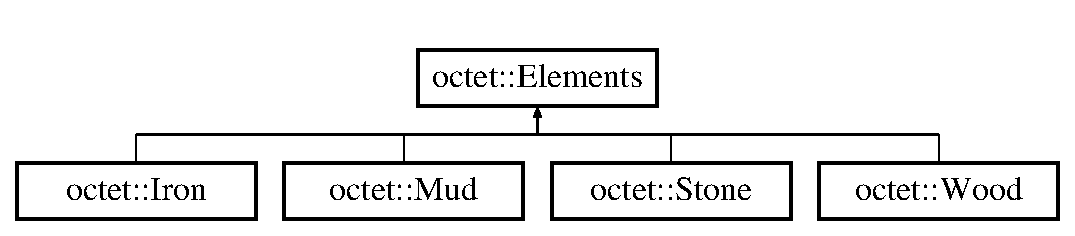
\includegraphics[height=2.000000cm]{structoctet_1_1_elements}
\end{center}
\end{figure}
\subsection*{Public Member Functions}
\begin{DoxyCompactItemize}
\item 
\hyperlink{structoctet_1_1_elements_a72500eca591953a90acb6d66b9b426d5}{Elements} (int \+\_\+id, string \+\_\+tag, int \+\_\+index, float \+\_\+health, int \+\_\+hit\+\_\+to\+\_\+extract, vec4 \+\_\+color)
\begin{DoxyCompactList}\small\item\em The constructor for the element struct. \end{DoxyCompactList}\item 
bool \hyperlink{structoctet_1_1_elements_a7175c9c96fb78c7ad933ca88f8b88f84}{Got\+\_\+\+Hit} (float damage)
\begin{DoxyCompactList}\small\item\em The ammont of damage the element has taken from the \hyperlink{structoctet_1_1_a_i}{A\+I} returns false if element has health $<$0. \end{DoxyCompactList}\end{DoxyCompactItemize}
\subsection*{Public Attributes}
\begin{DoxyCompactItemize}
\item 
int \hyperlink{structoctet_1_1_elements_ad7862925baea3ff467671233e86c6584}{id}
\begin{DoxyCompactList}\small\item\em The I\+D of the element ie mud, stone , wood, iron. \end{DoxyCompactList}\item 
string \hyperlink{structoctet_1_1_elements_ad7bb712671fd59dfce732441b15ed6e9}{tag}
\begin{DoxyCompactList}\small\item\em The tag of the element. \end{DoxyCompactList}\item 
float \hyperlink{structoctet_1_1_elements_af9cece89e171f07841b897dfb9be4eba}{health}
\begin{DoxyCompactList}\small\item\em The current health of the element. \end{DoxyCompactList}\item 
int \hyperlink{structoctet_1_1_elements_a33a93377f7814a339d0b4bc0d8200c02}{hit\+\_\+to\+\_\+extraxt}
\begin{DoxyCompactList}\small\item\em The number of hits needed to extract the element. \end{DoxyCompactList}\item 
vec4 \hyperlink{structoctet_1_1_elements_adf503621aeb69c7112453a430e39f76e}{color}
\begin{DoxyCompactList}\small\item\em the colour to be put out on the mesh \end{DoxyCompactList}\item 
int \hyperlink{structoctet_1_1_elements_a8d2c5872a3c685832f767505c85cf7e3}{index}
\begin{DoxyCompactList}\small\item\em The Index of this class in Game\+Object dynarry. \end{DoxyCompactList}\end{DoxyCompactItemize}


\subsection{Detailed Description}
The base struct for all the elements.\+Use this in the userpointer and call the derived class constructors to init this This is the object class for all the elements. 

\subsection{Constructor \& Destructor Documentation}
\hypertarget{structoctet_1_1_elements_a72500eca591953a90acb6d66b9b426d5}{\index{octet\+::\+Elements@{octet\+::\+Elements}!Elements@{Elements}}
\index{Elements@{Elements}!octet\+::\+Elements@{octet\+::\+Elements}}
\subsubsection[{Elements}]{\setlength{\rightskip}{0pt plus 5cm}octet\+::\+Elements\+::\+Elements (
\begin{DoxyParamCaption}
\item[{int}]{\+\_\+id, }
\item[{string}]{\+\_\+tag, }
\item[{int}]{\+\_\+index, }
\item[{float}]{\+\_\+health, }
\item[{int}]{\+\_\+hit\+\_\+to\+\_\+extract, }
\item[{vec4}]{\+\_\+color}
\end{DoxyParamCaption}
)\hspace{0.3cm}{\ttfamily [inline]}}}\label{structoctet_1_1_elements_a72500eca591953a90acb6d66b9b426d5}


The constructor for the element struct. 


\begin{DoxyParams}{Parameters}
{\em int} & \+\_\+id an int this is the id of the object to define if the object is mud,wood,stone,or iron ie I\+D\+\_\+\+Object \\
\hline
{\em string} & \+\_\+tag is the tag of the element \\
\hline
{\em int} & \+\_\+index the index in the gameobejct dynarray \\
\hline
{\em float} & \+\_\+health the health of the element \\
\hline
{\em int} & \+\_\+hit\+\_\+to\+\_\+extract the number of hits neede to extract \\
\hline
{\em vec4} & \+\_\+color the colour to be put out on the mesh \\
\hline
\end{DoxyParams}


\subsection{Member Function Documentation}
\hypertarget{structoctet_1_1_elements_a7175c9c96fb78c7ad933ca88f8b88f84}{\index{octet\+::\+Elements@{octet\+::\+Elements}!Got\+\_\+\+Hit@{Got\+\_\+\+Hit}}
\index{Got\+\_\+\+Hit@{Got\+\_\+\+Hit}!octet\+::\+Elements@{octet\+::\+Elements}}
\subsubsection[{Got\+\_\+\+Hit}]{\setlength{\rightskip}{0pt plus 5cm}bool octet\+::\+Elements\+::\+Got\+\_\+\+Hit (
\begin{DoxyParamCaption}
\item[{float}]{damage}
\end{DoxyParamCaption}
)\hspace{0.3cm}{\ttfamily [inline]}}}\label{structoctet_1_1_elements_a7175c9c96fb78c7ad933ca88f8b88f84}


The ammont of damage the element has taken from the \hyperlink{structoctet_1_1_a_i}{A\+I} returns false if element has health $<$0. 

\begin{DoxyReturn}{Returns}
a bool true if element has some health else false 
\end{DoxyReturn}


\subsection{Member Data Documentation}
\hypertarget{structoctet_1_1_elements_adf503621aeb69c7112453a430e39f76e}{\index{octet\+::\+Elements@{octet\+::\+Elements}!color@{color}}
\index{color@{color}!octet\+::\+Elements@{octet\+::\+Elements}}
\subsubsection[{color}]{\setlength{\rightskip}{0pt plus 5cm}vec4 octet\+::\+Elements\+::color}}\label{structoctet_1_1_elements_adf503621aeb69c7112453a430e39f76e}


the colour to be put out on the mesh 

\hypertarget{structoctet_1_1_elements_af9cece89e171f07841b897dfb9be4eba}{\index{octet\+::\+Elements@{octet\+::\+Elements}!health@{health}}
\index{health@{health}!octet\+::\+Elements@{octet\+::\+Elements}}
\subsubsection[{health}]{\setlength{\rightskip}{0pt plus 5cm}float octet\+::\+Elements\+::health}}\label{structoctet_1_1_elements_af9cece89e171f07841b897dfb9be4eba}


The current health of the element. 

\hypertarget{structoctet_1_1_elements_a33a93377f7814a339d0b4bc0d8200c02}{\index{octet\+::\+Elements@{octet\+::\+Elements}!hit\+\_\+to\+\_\+extraxt@{hit\+\_\+to\+\_\+extraxt}}
\index{hit\+\_\+to\+\_\+extraxt@{hit\+\_\+to\+\_\+extraxt}!octet\+::\+Elements@{octet\+::\+Elements}}
\subsubsection[{hit\+\_\+to\+\_\+extraxt}]{\setlength{\rightskip}{0pt plus 5cm}int octet\+::\+Elements\+::hit\+\_\+to\+\_\+extraxt}}\label{structoctet_1_1_elements_a33a93377f7814a339d0b4bc0d8200c02}


The number of hits needed to extract the element. 

\hypertarget{structoctet_1_1_elements_ad7862925baea3ff467671233e86c6584}{\index{octet\+::\+Elements@{octet\+::\+Elements}!id@{id}}
\index{id@{id}!octet\+::\+Elements@{octet\+::\+Elements}}
\subsubsection[{id}]{\setlength{\rightskip}{0pt plus 5cm}int octet\+::\+Elements\+::id}}\label{structoctet_1_1_elements_ad7862925baea3ff467671233e86c6584}


The I\+D of the element ie mud, stone , wood, iron. 

\hypertarget{structoctet_1_1_elements_a8d2c5872a3c685832f767505c85cf7e3}{\index{octet\+::\+Elements@{octet\+::\+Elements}!index@{index}}
\index{index@{index}!octet\+::\+Elements@{octet\+::\+Elements}}
\subsubsection[{index}]{\setlength{\rightskip}{0pt plus 5cm}int octet\+::\+Elements\+::index}}\label{structoctet_1_1_elements_a8d2c5872a3c685832f767505c85cf7e3}


The Index of this class in Game\+Object dynarry. 

\hypertarget{structoctet_1_1_elements_ad7bb712671fd59dfce732441b15ed6e9}{\index{octet\+::\+Elements@{octet\+::\+Elements}!tag@{tag}}
\index{tag@{tag}!octet\+::\+Elements@{octet\+::\+Elements}}
\subsubsection[{tag}]{\setlength{\rightskip}{0pt plus 5cm}string octet\+::\+Elements\+::tag}}\label{structoctet_1_1_elements_ad7bb712671fd59dfce732441b15ed6e9}


The tag of the element. 



The documentation for this struct was generated from the following file\+:\begin{DoxyCompactItemize}
\item 
\hyperlink{minecraft__wars_8h}{minecraft\+\_\+wars.\+h}\end{DoxyCompactItemize}

\hypertarget{structoctet_1_1_iron}{\section{octet\+:\+:Iron Struct Reference}
\label{structoctet_1_1_iron}\index{octet\+::\+Iron@{octet\+::\+Iron}}
}


{\ttfamily \#include $<$minecraft\+\_\+wars.\+h$>$}

Inheritance diagram for octet\+:\+:Iron\+:\begin{figure}[H]
\begin{center}
\leavevmode
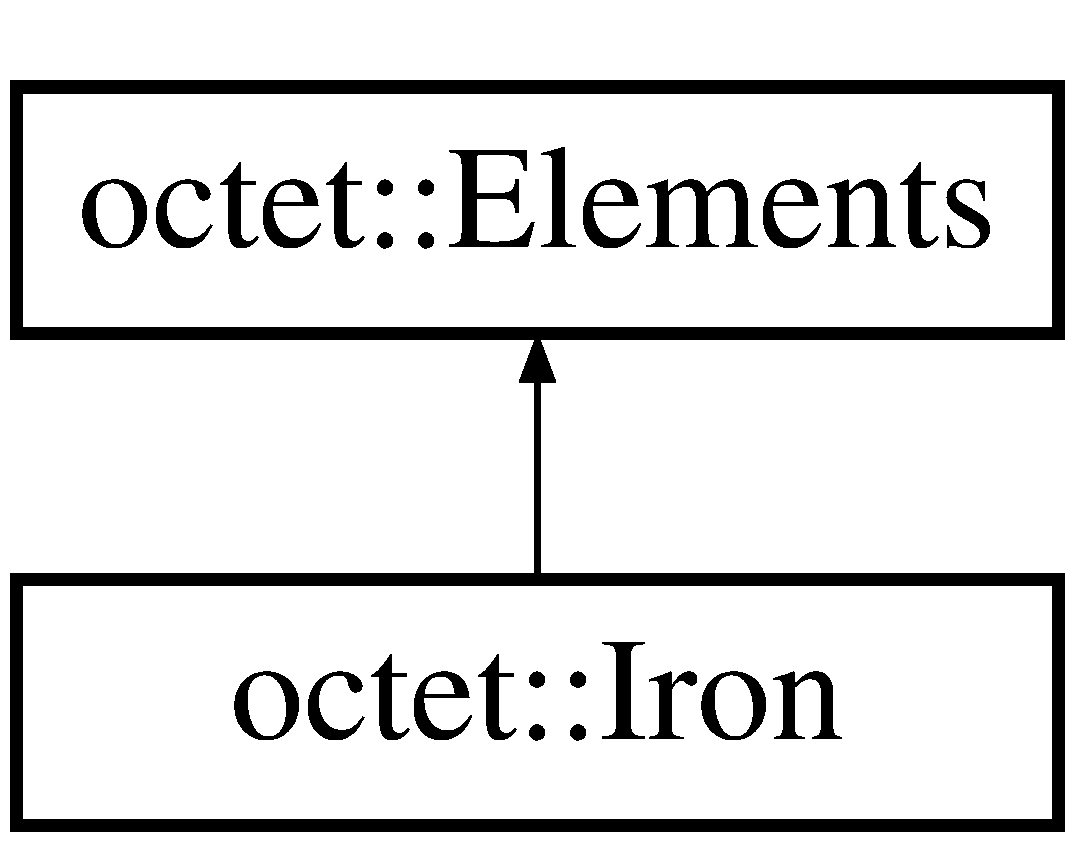
\includegraphics[height=2.000000cm]{structoctet_1_1_iron}
\end{center}
\end{figure}
\subsection*{Public Member Functions}
\begin{DoxyCompactItemize}
\item 
\hyperlink{structoctet_1_1_iron_a3979b06d9954e69ad635a05a10cf84af}{Iron} (int \hyperlink{structoctet_1_1_elements_a8d2c5872a3c685832f767505c85cf7e3}{index})
\end{DoxyCompactItemize}
\subsection*{Additional Inherited Members}


\subsection{Constructor \& Destructor Documentation}
\hypertarget{structoctet_1_1_iron_a3979b06d9954e69ad635a05a10cf84af}{\index{octet\+::\+Iron@{octet\+::\+Iron}!Iron@{Iron}}
\index{Iron@{Iron}!octet\+::\+Iron@{octet\+::\+Iron}}
\subsubsection[{Iron}]{\setlength{\rightskip}{0pt plus 5cm}octet\+::\+Iron\+::\+Iron (
\begin{DoxyParamCaption}
\item[{int}]{index}
\end{DoxyParamCaption}
)\hspace{0.3cm}{\ttfamily [inline]}}}\label{structoctet_1_1_iron_a3979b06d9954e69ad635a05a10cf84af}


The documentation for this struct was generated from the following file\+:\begin{DoxyCompactItemize}
\item 
\hyperlink{minecraft__wars_8h}{minecraft\+\_\+wars.\+h}\end{DoxyCompactItemize}

\hypertarget{classoctet_1_1minecraft__wars}{\section{octet\+:\+:minecraft\+\_\+wars Class Reference}
\label{classoctet_1_1minecraft__wars}\index{octet\+::minecraft\+\_\+wars@{octet\+::minecraft\+\_\+wars}}
}


this is the main class of this project.  




{\ttfamily \#include $<$minecraft\+\_\+wars.\+h$>$}

Inheritance diagram for octet\+:\+:minecraft\+\_\+wars\+:\begin{figure}[H]
\begin{center}
\leavevmode
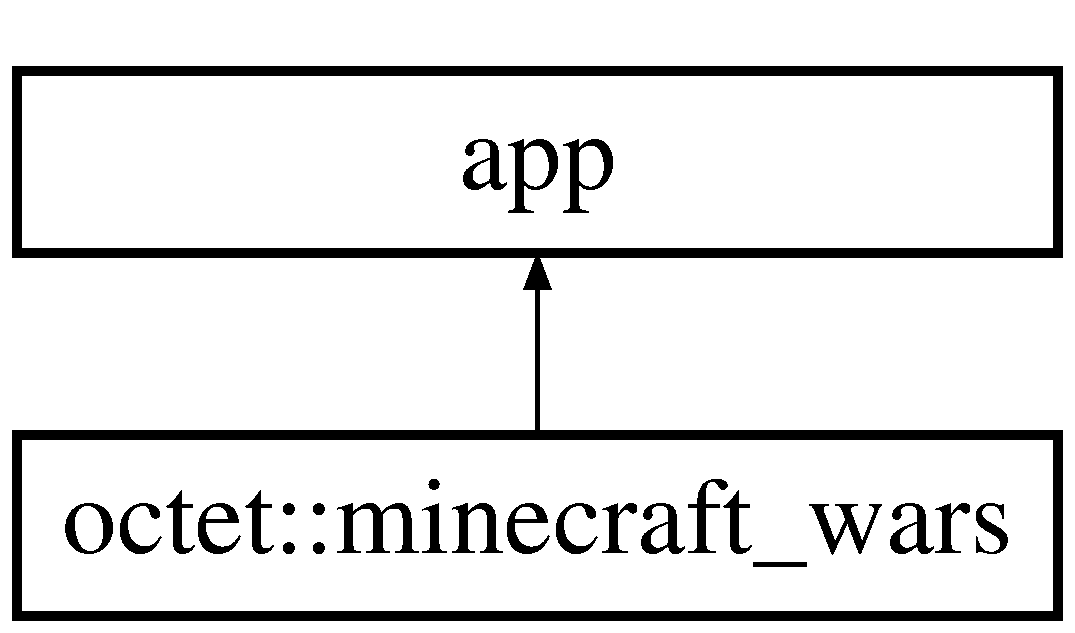
\includegraphics[height=2.000000cm]{classoctet_1_1minecraft__wars}
\end{center}
\end{figure}
\subsection*{Public Member Functions}
\begin{DoxyCompactItemize}
\item 
\hyperlink{classoctet_1_1minecraft__wars_acae462db6a97b0f3f2010a3d6fdda734}{minecraft\+\_\+wars} (int argc, char $\ast$$\ast$argv)
\begin{DoxyCompactList}\small\item\em this is called when we construct the class before everything is initialised. \end{DoxyCompactList}\item 
\hyperlink{classoctet_1_1minecraft__wars_af51fd5e1f5613ad1e2b78b9a1132a27d}{$\sim$minecraft\+\_\+wars} ()
\item 
void \hyperlink{classoctet_1_1minecraft__wars_a4d7e0650790969c0ecf286deab0c2b63}{app\+\_\+init} ()
\begin{DoxyCompactList}\small\item\em this is called once Open\+G\+L is initialized \end{DoxyCompactList}\item 
void \hyperlink{classoctet_1_1minecraft__wars_a483435b1af8285d343873eeecaaeca0a}{draw\+\_\+world} (int x, int y, int w, int h)
\begin{DoxyCompactList}\small\item\em this is called to draw the world \end{DoxyCompactList}\end{DoxyCompactItemize}
\subsection*{Private Types}
\begin{DoxyCompactItemize}
\item 
enum \hyperlink{classoctet_1_1minecraft__wars_ac30cfc7ec58748224e1109e398522462}{Num\+\_\+sound} \{ \hyperlink{classoctet_1_1minecraft__wars_ac30cfc7ec58748224e1109e398522462ad12e509a5562df299a02b60456736c9c}{Num\+\_\+shoot} = 0, 
\hyperlink{classoctet_1_1minecraft__wars_ac30cfc7ec58748224e1109e398522462a13f24fe7cd8f02bf8ddb88d86fb0636a}{Num\+\_\+place}, 
\hyperlink{classoctet_1_1minecraft__wars_ac30cfc7ec58748224e1109e398522462a5dafe8fadc6f2962ad5c79cbd479a029}{Num\+\_\+gather}, 
\hyperlink{classoctet_1_1minecraft__wars_ac30cfc7ec58748224e1109e398522462a6e8de0b5836c4b4d830394c609538558}{Num\+\_\+zombieattack}
 \}
\begin{DoxyCompactList}\small\item\em The enum for the sound. \end{DoxyCompactList}\item 
enum \hyperlink{classoctet_1_1minecraft__wars_a5d719db7b0232a40272505d0c4e56281}{Popup\+\_\+\+Msg} \{ \\*
\hyperlink{classoctet_1_1minecraft__wars_a5d719db7b0232a40272505d0c4e56281ab2b8322b755a8de1fc36fdddb83b15f1}{Msg\+\_\+\+None} = 0, 
\hyperlink{classoctet_1_1minecraft__wars_a5d719db7b0232a40272505d0c4e56281aa6dc49c36638c439e751ed67a7f6e448}{Msg\+\_\+\+Cant\+Place}, 
\hyperlink{classoctet_1_1minecraft__wars_a5d719db7b0232a40272505d0c4e56281a0cb5aa2311cc9e37a7513fbb16aa0736}{Msg\+\_\+\+Out\+Of\+Ammo}, 
\hyperlink{classoctet_1_1minecraft__wars_a5d719db7b0232a40272505d0c4e56281a54ac09e884d29d2a2a38d28b9cefe558}{Msg\+\_\+\+Zombies\+Active}, 
\\*
\hyperlink{classoctet_1_1minecraft__wars_a5d719db7b0232a40272505d0c4e56281a8019823abc3ab3b35d217ca7366f7240}{Msg\+\_\+\+Not\+Enough\+Elements}
 \}
\begin{DoxyCompactList}\small\item\em The enum for the popup msg. \end{DoxyCompactList}\end{DoxyCompactItemize}
\subsection*{Private Member Functions}
\begin{DoxyCompactItemize}
\item 
A\+Luint \hyperlink{classoctet_1_1minecraft__wars_ae988d46dbc1d01cd23bc6537f1ee0a48}{get\+\_\+sound\+\_\+source} (int s)
\begin{DoxyCompactList}\small\item\em returns the sound to play \end{DoxyCompactList}\item 
void \hyperlink{classoctet_1_1minecraft__wars_a73ae144486185995823024e3e5cd492e}{mapmaker} ()
\begin{DoxyCompactList}\small\item\em this is used to make the map. ie set all the elements in the map \end{DoxyCompactList}\item 
void \hyperlink{classoctet_1_1minecraft__wars_a8ede0f5f9aeab879cdf150c43ea67eff}{Add\+\_\+\+Rigidbody\+\_\+to\+\_\+\+Cam} ()
\begin{DoxyCompactList}\small\item\em Attach a rigid body to the camera so that we can interact with the physics world. \end{DoxyCompactList}\item 
void \hyperlink{classoctet_1_1minecraft__wars_a995d28ddd52f75acd16d8abe8f2f2f20}{Create\+\_\+base} ()
\begin{DoxyCompactList}\small\item\em create a rigid body base for the game \end{DoxyCompactList}\item 
vec3 \hyperlink{classoctet_1_1minecraft__wars_a3b33cb6cef05571ad2072adcecafd47c}{matrixmult} (mat4t objm, vec3 direction)
\begin{DoxyCompactList}\small\item\em returns the postion of the point according to the object and the direction \end{DoxyCompactList}\item 
void \hyperlink{classoctet_1_1minecraft__wars_a95f7058870a6892289fc8bac7c60f714}{Player\+\_\+cont} ()
\begin{DoxyCompactList}\small\item\em The player controls ie gathering placing shooting walking jumping rotationg camera.... \end{DoxyCompactList}\item 
void \hyperlink{classoctet_1_1minecraft__wars_aab0d43a5ef97e3cd0693dd7afc2d026d}{gatheringelement} ()
\begin{DoxyCompactList}\small\item\em Used to count down the frames since the last gathering key was pressed so that the player can gather again. \end{DoxyCompactList}\item 
void \hyperlink{classoctet_1_1minecraft__wars_aa92f3102de51e3a9da328f5bb0b1fca9}{placingelement} ()
\begin{DoxyCompactList}\small\item\em Used to count down the frames since the last placing key was pressed. after the timer elapses the object is placed. \end{DoxyCompactList}\item 
void \hyperlink{classoctet_1_1minecraft__wars_a012f43869f4e1812d2b3467e16aeb694}{shootreload} ()
\begin{DoxyCompactList}\small\item\em Used to count down the frames since the last shoot was fired. \end{DoxyCompactList}\item 
void \hyperlink{classoctet_1_1minecraft__wars_a1143a19dccab97d4227c2025a2c34b22}{waitforjump} ()
\begin{DoxyCompactList}\small\item\em Used to count down the frames since the last jump key was pressed so that the player can jump again. \end{DoxyCompactList}\item 
void \hyperlink{classoctet_1_1minecraft__wars_a72b700a60ce62322465331f8b1ae4f76}{activateenemies} ()
\begin{DoxyCompactList}\small\item\em This function is used to create enemies with random postion. This function is only called on the first night. \end{DoxyCompactList}\item 
void \hyperlink{classoctet_1_1minecraft__wars_a3afad7348f73707dc4bb39002d791856}{enemyconts} ()
\begin{DoxyCompactList}\small\item\em The \hyperlink{structoctet_1_1_a_i}{A\+I} controls ie run after the player and attack. \end{DoxyCompactList}\item 
void \hyperlink{classoctet_1_1minecraft__wars_a775fc0daacbea14fe01b1e72185e67c9}{killallenemies} ()
\begin{DoxyCompactList}\small\item\em This function is used to kill all the enemies when the night ends. \end{DoxyCompactList}\item 
void \hyperlink{classoctet_1_1minecraft__wars_aded48a159d7e20a3a3179d99bcd58435}{recycle\+\_\+enemies} (int \+\_\+index)
\begin{DoxyCompactList}\small\item\em This fucntion is used to reiniti the dead enemy and place him at a random loaction this function is only called in night time. \end{DoxyCompactList}\item 
void \hyperlink{classoctet_1_1minecraft__wars_afb34a43009cfc0baab3aa513a4dc66ed}{recycleallenemies} ()
\begin{DoxyCompactList}\small\item\em This function is called from the second night to reiniti all the dead enemy and place him at a random loaction this function is only called in night time. \end{DoxyCompactList}\item 
void \hyperlink{classoctet_1_1minecraft__wars_a7af21c40db01d09ba2af5e456149446c}{init\+\_\+shingingbox} ()
\begin{DoxyCompactList}\small\item\em This function is used to init the lighing shader. \end{DoxyCompactList}\item 
void \hyperlink{classoctet_1_1minecraft__wars_a605d1a677b8a449404efeb2e61d1183e}{init\+\_\+player\+\_\+var} ()
\begin{DoxyCompactList}\small\item\em This function is used to init the player vars ie gathering palcing shooting canjump canshoot...... \end{DoxyCompactList}\item 
void \hyperlink{classoctet_1_1minecraft__wars_a7db53f6134296b16d3919f1329fd5ca4}{clearpopup} ()
\begin{DoxyCompactList}\small\item\em This function is used clear the popup U\+I after the framecount elapse. \end{DoxyCompactList}\item 
void \hyperlink{classoctet_1_1minecraft__wars_ab20e3245b90dcbf9b63bef3189e844e8}{init\+U\+I} ()
\begin{DoxyCompactList}\small\item\em This function is used to init the U\+I variables ie overlay textmesh.... \end{DoxyCompactList}\item 
void \hyperlink{classoctet_1_1minecraft__wars_aea40090026e3facc7caf198b41211c7a}{update\+U\+I} (int vx, int vy)
\begin{DoxyCompactList}\small\item\em This function is used update the U\+I. \end{DoxyCompactList}\item 
void \hyperlink{classoctet_1_1minecraft__wars_ab84c69192d90263fb5ae0280b7f0d325}{Init\+Day\+Night\+Cycle} ()
\begin{DoxyCompactList}\small\item\em This function is used to init the day night cycle. \end{DoxyCompactList}\item 
void \hyperlink{classoctet_1_1minecraft__wars_af4b0e7ecdbaa960f7e4b39c05d2b84ad}{Day\+Night\+Cycle} ()
\begin{DoxyCompactList}\small\item\em This function is used to mantain the day night cycle. Ie the movement of the sun and the moon and the spawning and recycling of the enemies. \end{DoxyCompactList}\end{DoxyCompactItemize}
\subsection*{Private Attributes}
\begin{DoxyCompactItemize}
\item 
ref$<$ visual\+\_\+scene $>$ \hyperlink{classoctet_1_1minecraft__wars_ac96956a574d5aa5a30a84de7e226bd34}{app\+\_\+scene}
\begin{DoxyCompactList}\small\item\em scene for drawing box \end{DoxyCompactList}\item 
bt\+Default\+Collision\+Configuration \hyperlink{classoctet_1_1minecraft__wars_a0c7e9c9bea5aa8288253f9617d02967c}{config}
\begin{DoxyCompactList}\small\item\em setup for the world \end{DoxyCompactList}\item 
bt\+Collision\+Dispatcher $\ast$ \hyperlink{classoctet_1_1minecraft__wars_aeff7b8c9d268bc27c1dcf5ddac645cc9}{dispatcher}
\begin{DoxyCompactList}\small\item\em handler for collisions between objects \end{DoxyCompactList}\item 
bt\+Dbvt\+Broadphase $\ast$ \hyperlink{classoctet_1_1minecraft__wars_a3f2bdb1f69ade79860ca22618cef0040}{broadphase}
\begin{DoxyCompactList}\small\item\em handler for broadphase (rough) collision \end{DoxyCompactList}\item 
bt\+Sequential\+Impulse\+Constraint\+Solver $\ast$ \hyperlink{classoctet_1_1minecraft__wars_adbb4181c0f1c875551b55294cb6e3fca}{solver}
\begin{DoxyCompactList}\small\item\em handler to resolve collisions \end{DoxyCompactList}\item 
bt\+Discrete\+Dynamics\+World $\ast$ \hyperlink{classoctet_1_1minecraft__wars_ad609d762782c6f823aec20fc26dfae00}{world}
\begin{DoxyCompactList}\small\item\em physics world, contains rigid bodies \end{DoxyCompactList}\item 
\hyperlink{structoctet_1_1_player}{Player} \hyperlink{classoctet_1_1minecraft__wars_a645d3de2d70d3db06ca3762d75e5218c}{The\+\_\+\+Player}
\begin{DoxyCompactList}\small\item\em the player (which will be linked to the user pointer of the rigid bodies of the player) \end{DoxyCompactList}\item 
dynarray$<$ \hyperlink{classoctet_1_1_collision_objects}{Collision\+Objects} $\ast$ $>$ \hyperlink{classoctet_1_1minecraft__wars_ace75749e2bc41e51eafd0e44b0670b8b}{Game\+\_\+objects}
\begin{DoxyCompactList}\small\item\em the game objects this contains the rigidbodies gameobj class and the id for the object. \end{DoxyCompactList}\item 
dynarray$<$ scene\+\_\+node $\ast$ $>$ \hyperlink{classoctet_1_1minecraft__wars_a2ef2f751e20910c5fd0bdeca72a9a592}{nodes}
\begin{DoxyCompactList}\small\item\em the nodes for the game just used for the rendering \end{DoxyCompactList}\item 
dynarray$<$ \hyperlink{classoctet_1_1_collision_objects}{Collision\+Objects} $\ast$ $>$ \hyperlink{classoctet_1_1minecraft__wars_af16a3ace67e10fe889a385b8ab8405cb}{Enemies}
\begin{DoxyCompactList}\small\item\em the \hyperlink{classoctet_1_1_collision_objects}{Collision\+Objects} for the enemies, used to contr the enemies \end{DoxyCompactList}\item 
bool \hyperlink{classoctet_1_1minecraft__wars_ae02d056bcc40e7b09635ab2856d8d5d7}{gathering}
\begin{DoxyCompactList}\small\item\em this indicates that the player is gather so wait for some frames till the next time player can gather \end{DoxyCompactList}\item 
bool \hyperlink{classoctet_1_1minecraft__wars_ad801da09f504cde20563c2fe46e196e1}{placing}
\begin{DoxyCompactList}\small\item\em this indicates that the player is placing something \end{DoxyCompactList}\item 
bool \hyperlink{classoctet_1_1minecraft__wars_a33d14857ff44463f24ca76747c762745}{canshoot}
\begin{DoxyCompactList}\small\item\em true if player can shoot; if he has shot then make this false and true again after set frames \end{DoxyCompactList}\item 
float \hyperlink{classoctet_1_1minecraft__wars_a103c8c498e1a7a0bcddf22bb4ea4267f}{framecount\+\_\+gathering}
\begin{DoxyCompactList}\small\item\em multiplay this with 30$\ast$nu of sec to collect the item and then chk of frams \end{DoxyCompactList}\item 
float \hyperlink{classoctet_1_1minecraft__wars_a16ff1afbb738dec45fe41a8c90caf3d9}{tempframe\+\_\+gathering}
\begin{DoxyCompactList}\small\item\em set =0 when gathering chk with framecount to see if can gather or not \end{DoxyCompactList}\item 
float \hyperlink{classoctet_1_1minecraft__wars_a5cb24438a620f2ae64a95c3dcf58f0bb}{framecount\+\_\+shooting}
\item 
float \hyperlink{classoctet_1_1minecraft__wars_ac0f39aace1058f32df099906feed5f72}{tempframe\+\_\+shooting}
\begin{DoxyCompactList}\small\item\em set =0 when shooting chk with framecount to see if can gather or not \end{DoxyCompactList}\item 
float \hyperlink{classoctet_1_1minecraft__wars_aeb0766394c72986b610e8c7e513ff81b}{framecount\+\_\+placing}
\item 
float \hyperlink{classoctet_1_1minecraft__wars_a702c765ff3b72d26326f0c23dafee7b5}{tempframe\+\_\+placing}
\begin{DoxyCompactList}\small\item\em set =0 when placing chk with framecount to see if can gather or not \end{DoxyCompactList}\item 
bool \hyperlink{classoctet_1_1minecraft__wars_abf8f37ba4570f98b1361919b56460df2}{canjump}
\begin{DoxyCompactList}\small\item\em true if the player can jump false if he cant \end{DoxyCompactList}\item 
float \hyperlink{classoctet_1_1minecraft__wars_a3b1687fe91e29d83e0c854b7ff101104}{framecount\+\_\+jump}
\begin{DoxyCompactList}\small\item\em multiplay this with 30$\ast$nu of sec to jump and then chk of frams \end{DoxyCompactList}\item 
float \hyperlink{classoctet_1_1minecraft__wars_aa931e9fbabfd6f4e34be1d347c0f3243}{tempframecount\+\_\+jump}
\begin{DoxyCompactList}\small\item\em set =0 when jump chk with framecount to see if can jump or not \end{DoxyCompactList}\item 
float \hyperlink{classoctet_1_1minecraft__wars_aad3088aab37dfa4958679db1811faa5a}{tempframe\+\_\+place\+\_\+enemy}
\begin{DoxyCompactList}\small\item\em used as a seed to ramdomize the position of the enemy \end{DoxyCompactList}\item 
float \hyperlink{classoctet_1_1minecraft__wars_ac51eb660e901c04fe7d3b7803d32323e}{nu\+\_\+enemies}
\begin{DoxyCompactList}\small\item\em number of enemies to make \end{DoxyCompactList}\item 
bool \hyperlink{classoctet_1_1minecraft__wars_ae0d291f49dc8f23c1bab8d1bc53b2c5d}{activate\+\_\+enemies}
\begin{DoxyCompactList}\small\item\em activate the enemies in the night and deactivate in the morning \end{DoxyCompactList}\item 
\hyperlink{structoctet_1_1_elements}{Elements} $\ast$ \hyperlink{classoctet_1_1minecraft__wars_a2737ea29048537da921679cd2c0d1885}{element}
\begin{DoxyCompactList}\small\item\em the element we are gathering \end{DoxyCompactList}\item 
bt\+Collision\+Shape $\ast$ \hyperlink{classoctet_1_1minecraft__wars_a76be6b7555e4fed213a4846bde7d3ba0}{elementshape}
\begin{DoxyCompactList}\small\item\em the collision shape used to make elements \end{DoxyCompactList}\item 
bt\+Collision\+Shape $\ast$ \hyperlink{classoctet_1_1minecraft__wars_aa3d199d2f6084140c89c884bb079fb7b}{enemyshape}
\begin{DoxyCompactList}\small\item\em the collision shape used to make enemies \end{DoxyCompactList}\item 
param\+\_\+shader $\ast$ \hyperlink{classoctet_1_1minecraft__wars_a2e5ca51c2373b40b1613c9ad818f7a39}{b}
\begin{DoxyCompactList}\small\item\em the lighting shader \end{DoxyCompactList}\item 
ref$<$ param\+\_\+uniform $>$ \hyperlink{classoctet_1_1minecraft__wars_af42f249968d7364bf5ebaf34aa04e86c}{m\+\_\+amb}
\begin{DoxyCompactList}\small\item\em the material ambient paramerter for the lighting shader. \end{DoxyCompactList}\item 
ref$<$ param\+\_\+uniform $>$ \hyperlink{classoctet_1_1minecraft__wars_aca1e4733d35f84e6e7beb0922091071a}{l\+\_\+amb}
\begin{DoxyCompactList}\small\item\em the light ambient paramerter for the lighting shader. \end{DoxyCompactList}\item 
ref$<$ param\+\_\+uniform $>$ \hyperlink{classoctet_1_1minecraft__wars_a6e9f0bc04242d7dc02663e0d8a385865}{m\+\_\+dif}
\begin{DoxyCompactList}\small\item\em the material diffuse paramerter for the lighting shader. \end{DoxyCompactList}\item 
ref$<$ param\+\_\+uniform $>$ \hyperlink{classoctet_1_1minecraft__wars_ac4e627b56678402ff9581a24725d17c0}{l\+\_\+dif}
\begin{DoxyCompactList}\small\item\em the light diffuse paramerter for the lighting shader. \end{DoxyCompactList}\item 
ref$<$ param\+\_\+uniform $>$ \hyperlink{classoctet_1_1minecraft__wars_a80007ff61c9366fbb63a374b224da78e}{m\+\_\+spec}
\begin{DoxyCompactList}\small\item\em the material specular paramerter for the lighting shader. \end{DoxyCompactList}\item 
ref$<$ param\+\_\+uniform $>$ \hyperlink{classoctet_1_1minecraft__wars_a6ef89c983e9b97bb1569a6962cb5417f}{l\+\_\+spec}
\begin{DoxyCompactList}\small\item\em the light specular paramerter for the lighting shader. \end{DoxyCompactList}\item 
ref$<$ param\+\_\+uniform $>$ \hyperlink{classoctet_1_1minecraft__wars_ae1bffb6f992f549b9f5664b9c81e114b}{shnn}
\begin{DoxyCompactList}\small\item\em the shining paramerter for the lighting shader. \end{DoxyCompactList}\item 
ref$<$ param\+\_\+uniform $>$ \hyperlink{classoctet_1_1minecraft__wars_aec22f87413969e6f3f86775d38e82ab3}{lightpos}
\begin{DoxyCompactList}\small\item\em the light position paramerter for the lighting shader. \end{DoxyCompactList}\item 
ref$<$ material $>$ \hyperlink{classoctet_1_1minecraft__wars_a13bdb9153c1d5fd497f5c0b7503d28d3}{shiningbox}
\begin{DoxyCompactList}\small\item\em the material for the lighting shader. \end{DoxyCompactList}\item 
float \hyperlink{classoctet_1_1minecraft__wars_a787dde65a444e4e71eb3994ced4a1f46}{shnnval} = 32
\item 
vec3 \hyperlink{classoctet_1_1minecraft__wars_acfbc3cf4a5d70d3885b38c220c2151ad}{amb}
\begin{DoxyCompactList}\small\item\em parameter value for the lighting shader. \end{DoxyCompactList}\item 
vec3 \hyperlink{classoctet_1_1minecraft__wars_a6b8b4cc7893ab6f361694de9d26d6336}{lamb}
\begin{DoxyCompactList}\small\item\em parameter value for the lighting shader. \end{DoxyCompactList}\item 
vec3 \hyperlink{classoctet_1_1minecraft__wars_affef81405c5dad0bc10c409781719645}{diff}
\begin{DoxyCompactList}\small\item\em parameter value for the lighting shader. \end{DoxyCompactList}\item 
vec3 \hyperlink{classoctet_1_1minecraft__wars_a8031b4e5055a0ae1a9ffe67a2cf4d168}{ldiff}
\begin{DoxyCompactList}\small\item\em parameter value for the lighting shader. \end{DoxyCompactList}\item 
vec3 \hyperlink{classoctet_1_1minecraft__wars_ab87766352cd67053cc6321ee3b50f0bd}{spec}
\begin{DoxyCompactList}\small\item\em parameter value for the lighting shader. \end{DoxyCompactList}\item 
vec3 \hyperlink{classoctet_1_1minecraft__wars_ae6f1a1adea97bff38101b79064781cea}{lspec}
\begin{DoxyCompactList}\small\item\em parameter value for the lighting shader. \end{DoxyCompactList}\item 
vec3 \hyperlink{classoctet_1_1minecraft__wars_adefdca5fc9d714ac66a152067de88899}{light\+\_\+pos}
\begin{DoxyCompactList}\small\item\em parameter value for the lighting shader. \end{DoxyCompactList}\item 
ref$<$ material $>$ \hyperlink{classoctet_1_1minecraft__wars_a4a9ebbe5825e5da5c6357718194e3d7e}{enemy\+\_\+material}
\begin{DoxyCompactList}\small\item\em parameter value for the lighting shader. \end{DoxyCompactList}\item 
text\+\_\+overlay $\ast$ \hyperlink{classoctet_1_1minecraft__wars_a91905856a8de4b1c973a89790ff17815}{overlay}
\begin{DoxyCompactList}\small\item\em text overlay for the U\+I. \end{DoxyCompactList}\item 
mesh\+\_\+text $\ast$ \hyperlink{classoctet_1_1minecraft__wars_aef4ef24e39d99f8c85f89869deebfd71}{U\+I\+\_\+top}
\begin{DoxyCompactList}\small\item\em text mesh for the top U\+I. \end{DoxyCompactList}\item 
mesh\+\_\+text $\ast$ \hyperlink{classoctet_1_1minecraft__wars_a8de450040dd8662f5743104bc8f54c71}{U\+I\+\_\+bot}
\begin{DoxyCompactList}\small\item\em text mesh for the bottom U\+I. \end{DoxyCompactList}\item 
mesh\+\_\+text $\ast$ \hyperlink{classoctet_1_1minecraft__wars_a3afa44a220796b1132b02c6ceb405fb1}{U\+I\+\_\+popup}
\begin{DoxyCompactList}\small\item\em text mesh for the popup U\+I. \end{DoxyCompactList}\item 
mesh\+\_\+text $\ast$ \hyperlink{classoctet_1_1minecraft__wars_a42fe53052b940a1b7f758e56156bbc3c}{target}
\begin{DoxyCompactList}\small\item\em text mesh for the target U\+I. \end{DoxyCompactList}\item 
int \hyperlink{classoctet_1_1minecraft__wars_aff5e77fadc9292cc353969851ee6e5ac}{popupmsg}
\begin{DoxyCompactList}\small\item\em The msg number for the pop up U\+I. \end{DoxyCompactList}\item 
int \hyperlink{classoctet_1_1minecraft__wars_af4669b717235fe938e43d8a6073ec3a9}{tempframpopup}
\begin{DoxyCompactList}\small\item\em The frames lapsed since the popup U\+I was on. \end{DoxyCompactList}\item 
int \hyperlink{classoctet_1_1minecraft__wars_ac65c7178370f1749467b5572bada9b36}{framepopup}
\begin{DoxyCompactList}\small\item\em The number of frames the popup U\+I should show up. \end{DoxyCompactList}\item 
A\+Luint \hyperlink{classoctet_1_1minecraft__wars_a8a76b75425f33dfe9a3895d5c1557e82}{Sound\+\_\+shoot}
\begin{DoxyCompactList}\small\item\em The sound for the gun. \end{DoxyCompactList}\item 
A\+Luint \hyperlink{classoctet_1_1minecraft__wars_a49c6d9bfd8211e8627e609be0be42f77}{Sound\+\_\+place}
\begin{DoxyCompactList}\small\item\em The sound for placing element. \end{DoxyCompactList}\item 
A\+Luint \hyperlink{classoctet_1_1minecraft__wars_a074eafb7ecaee55ddd999c8a9c26bb62}{Sound\+\_\+gather}
\begin{DoxyCompactList}\small\item\em The sound for gathering element. \end{DoxyCompactList}\item 
A\+Luint \hyperlink{classoctet_1_1minecraft__wars_ab065d64bf9df1a96bfd62b964b0c249e}{Sound\+\_\+zombieattak}
\begin{DoxyCompactList}\small\item\em The sound for zombie attack. \end{DoxyCompactList}\item 
A\+Luint \hyperlink{classoctet_1_1minecraft__wars_a2ee223674fa2fbe1616629725a6d845e}{sources} \mbox{[}4\mbox{]}
\begin{DoxyCompactList}\small\item\em The source for the sounds. \end{DoxyCompactList}\item 
bool \hyperlink{classoctet_1_1minecraft__wars_ad53fa9489507ea201f30c4a929dd0f77}{isday}
\begin{DoxyCompactList}\small\item\em true is its day, false if night \end{DoxyCompactList}\item 
int \hyperlink{classoctet_1_1minecraft__wars_a40e43deac31fa350abac00c6bb6eab75}{nightnumber}
\begin{DoxyCompactList}\small\item\em the number of nights that have passed \end{DoxyCompactList}\item 
bool \hyperlink{classoctet_1_1minecraft__wars_a0244d8a261eaeb616479c64ad2c0aab5}{enemiesrecycled}
\begin{DoxyCompactList}\small\item\em true if the enemies have been placed in the game , false if not (only used a trigger) \end{DoxyCompactList}\item 
float \hyperlink{classoctet_1_1minecraft__wars_aff5df5d4844cc380f26eb21b28537987}{gamedaytime}
\begin{DoxyCompactList}\small\item\em The game day night time (0-\/360) \end{DoxyCompactList}\item 
scene\+\_\+node $\ast$ \hyperlink{classoctet_1_1minecraft__wars_ac658c13a9f41b84fb89156ca0cb4b9f1}{daynightnode}
\begin{DoxyCompactList}\small\item\em The scene node for the day night cycle objects (sun and moon) \end{DoxyCompactList}\end{DoxyCompactItemize}


\subsection{Detailed Description}
this is the main class of this project. 

\subsection{Member Enumeration Documentation}
\hypertarget{classoctet_1_1minecraft__wars_ac30cfc7ec58748224e1109e398522462}{\index{octet\+::minecraft\+\_\+wars@{octet\+::minecraft\+\_\+wars}!Num\+\_\+sound@{Num\+\_\+sound}}
\index{Num\+\_\+sound@{Num\+\_\+sound}!octet\+::minecraft\+\_\+wars@{octet\+::minecraft\+\_\+wars}}
\subsubsection[{Num\+\_\+sound}]{\setlength{\rightskip}{0pt plus 5cm}enum {\bf octet\+::minecraft\+\_\+wars\+::\+Num\+\_\+sound}\hspace{0.3cm}{\ttfamily [private]}}}\label{classoctet_1_1minecraft__wars_ac30cfc7ec58748224e1109e398522462}


The enum for the sound. 

\begin{Desc}
\item[Enumerator]\par
\begin{description}
\index{Num\+\_\+shoot@{Num\+\_\+shoot}!octet\+::minecraft\+\_\+wars@{octet\+::minecraft\+\_\+wars}}\index{octet\+::minecraft\+\_\+wars@{octet\+::minecraft\+\_\+wars}!Num\+\_\+shoot@{Num\+\_\+shoot}}\item[{\em 
\hypertarget{classoctet_1_1minecraft__wars_ac30cfc7ec58748224e1109e398522462ad12e509a5562df299a02b60456736c9c}{Num\+\_\+shoot}\label{classoctet_1_1minecraft__wars_ac30cfc7ec58748224e1109e398522462ad12e509a5562df299a02b60456736c9c}
}]\index{Num\+\_\+place@{Num\+\_\+place}!octet\+::minecraft\+\_\+wars@{octet\+::minecraft\+\_\+wars}}\index{octet\+::minecraft\+\_\+wars@{octet\+::minecraft\+\_\+wars}!Num\+\_\+place@{Num\+\_\+place}}\item[{\em 
\hypertarget{classoctet_1_1minecraft__wars_ac30cfc7ec58748224e1109e398522462a13f24fe7cd8f02bf8ddb88d86fb0636a}{Num\+\_\+place}\label{classoctet_1_1minecraft__wars_ac30cfc7ec58748224e1109e398522462a13f24fe7cd8f02bf8ddb88d86fb0636a}
}]\index{Num\+\_\+gather@{Num\+\_\+gather}!octet\+::minecraft\+\_\+wars@{octet\+::minecraft\+\_\+wars}}\index{octet\+::minecraft\+\_\+wars@{octet\+::minecraft\+\_\+wars}!Num\+\_\+gather@{Num\+\_\+gather}}\item[{\em 
\hypertarget{classoctet_1_1minecraft__wars_ac30cfc7ec58748224e1109e398522462a5dafe8fadc6f2962ad5c79cbd479a029}{Num\+\_\+gather}\label{classoctet_1_1minecraft__wars_ac30cfc7ec58748224e1109e398522462a5dafe8fadc6f2962ad5c79cbd479a029}
}]\index{Num\+\_\+zombieattack@{Num\+\_\+zombieattack}!octet\+::minecraft\+\_\+wars@{octet\+::minecraft\+\_\+wars}}\index{octet\+::minecraft\+\_\+wars@{octet\+::minecraft\+\_\+wars}!Num\+\_\+zombieattack@{Num\+\_\+zombieattack}}\item[{\em 
\hypertarget{classoctet_1_1minecraft__wars_ac30cfc7ec58748224e1109e398522462a6e8de0b5836c4b4d830394c609538558}{Num\+\_\+zombieattack}\label{classoctet_1_1minecraft__wars_ac30cfc7ec58748224e1109e398522462a6e8de0b5836c4b4d830394c609538558}
}]\end{description}
\end{Desc}
\hypertarget{classoctet_1_1minecraft__wars_a5d719db7b0232a40272505d0c4e56281}{\index{octet\+::minecraft\+\_\+wars@{octet\+::minecraft\+\_\+wars}!Popup\+\_\+\+Msg@{Popup\+\_\+\+Msg}}
\index{Popup\+\_\+\+Msg@{Popup\+\_\+\+Msg}!octet\+::minecraft\+\_\+wars@{octet\+::minecraft\+\_\+wars}}
\subsubsection[{Popup\+\_\+\+Msg}]{\setlength{\rightskip}{0pt plus 5cm}enum {\bf octet\+::minecraft\+\_\+wars\+::\+Popup\+\_\+\+Msg}\hspace{0.3cm}{\ttfamily [private]}}}\label{classoctet_1_1minecraft__wars_a5d719db7b0232a40272505d0c4e56281}


The enum for the popup msg. 

\begin{Desc}
\item[Enumerator]\par
\begin{description}
\index{Msg\+\_\+\+None@{Msg\+\_\+\+None}!octet\+::minecraft\+\_\+wars@{octet\+::minecraft\+\_\+wars}}\index{octet\+::minecraft\+\_\+wars@{octet\+::minecraft\+\_\+wars}!Msg\+\_\+\+None@{Msg\+\_\+\+None}}\item[{\em 
\hypertarget{classoctet_1_1minecraft__wars_a5d719db7b0232a40272505d0c4e56281ab2b8322b755a8de1fc36fdddb83b15f1}{Msg\+\_\+\+None}\label{classoctet_1_1minecraft__wars_a5d719db7b0232a40272505d0c4e56281ab2b8322b755a8de1fc36fdddb83b15f1}
}]\index{Msg\+\_\+\+Cant\+Place@{Msg\+\_\+\+Cant\+Place}!octet\+::minecraft\+\_\+wars@{octet\+::minecraft\+\_\+wars}}\index{octet\+::minecraft\+\_\+wars@{octet\+::minecraft\+\_\+wars}!Msg\+\_\+\+Cant\+Place@{Msg\+\_\+\+Cant\+Place}}\item[{\em 
\hypertarget{classoctet_1_1minecraft__wars_a5d719db7b0232a40272505d0c4e56281aa6dc49c36638c439e751ed67a7f6e448}{Msg\+\_\+\+Cant\+Place}\label{classoctet_1_1minecraft__wars_a5d719db7b0232a40272505d0c4e56281aa6dc49c36638c439e751ed67a7f6e448}
}]\index{Msg\+\_\+\+Out\+Of\+Ammo@{Msg\+\_\+\+Out\+Of\+Ammo}!octet\+::minecraft\+\_\+wars@{octet\+::minecraft\+\_\+wars}}\index{octet\+::minecraft\+\_\+wars@{octet\+::minecraft\+\_\+wars}!Msg\+\_\+\+Out\+Of\+Ammo@{Msg\+\_\+\+Out\+Of\+Ammo}}\item[{\em 
\hypertarget{classoctet_1_1minecraft__wars_a5d719db7b0232a40272505d0c4e56281a0cb5aa2311cc9e37a7513fbb16aa0736}{Msg\+\_\+\+Out\+Of\+Ammo}\label{classoctet_1_1minecraft__wars_a5d719db7b0232a40272505d0c4e56281a0cb5aa2311cc9e37a7513fbb16aa0736}
}]\index{Msg\+\_\+\+Zombies\+Active@{Msg\+\_\+\+Zombies\+Active}!octet\+::minecraft\+\_\+wars@{octet\+::minecraft\+\_\+wars}}\index{octet\+::minecraft\+\_\+wars@{octet\+::minecraft\+\_\+wars}!Msg\+\_\+\+Zombies\+Active@{Msg\+\_\+\+Zombies\+Active}}\item[{\em 
\hypertarget{classoctet_1_1minecraft__wars_a5d719db7b0232a40272505d0c4e56281a54ac09e884d29d2a2a38d28b9cefe558}{Msg\+\_\+\+Zombies\+Active}\label{classoctet_1_1minecraft__wars_a5d719db7b0232a40272505d0c4e56281a54ac09e884d29d2a2a38d28b9cefe558}
}]\index{Msg\+\_\+\+Not\+Enough\+Elements@{Msg\+\_\+\+Not\+Enough\+Elements}!octet\+::minecraft\+\_\+wars@{octet\+::minecraft\+\_\+wars}}\index{octet\+::minecraft\+\_\+wars@{octet\+::minecraft\+\_\+wars}!Msg\+\_\+\+Not\+Enough\+Elements@{Msg\+\_\+\+Not\+Enough\+Elements}}\item[{\em 
\hypertarget{classoctet_1_1minecraft__wars_a5d719db7b0232a40272505d0c4e56281a8019823abc3ab3b35d217ca7366f7240}{Msg\+\_\+\+Not\+Enough\+Elements}\label{classoctet_1_1minecraft__wars_a5d719db7b0232a40272505d0c4e56281a8019823abc3ab3b35d217ca7366f7240}
}]\end{description}
\end{Desc}


\subsection{Constructor \& Destructor Documentation}
\hypertarget{classoctet_1_1minecraft__wars_acae462db6a97b0f3f2010a3d6fdda734}{\index{octet\+::minecraft\+\_\+wars@{octet\+::minecraft\+\_\+wars}!minecraft\+\_\+wars@{minecraft\+\_\+wars}}
\index{minecraft\+\_\+wars@{minecraft\+\_\+wars}!octet\+::minecraft\+\_\+wars@{octet\+::minecraft\+\_\+wars}}
\subsubsection[{minecraft\+\_\+wars}]{\setlength{\rightskip}{0pt plus 5cm}octet\+::minecraft\+\_\+wars\+::minecraft\+\_\+wars (
\begin{DoxyParamCaption}
\item[{int}]{argc, }
\item[{char $\ast$$\ast$}]{argv}
\end{DoxyParamCaption}
)\hspace{0.3cm}{\ttfamily [inline]}}}\label{classoctet_1_1minecraft__wars_acae462db6a97b0f3f2010a3d6fdda734}


this is called when we construct the class before everything is initialised. 

\hypertarget{classoctet_1_1minecraft__wars_af51fd5e1f5613ad1e2b78b9a1132a27d}{\index{octet\+::minecraft\+\_\+wars@{octet\+::minecraft\+\_\+wars}!````~minecraft\+\_\+wars@{$\sim$minecraft\+\_\+wars}}
\index{````~minecraft\+\_\+wars@{$\sim$minecraft\+\_\+wars}!octet\+::minecraft\+\_\+wars@{octet\+::minecraft\+\_\+wars}}
\subsubsection[{$\sim$minecraft\+\_\+wars}]{\setlength{\rightskip}{0pt plus 5cm}octet\+::minecraft\+\_\+wars\+::$\sim$minecraft\+\_\+wars (
\begin{DoxyParamCaption}
{}
\end{DoxyParamCaption}
)\hspace{0.3cm}{\ttfamily [inline]}}}\label{classoctet_1_1minecraft__wars_af51fd5e1f5613ad1e2b78b9a1132a27d}


\subsection{Member Function Documentation}
\hypertarget{classoctet_1_1minecraft__wars_a72b700a60ce62322465331f8b1ae4f76}{\index{octet\+::minecraft\+\_\+wars@{octet\+::minecraft\+\_\+wars}!activateenemies@{activateenemies}}
\index{activateenemies@{activateenemies}!octet\+::minecraft\+\_\+wars@{octet\+::minecraft\+\_\+wars}}
\subsubsection[{activateenemies}]{\setlength{\rightskip}{0pt plus 5cm}void octet\+::minecraft\+\_\+wars\+::activateenemies (
\begin{DoxyParamCaption}
{}
\end{DoxyParamCaption}
)\hspace{0.3cm}{\ttfamily [inline]}, {\ttfamily [private]}}}\label{classoctet_1_1minecraft__wars_a72b700a60ce62322465331f8b1ae4f76}


This function is used to create enemies with random postion. This function is only called on the first night. 

\hypertarget{classoctet_1_1minecraft__wars_a8ede0f5f9aeab879cdf150c43ea67eff}{\index{octet\+::minecraft\+\_\+wars@{octet\+::minecraft\+\_\+wars}!Add\+\_\+\+Rigidbody\+\_\+to\+\_\+\+Cam@{Add\+\_\+\+Rigidbody\+\_\+to\+\_\+\+Cam}}
\index{Add\+\_\+\+Rigidbody\+\_\+to\+\_\+\+Cam@{Add\+\_\+\+Rigidbody\+\_\+to\+\_\+\+Cam}!octet\+::minecraft\+\_\+wars@{octet\+::minecraft\+\_\+wars}}
\subsubsection[{Add\+\_\+\+Rigidbody\+\_\+to\+\_\+\+Cam}]{\setlength{\rightskip}{0pt plus 5cm}void octet\+::minecraft\+\_\+wars\+::\+Add\+\_\+\+Rigidbody\+\_\+to\+\_\+\+Cam (
\begin{DoxyParamCaption}
{}
\end{DoxyParamCaption}
)\hspace{0.3cm}{\ttfamily [inline]}, {\ttfamily [private]}}}\label{classoctet_1_1minecraft__wars_a8ede0f5f9aeab879cdf150c43ea67eff}


Attach a rigid body to the camera so that we can interact with the physics world. 

\hypertarget{classoctet_1_1minecraft__wars_a4d7e0650790969c0ecf286deab0c2b63}{\index{octet\+::minecraft\+\_\+wars@{octet\+::minecraft\+\_\+wars}!app\+\_\+init@{app\+\_\+init}}
\index{app\+\_\+init@{app\+\_\+init}!octet\+::minecraft\+\_\+wars@{octet\+::minecraft\+\_\+wars}}
\subsubsection[{app\+\_\+init}]{\setlength{\rightskip}{0pt plus 5cm}void octet\+::minecraft\+\_\+wars\+::app\+\_\+init (
\begin{DoxyParamCaption}
{}
\end{DoxyParamCaption}
)\hspace{0.3cm}{\ttfamily [inline]}}}\label{classoctet_1_1minecraft__wars_a4d7e0650790969c0ecf286deab0c2b63}


this is called once Open\+G\+L is initialized 

\hypertarget{classoctet_1_1minecraft__wars_a7db53f6134296b16d3919f1329fd5ca4}{\index{octet\+::minecraft\+\_\+wars@{octet\+::minecraft\+\_\+wars}!clearpopup@{clearpopup}}
\index{clearpopup@{clearpopup}!octet\+::minecraft\+\_\+wars@{octet\+::minecraft\+\_\+wars}}
\subsubsection[{clearpopup}]{\setlength{\rightskip}{0pt plus 5cm}void octet\+::minecraft\+\_\+wars\+::clearpopup (
\begin{DoxyParamCaption}
{}
\end{DoxyParamCaption}
)\hspace{0.3cm}{\ttfamily [inline]}, {\ttfamily [private]}}}\label{classoctet_1_1minecraft__wars_a7db53f6134296b16d3919f1329fd5ca4}


This function is used clear the popup U\+I after the framecount elapse. 

\hypertarget{classoctet_1_1minecraft__wars_a995d28ddd52f75acd16d8abe8f2f2f20}{\index{octet\+::minecraft\+\_\+wars@{octet\+::minecraft\+\_\+wars}!Create\+\_\+base@{Create\+\_\+base}}
\index{Create\+\_\+base@{Create\+\_\+base}!octet\+::minecraft\+\_\+wars@{octet\+::minecraft\+\_\+wars}}
\subsubsection[{Create\+\_\+base}]{\setlength{\rightskip}{0pt plus 5cm}void octet\+::minecraft\+\_\+wars\+::\+Create\+\_\+base (
\begin{DoxyParamCaption}
{}
\end{DoxyParamCaption}
)\hspace{0.3cm}{\ttfamily [inline]}, {\ttfamily [private]}}}\label{classoctet_1_1minecraft__wars_a995d28ddd52f75acd16d8abe8f2f2f20}


create a rigid body base for the game 

\hypertarget{classoctet_1_1minecraft__wars_af4b0e7ecdbaa960f7e4b39c05d2b84ad}{\index{octet\+::minecraft\+\_\+wars@{octet\+::minecraft\+\_\+wars}!Day\+Night\+Cycle@{Day\+Night\+Cycle}}
\index{Day\+Night\+Cycle@{Day\+Night\+Cycle}!octet\+::minecraft\+\_\+wars@{octet\+::minecraft\+\_\+wars}}
\subsubsection[{Day\+Night\+Cycle}]{\setlength{\rightskip}{0pt plus 5cm}void octet\+::minecraft\+\_\+wars\+::\+Day\+Night\+Cycle (
\begin{DoxyParamCaption}
{}
\end{DoxyParamCaption}
)\hspace{0.3cm}{\ttfamily [inline]}, {\ttfamily [private]}}}\label{classoctet_1_1minecraft__wars_af4b0e7ecdbaa960f7e4b39c05d2b84ad}


This function is used to mantain the day night cycle. Ie the movement of the sun and the moon and the spawning and recycling of the enemies. 

\hypertarget{classoctet_1_1minecraft__wars_a483435b1af8285d343873eeecaaeca0a}{\index{octet\+::minecraft\+\_\+wars@{octet\+::minecraft\+\_\+wars}!draw\+\_\+world@{draw\+\_\+world}}
\index{draw\+\_\+world@{draw\+\_\+world}!octet\+::minecraft\+\_\+wars@{octet\+::minecraft\+\_\+wars}}
\subsubsection[{draw\+\_\+world}]{\setlength{\rightskip}{0pt plus 5cm}void octet\+::minecraft\+\_\+wars\+::draw\+\_\+world (
\begin{DoxyParamCaption}
\item[{int}]{x, }
\item[{int}]{y, }
\item[{int}]{w, }
\item[{int}]{h}
\end{DoxyParamCaption}
)\hspace{0.3cm}{\ttfamily [inline]}}}\label{classoctet_1_1minecraft__wars_a483435b1af8285d343873eeecaaeca0a}


this is called to draw the world 

\hypertarget{classoctet_1_1minecraft__wars_a3afad7348f73707dc4bb39002d791856}{\index{octet\+::minecraft\+\_\+wars@{octet\+::minecraft\+\_\+wars}!enemyconts@{enemyconts}}
\index{enemyconts@{enemyconts}!octet\+::minecraft\+\_\+wars@{octet\+::minecraft\+\_\+wars}}
\subsubsection[{enemyconts}]{\setlength{\rightskip}{0pt plus 5cm}void octet\+::minecraft\+\_\+wars\+::enemyconts (
\begin{DoxyParamCaption}
{}
\end{DoxyParamCaption}
)\hspace{0.3cm}{\ttfamily [inline]}, {\ttfamily [private]}}}\label{classoctet_1_1minecraft__wars_a3afad7348f73707dc4bb39002d791856}


The \hyperlink{structoctet_1_1_a_i}{A\+I} controls ie run after the player and attack. 

\hypertarget{classoctet_1_1minecraft__wars_aab0d43a5ef97e3cd0693dd7afc2d026d}{\index{octet\+::minecraft\+\_\+wars@{octet\+::minecraft\+\_\+wars}!gatheringelement@{gatheringelement}}
\index{gatheringelement@{gatheringelement}!octet\+::minecraft\+\_\+wars@{octet\+::minecraft\+\_\+wars}}
\subsubsection[{gatheringelement}]{\setlength{\rightskip}{0pt plus 5cm}void octet\+::minecraft\+\_\+wars\+::gatheringelement (
\begin{DoxyParamCaption}
{}
\end{DoxyParamCaption}
)\hspace{0.3cm}{\ttfamily [inline]}, {\ttfamily [private]}}}\label{classoctet_1_1minecraft__wars_aab0d43a5ef97e3cd0693dd7afc2d026d}


Used to count down the frames since the last gathering key was pressed so that the player can gather again. 

\hypertarget{classoctet_1_1minecraft__wars_ae988d46dbc1d01cd23bc6537f1ee0a48}{\index{octet\+::minecraft\+\_\+wars@{octet\+::minecraft\+\_\+wars}!get\+\_\+sound\+\_\+source@{get\+\_\+sound\+\_\+source}}
\index{get\+\_\+sound\+\_\+source@{get\+\_\+sound\+\_\+source}!octet\+::minecraft\+\_\+wars@{octet\+::minecraft\+\_\+wars}}
\subsubsection[{get\+\_\+sound\+\_\+source}]{\setlength{\rightskip}{0pt plus 5cm}A\+Luint octet\+::minecraft\+\_\+wars\+::get\+\_\+sound\+\_\+source (
\begin{DoxyParamCaption}
\item[{int}]{s}
\end{DoxyParamCaption}
)\hspace{0.3cm}{\ttfamily [inline]}, {\ttfamily [private]}}}\label{classoctet_1_1minecraft__wars_ae988d46dbc1d01cd23bc6537f1ee0a48}


returns the sound to play 

\begin{DoxyReturn}{Returns}
a A\+Luint the sound to play 
\end{DoxyReturn}
\hypertarget{classoctet_1_1minecraft__wars_a605d1a677b8a449404efeb2e61d1183e}{\index{octet\+::minecraft\+\_\+wars@{octet\+::minecraft\+\_\+wars}!init\+\_\+player\+\_\+var@{init\+\_\+player\+\_\+var}}
\index{init\+\_\+player\+\_\+var@{init\+\_\+player\+\_\+var}!octet\+::minecraft\+\_\+wars@{octet\+::minecraft\+\_\+wars}}
\subsubsection[{init\+\_\+player\+\_\+var}]{\setlength{\rightskip}{0pt plus 5cm}void octet\+::minecraft\+\_\+wars\+::init\+\_\+player\+\_\+var (
\begin{DoxyParamCaption}
{}
\end{DoxyParamCaption}
)\hspace{0.3cm}{\ttfamily [inline]}, {\ttfamily [private]}}}\label{classoctet_1_1minecraft__wars_a605d1a677b8a449404efeb2e61d1183e}


This function is used to init the player vars ie gathering palcing shooting canjump canshoot...... 

\hypertarget{classoctet_1_1minecraft__wars_a7af21c40db01d09ba2af5e456149446c}{\index{octet\+::minecraft\+\_\+wars@{octet\+::minecraft\+\_\+wars}!init\+\_\+shingingbox@{init\+\_\+shingingbox}}
\index{init\+\_\+shingingbox@{init\+\_\+shingingbox}!octet\+::minecraft\+\_\+wars@{octet\+::minecraft\+\_\+wars}}
\subsubsection[{init\+\_\+shingingbox}]{\setlength{\rightskip}{0pt plus 5cm}void octet\+::minecraft\+\_\+wars\+::init\+\_\+shingingbox (
\begin{DoxyParamCaption}
{}
\end{DoxyParamCaption}
)\hspace{0.3cm}{\ttfamily [inline]}, {\ttfamily [private]}}}\label{classoctet_1_1minecraft__wars_a7af21c40db01d09ba2af5e456149446c}


This function is used to init the lighing shader. 

\hypertarget{classoctet_1_1minecraft__wars_ab84c69192d90263fb5ae0280b7f0d325}{\index{octet\+::minecraft\+\_\+wars@{octet\+::minecraft\+\_\+wars}!Init\+Day\+Night\+Cycle@{Init\+Day\+Night\+Cycle}}
\index{Init\+Day\+Night\+Cycle@{Init\+Day\+Night\+Cycle}!octet\+::minecraft\+\_\+wars@{octet\+::minecraft\+\_\+wars}}
\subsubsection[{Init\+Day\+Night\+Cycle}]{\setlength{\rightskip}{0pt plus 5cm}void octet\+::minecraft\+\_\+wars\+::\+Init\+Day\+Night\+Cycle (
\begin{DoxyParamCaption}
{}
\end{DoxyParamCaption}
)\hspace{0.3cm}{\ttfamily [inline]}, {\ttfamily [private]}}}\label{classoctet_1_1minecraft__wars_ab84c69192d90263fb5ae0280b7f0d325}


This function is used to init the day night cycle. 

\hypertarget{classoctet_1_1minecraft__wars_ab20e3245b90dcbf9b63bef3189e844e8}{\index{octet\+::minecraft\+\_\+wars@{octet\+::minecraft\+\_\+wars}!init\+U\+I@{init\+U\+I}}
\index{init\+U\+I@{init\+U\+I}!octet\+::minecraft\+\_\+wars@{octet\+::minecraft\+\_\+wars}}
\subsubsection[{init\+U\+I}]{\setlength{\rightskip}{0pt plus 5cm}void octet\+::minecraft\+\_\+wars\+::init\+U\+I (
\begin{DoxyParamCaption}
{}
\end{DoxyParamCaption}
)\hspace{0.3cm}{\ttfamily [inline]}, {\ttfamily [private]}}}\label{classoctet_1_1minecraft__wars_ab20e3245b90dcbf9b63bef3189e844e8}


This function is used to init the U\+I variables ie overlay textmesh.... 

\hypertarget{classoctet_1_1minecraft__wars_a775fc0daacbea14fe01b1e72185e67c9}{\index{octet\+::minecraft\+\_\+wars@{octet\+::minecraft\+\_\+wars}!killallenemies@{killallenemies}}
\index{killallenemies@{killallenemies}!octet\+::minecraft\+\_\+wars@{octet\+::minecraft\+\_\+wars}}
\subsubsection[{killallenemies}]{\setlength{\rightskip}{0pt plus 5cm}void octet\+::minecraft\+\_\+wars\+::killallenemies (
\begin{DoxyParamCaption}
{}
\end{DoxyParamCaption}
)\hspace{0.3cm}{\ttfamily [inline]}, {\ttfamily [private]}}}\label{classoctet_1_1minecraft__wars_a775fc0daacbea14fe01b1e72185e67c9}


This function is used to kill all the enemies when the night ends. 

\hypertarget{classoctet_1_1minecraft__wars_a73ae144486185995823024e3e5cd492e}{\index{octet\+::minecraft\+\_\+wars@{octet\+::minecraft\+\_\+wars}!mapmaker@{mapmaker}}
\index{mapmaker@{mapmaker}!octet\+::minecraft\+\_\+wars@{octet\+::minecraft\+\_\+wars}}
\subsubsection[{mapmaker}]{\setlength{\rightskip}{0pt plus 5cm}void octet\+::minecraft\+\_\+wars\+::mapmaker (
\begin{DoxyParamCaption}
{}
\end{DoxyParamCaption}
)\hspace{0.3cm}{\ttfamily [inline]}, {\ttfamily [private]}}}\label{classoctet_1_1minecraft__wars_a73ae144486185995823024e3e5cd492e}


this is used to make the map. ie set all the elements in the map 

\hypertarget{classoctet_1_1minecraft__wars_a3b33cb6cef05571ad2072adcecafd47c}{\index{octet\+::minecraft\+\_\+wars@{octet\+::minecraft\+\_\+wars}!matrixmult@{matrixmult}}
\index{matrixmult@{matrixmult}!octet\+::minecraft\+\_\+wars@{octet\+::minecraft\+\_\+wars}}
\subsubsection[{matrixmult}]{\setlength{\rightskip}{0pt plus 5cm}vec3 octet\+::minecraft\+\_\+wars\+::matrixmult (
\begin{DoxyParamCaption}
\item[{mat4t}]{objm, }
\item[{vec3}]{direction}
\end{DoxyParamCaption}
)\hspace{0.3cm}{\ttfamily [inline]}, {\ttfamily [private]}}}\label{classoctet_1_1minecraft__wars_a3b33cb6cef05571ad2072adcecafd47c}


returns the postion of the point according to the object and the direction 


\begin{DoxyParams}{Parameters}
{\em mat4t} & objm The parent matrix of the object \\
\hline
{\em vec3} & direction The direction we need to find ie front back left right \\
\hline
\end{DoxyParams}
\begin{DoxyReturn}{Returns}
a vec3 the postion of the point according to the object and the direction 
\end{DoxyReturn}
\hypertarget{classoctet_1_1minecraft__wars_aa92f3102de51e3a9da328f5bb0b1fca9}{\index{octet\+::minecraft\+\_\+wars@{octet\+::minecraft\+\_\+wars}!placingelement@{placingelement}}
\index{placingelement@{placingelement}!octet\+::minecraft\+\_\+wars@{octet\+::minecraft\+\_\+wars}}
\subsubsection[{placingelement}]{\setlength{\rightskip}{0pt plus 5cm}void octet\+::minecraft\+\_\+wars\+::placingelement (
\begin{DoxyParamCaption}
{}
\end{DoxyParamCaption}
)\hspace{0.3cm}{\ttfamily [inline]}, {\ttfamily [private]}}}\label{classoctet_1_1minecraft__wars_aa92f3102de51e3a9da328f5bb0b1fca9}


Used to count down the frames since the last placing key was pressed. after the timer elapses the object is placed. 

\hypertarget{classoctet_1_1minecraft__wars_a95f7058870a6892289fc8bac7c60f714}{\index{octet\+::minecraft\+\_\+wars@{octet\+::minecraft\+\_\+wars}!Player\+\_\+cont@{Player\+\_\+cont}}
\index{Player\+\_\+cont@{Player\+\_\+cont}!octet\+::minecraft\+\_\+wars@{octet\+::minecraft\+\_\+wars}}
\subsubsection[{Player\+\_\+cont}]{\setlength{\rightskip}{0pt plus 5cm}void octet\+::minecraft\+\_\+wars\+::\+Player\+\_\+cont (
\begin{DoxyParamCaption}
{}
\end{DoxyParamCaption}
)\hspace{0.3cm}{\ttfamily [inline]}, {\ttfamily [private]}}}\label{classoctet_1_1minecraft__wars_a95f7058870a6892289fc8bac7c60f714}


The player controls ie gathering placing shooting walking jumping rotationg camera.... 

\hypertarget{classoctet_1_1minecraft__wars_aded48a159d7e20a3a3179d99bcd58435}{\index{octet\+::minecraft\+\_\+wars@{octet\+::minecraft\+\_\+wars}!recycle\+\_\+enemies@{recycle\+\_\+enemies}}
\index{recycle\+\_\+enemies@{recycle\+\_\+enemies}!octet\+::minecraft\+\_\+wars@{octet\+::minecraft\+\_\+wars}}
\subsubsection[{recycle\+\_\+enemies}]{\setlength{\rightskip}{0pt plus 5cm}void octet\+::minecraft\+\_\+wars\+::recycle\+\_\+enemies (
\begin{DoxyParamCaption}
\item[{int}]{\+\_\+index}
\end{DoxyParamCaption}
)\hspace{0.3cm}{\ttfamily [inline]}, {\ttfamily [private]}}}\label{classoctet_1_1minecraft__wars_aded48a159d7e20a3a3179d99bcd58435}


This fucntion is used to reiniti the dead enemy and place him at a random loaction this function is only called in night time. 


\begin{DoxyParams}{Parameters}
{\em int} & \+\_\+index the index the enemy has in the game object dynarray \\
\hline
\end{DoxyParams}
\hypertarget{classoctet_1_1minecraft__wars_afb34a43009cfc0baab3aa513a4dc66ed}{\index{octet\+::minecraft\+\_\+wars@{octet\+::minecraft\+\_\+wars}!recycleallenemies@{recycleallenemies}}
\index{recycleallenemies@{recycleallenemies}!octet\+::minecraft\+\_\+wars@{octet\+::minecraft\+\_\+wars}}
\subsubsection[{recycleallenemies}]{\setlength{\rightskip}{0pt plus 5cm}void octet\+::minecraft\+\_\+wars\+::recycleallenemies (
\begin{DoxyParamCaption}
{}
\end{DoxyParamCaption}
)\hspace{0.3cm}{\ttfamily [inline]}, {\ttfamily [private]}}}\label{classoctet_1_1minecraft__wars_afb34a43009cfc0baab3aa513a4dc66ed}


This function is called from the second night to reiniti all the dead enemy and place him at a random loaction this function is only called in night time. 

\hypertarget{classoctet_1_1minecraft__wars_a012f43869f4e1812d2b3467e16aeb694}{\index{octet\+::minecraft\+\_\+wars@{octet\+::minecraft\+\_\+wars}!shootreload@{shootreload}}
\index{shootreload@{shootreload}!octet\+::minecraft\+\_\+wars@{octet\+::minecraft\+\_\+wars}}
\subsubsection[{shootreload}]{\setlength{\rightskip}{0pt plus 5cm}void octet\+::minecraft\+\_\+wars\+::shootreload (
\begin{DoxyParamCaption}
{}
\end{DoxyParamCaption}
)\hspace{0.3cm}{\ttfamily [inline]}, {\ttfamily [private]}}}\label{classoctet_1_1minecraft__wars_a012f43869f4e1812d2b3467e16aeb694}


Used to count down the frames since the last shoot was fired. 

\hypertarget{classoctet_1_1minecraft__wars_aea40090026e3facc7caf198b41211c7a}{\index{octet\+::minecraft\+\_\+wars@{octet\+::minecraft\+\_\+wars}!update\+U\+I@{update\+U\+I}}
\index{update\+U\+I@{update\+U\+I}!octet\+::minecraft\+\_\+wars@{octet\+::minecraft\+\_\+wars}}
\subsubsection[{update\+U\+I}]{\setlength{\rightskip}{0pt plus 5cm}void octet\+::minecraft\+\_\+wars\+::update\+U\+I (
\begin{DoxyParamCaption}
\item[{int}]{vx, }
\item[{int}]{vy}
\end{DoxyParamCaption}
)\hspace{0.3cm}{\ttfamily [inline]}, {\ttfamily [private]}}}\label{classoctet_1_1minecraft__wars_aea40090026e3facc7caf198b41211c7a}


This function is used update the U\+I. 


\begin{DoxyParams}{Parameters}
{\em int} & vx The width of the window \\
\hline
{\em int} & vy The height od the window \\
\hline
\end{DoxyParams}
\hypertarget{classoctet_1_1minecraft__wars_a1143a19dccab97d4227c2025a2c34b22}{\index{octet\+::minecraft\+\_\+wars@{octet\+::minecraft\+\_\+wars}!waitforjump@{waitforjump}}
\index{waitforjump@{waitforjump}!octet\+::minecraft\+\_\+wars@{octet\+::minecraft\+\_\+wars}}
\subsubsection[{waitforjump}]{\setlength{\rightskip}{0pt plus 5cm}void octet\+::minecraft\+\_\+wars\+::waitforjump (
\begin{DoxyParamCaption}
{}
\end{DoxyParamCaption}
)\hspace{0.3cm}{\ttfamily [inline]}, {\ttfamily [private]}}}\label{classoctet_1_1minecraft__wars_a1143a19dccab97d4227c2025a2c34b22}


Used to count down the frames since the last jump key was pressed so that the player can jump again. 



\subsection{Member Data Documentation}
\hypertarget{classoctet_1_1minecraft__wars_ae0d291f49dc8f23c1bab8d1bc53b2c5d}{\index{octet\+::minecraft\+\_\+wars@{octet\+::minecraft\+\_\+wars}!activate\+\_\+enemies@{activate\+\_\+enemies}}
\index{activate\+\_\+enemies@{activate\+\_\+enemies}!octet\+::minecraft\+\_\+wars@{octet\+::minecraft\+\_\+wars}}
\subsubsection[{activate\+\_\+enemies}]{\setlength{\rightskip}{0pt plus 5cm}bool octet\+::minecraft\+\_\+wars\+::activate\+\_\+enemies\hspace{0.3cm}{\ttfamily [private]}}}\label{classoctet_1_1minecraft__wars_ae0d291f49dc8f23c1bab8d1bc53b2c5d}


activate the enemies in the night and deactivate in the morning 

\hypertarget{classoctet_1_1minecraft__wars_acfbc3cf4a5d70d3885b38c220c2151ad}{\index{octet\+::minecraft\+\_\+wars@{octet\+::minecraft\+\_\+wars}!amb@{amb}}
\index{amb@{amb}!octet\+::minecraft\+\_\+wars@{octet\+::minecraft\+\_\+wars}}
\subsubsection[{amb}]{\setlength{\rightskip}{0pt plus 5cm}vec3 octet\+::minecraft\+\_\+wars\+::amb\hspace{0.3cm}{\ttfamily [private]}}}\label{classoctet_1_1minecraft__wars_acfbc3cf4a5d70d3885b38c220c2151ad}


parameter value for the lighting shader. 

\hypertarget{classoctet_1_1minecraft__wars_ac96956a574d5aa5a30a84de7e226bd34}{\index{octet\+::minecraft\+\_\+wars@{octet\+::minecraft\+\_\+wars}!app\+\_\+scene@{app\+\_\+scene}}
\index{app\+\_\+scene@{app\+\_\+scene}!octet\+::minecraft\+\_\+wars@{octet\+::minecraft\+\_\+wars}}
\subsubsection[{app\+\_\+scene}]{\setlength{\rightskip}{0pt plus 5cm}ref$<$ visual\+\_\+scene $>$ octet\+::minecraft\+\_\+wars\+::app\+\_\+scene\hspace{0.3cm}{\ttfamily [private]}}}\label{classoctet_1_1minecraft__wars_ac96956a574d5aa5a30a84de7e226bd34}


scene for drawing box 

\hypertarget{classoctet_1_1minecraft__wars_a2e5ca51c2373b40b1613c9ad818f7a39}{\index{octet\+::minecraft\+\_\+wars@{octet\+::minecraft\+\_\+wars}!b@{b}}
\index{b@{b}!octet\+::minecraft\+\_\+wars@{octet\+::minecraft\+\_\+wars}}
\subsubsection[{b}]{\setlength{\rightskip}{0pt plus 5cm}param\+\_\+shader $\ast$ octet\+::minecraft\+\_\+wars\+::b\hspace{0.3cm}{\ttfamily [private]}}}\label{classoctet_1_1minecraft__wars_a2e5ca51c2373b40b1613c9ad818f7a39}


the lighting shader 

\hypertarget{classoctet_1_1minecraft__wars_a3f2bdb1f69ade79860ca22618cef0040}{\index{octet\+::minecraft\+\_\+wars@{octet\+::minecraft\+\_\+wars}!broadphase@{broadphase}}
\index{broadphase@{broadphase}!octet\+::minecraft\+\_\+wars@{octet\+::minecraft\+\_\+wars}}
\subsubsection[{broadphase}]{\setlength{\rightskip}{0pt plus 5cm}bt\+Dbvt\+Broadphase $\ast$ octet\+::minecraft\+\_\+wars\+::broadphase\hspace{0.3cm}{\ttfamily [private]}}}\label{classoctet_1_1minecraft__wars_a3f2bdb1f69ade79860ca22618cef0040}


handler for broadphase (rough) collision 

\hypertarget{classoctet_1_1minecraft__wars_abf8f37ba4570f98b1361919b56460df2}{\index{octet\+::minecraft\+\_\+wars@{octet\+::minecraft\+\_\+wars}!canjump@{canjump}}
\index{canjump@{canjump}!octet\+::minecraft\+\_\+wars@{octet\+::minecraft\+\_\+wars}}
\subsubsection[{canjump}]{\setlength{\rightskip}{0pt plus 5cm}bool octet\+::minecraft\+\_\+wars\+::canjump\hspace{0.3cm}{\ttfamily [private]}}}\label{classoctet_1_1minecraft__wars_abf8f37ba4570f98b1361919b56460df2}


true if the player can jump false if he cant 

\hypertarget{classoctet_1_1minecraft__wars_a33d14857ff44463f24ca76747c762745}{\index{octet\+::minecraft\+\_\+wars@{octet\+::minecraft\+\_\+wars}!canshoot@{canshoot}}
\index{canshoot@{canshoot}!octet\+::minecraft\+\_\+wars@{octet\+::minecraft\+\_\+wars}}
\subsubsection[{canshoot}]{\setlength{\rightskip}{0pt plus 5cm}bool octet\+::minecraft\+\_\+wars\+::canshoot\hspace{0.3cm}{\ttfamily [private]}}}\label{classoctet_1_1minecraft__wars_a33d14857ff44463f24ca76747c762745}


true if player can shoot; if he has shot then make this false and true again after set frames 

\hypertarget{classoctet_1_1minecraft__wars_a0c7e9c9bea5aa8288253f9617d02967c}{\index{octet\+::minecraft\+\_\+wars@{octet\+::minecraft\+\_\+wars}!config@{config}}
\index{config@{config}!octet\+::minecraft\+\_\+wars@{octet\+::minecraft\+\_\+wars}}
\subsubsection[{config}]{\setlength{\rightskip}{0pt plus 5cm}bt\+Default\+Collision\+Configuration octet\+::minecraft\+\_\+wars\+::config\hspace{0.3cm}{\ttfamily [private]}}}\label{classoctet_1_1minecraft__wars_a0c7e9c9bea5aa8288253f9617d02967c}


setup for the world 

\hypertarget{classoctet_1_1minecraft__wars_ac658c13a9f41b84fb89156ca0cb4b9f1}{\index{octet\+::minecraft\+\_\+wars@{octet\+::minecraft\+\_\+wars}!daynightnode@{daynightnode}}
\index{daynightnode@{daynightnode}!octet\+::minecraft\+\_\+wars@{octet\+::minecraft\+\_\+wars}}
\subsubsection[{daynightnode}]{\setlength{\rightskip}{0pt plus 5cm}scene\+\_\+node $\ast$ octet\+::minecraft\+\_\+wars\+::daynightnode\hspace{0.3cm}{\ttfamily [private]}}}\label{classoctet_1_1minecraft__wars_ac658c13a9f41b84fb89156ca0cb4b9f1}


The scene node for the day night cycle objects (sun and moon) 

\hypertarget{classoctet_1_1minecraft__wars_affef81405c5dad0bc10c409781719645}{\index{octet\+::minecraft\+\_\+wars@{octet\+::minecraft\+\_\+wars}!diff@{diff}}
\index{diff@{diff}!octet\+::minecraft\+\_\+wars@{octet\+::minecraft\+\_\+wars}}
\subsubsection[{diff}]{\setlength{\rightskip}{0pt plus 5cm}vec3 octet\+::minecraft\+\_\+wars\+::diff\hspace{0.3cm}{\ttfamily [private]}}}\label{classoctet_1_1minecraft__wars_affef81405c5dad0bc10c409781719645}


parameter value for the lighting shader. 

\hypertarget{classoctet_1_1minecraft__wars_aeff7b8c9d268bc27c1dcf5ddac645cc9}{\index{octet\+::minecraft\+\_\+wars@{octet\+::minecraft\+\_\+wars}!dispatcher@{dispatcher}}
\index{dispatcher@{dispatcher}!octet\+::minecraft\+\_\+wars@{octet\+::minecraft\+\_\+wars}}
\subsubsection[{dispatcher}]{\setlength{\rightskip}{0pt plus 5cm}bt\+Collision\+Dispatcher $\ast$ octet\+::minecraft\+\_\+wars\+::dispatcher\hspace{0.3cm}{\ttfamily [private]}}}\label{classoctet_1_1minecraft__wars_aeff7b8c9d268bc27c1dcf5ddac645cc9}


handler for collisions between objects 

\hypertarget{classoctet_1_1minecraft__wars_a2737ea29048537da921679cd2c0d1885}{\index{octet\+::minecraft\+\_\+wars@{octet\+::minecraft\+\_\+wars}!element@{element}}
\index{element@{element}!octet\+::minecraft\+\_\+wars@{octet\+::minecraft\+\_\+wars}}
\subsubsection[{element}]{\setlength{\rightskip}{0pt plus 5cm}{\bf Elements} $\ast$ octet\+::minecraft\+\_\+wars\+::element\hspace{0.3cm}{\ttfamily [private]}}}\label{classoctet_1_1minecraft__wars_a2737ea29048537da921679cd2c0d1885}


the element we are gathering 

\hypertarget{classoctet_1_1minecraft__wars_a76be6b7555e4fed213a4846bde7d3ba0}{\index{octet\+::minecraft\+\_\+wars@{octet\+::minecraft\+\_\+wars}!elementshape@{elementshape}}
\index{elementshape@{elementshape}!octet\+::minecraft\+\_\+wars@{octet\+::minecraft\+\_\+wars}}
\subsubsection[{elementshape}]{\setlength{\rightskip}{0pt plus 5cm}bt\+Collision\+Shape $\ast$ octet\+::minecraft\+\_\+wars\+::elementshape\hspace{0.3cm}{\ttfamily [private]}}}\label{classoctet_1_1minecraft__wars_a76be6b7555e4fed213a4846bde7d3ba0}


the collision shape used to make elements 

\hypertarget{classoctet_1_1minecraft__wars_af16a3ace67e10fe889a385b8ab8405cb}{\index{octet\+::minecraft\+\_\+wars@{octet\+::minecraft\+\_\+wars}!Enemies@{Enemies}}
\index{Enemies@{Enemies}!octet\+::minecraft\+\_\+wars@{octet\+::minecraft\+\_\+wars}}
\subsubsection[{Enemies}]{\setlength{\rightskip}{0pt plus 5cm}dynarray$<$ {\bf Collision\+Objects} $\ast$ $>$ octet\+::minecraft\+\_\+wars\+::\+Enemies\hspace{0.3cm}{\ttfamily [private]}}}\label{classoctet_1_1minecraft__wars_af16a3ace67e10fe889a385b8ab8405cb}


the \hyperlink{classoctet_1_1_collision_objects}{Collision\+Objects} for the enemies, used to contr the enemies 

\hypertarget{classoctet_1_1minecraft__wars_a0244d8a261eaeb616479c64ad2c0aab5}{\index{octet\+::minecraft\+\_\+wars@{octet\+::minecraft\+\_\+wars}!enemiesrecycled@{enemiesrecycled}}
\index{enemiesrecycled@{enemiesrecycled}!octet\+::minecraft\+\_\+wars@{octet\+::minecraft\+\_\+wars}}
\subsubsection[{enemiesrecycled}]{\setlength{\rightskip}{0pt plus 5cm}bool octet\+::minecraft\+\_\+wars\+::enemiesrecycled\hspace{0.3cm}{\ttfamily [private]}}}\label{classoctet_1_1minecraft__wars_a0244d8a261eaeb616479c64ad2c0aab5}


true if the enemies have been placed in the game , false if not (only used a trigger) 

\hypertarget{classoctet_1_1minecraft__wars_a4a9ebbe5825e5da5c6357718194e3d7e}{\index{octet\+::minecraft\+\_\+wars@{octet\+::minecraft\+\_\+wars}!enemy\+\_\+material@{enemy\+\_\+material}}
\index{enemy\+\_\+material@{enemy\+\_\+material}!octet\+::minecraft\+\_\+wars@{octet\+::minecraft\+\_\+wars}}
\subsubsection[{enemy\+\_\+material}]{\setlength{\rightskip}{0pt plus 5cm}ref$<$ material $>$ octet\+::minecraft\+\_\+wars\+::enemy\+\_\+material\hspace{0.3cm}{\ttfamily [private]}}}\label{classoctet_1_1minecraft__wars_a4a9ebbe5825e5da5c6357718194e3d7e}


parameter value for the lighting shader. 

the material for the enemy \hypertarget{classoctet_1_1minecraft__wars_aa3d199d2f6084140c89c884bb079fb7b}{\index{octet\+::minecraft\+\_\+wars@{octet\+::minecraft\+\_\+wars}!enemyshape@{enemyshape}}
\index{enemyshape@{enemyshape}!octet\+::minecraft\+\_\+wars@{octet\+::minecraft\+\_\+wars}}
\subsubsection[{enemyshape}]{\setlength{\rightskip}{0pt plus 5cm}bt\+Collision\+Shape $\ast$ octet\+::minecraft\+\_\+wars\+::enemyshape\hspace{0.3cm}{\ttfamily [private]}}}\label{classoctet_1_1minecraft__wars_aa3d199d2f6084140c89c884bb079fb7b}


the collision shape used to make enemies 

\hypertarget{classoctet_1_1minecraft__wars_a103c8c498e1a7a0bcddf22bb4ea4267f}{\index{octet\+::minecraft\+\_\+wars@{octet\+::minecraft\+\_\+wars}!framecount\+\_\+gathering@{framecount\+\_\+gathering}}
\index{framecount\+\_\+gathering@{framecount\+\_\+gathering}!octet\+::minecraft\+\_\+wars@{octet\+::minecraft\+\_\+wars}}
\subsubsection[{framecount\+\_\+gathering}]{\setlength{\rightskip}{0pt plus 5cm}float octet\+::minecraft\+\_\+wars\+::framecount\+\_\+gathering\hspace{0.3cm}{\ttfamily [private]}}}\label{classoctet_1_1minecraft__wars_a103c8c498e1a7a0bcddf22bb4ea4267f}


multiplay this with 30$\ast$nu of sec to collect the item and then chk of frams 

\hypertarget{classoctet_1_1minecraft__wars_a3b1687fe91e29d83e0c854b7ff101104}{\index{octet\+::minecraft\+\_\+wars@{octet\+::minecraft\+\_\+wars}!framecount\+\_\+jump@{framecount\+\_\+jump}}
\index{framecount\+\_\+jump@{framecount\+\_\+jump}!octet\+::minecraft\+\_\+wars@{octet\+::minecraft\+\_\+wars}}
\subsubsection[{framecount\+\_\+jump}]{\setlength{\rightskip}{0pt plus 5cm}float octet\+::minecraft\+\_\+wars\+::framecount\+\_\+jump\hspace{0.3cm}{\ttfamily [private]}}}\label{classoctet_1_1minecraft__wars_a3b1687fe91e29d83e0c854b7ff101104}


multiplay this with 30$\ast$nu of sec to jump and then chk of frams 

\hypertarget{classoctet_1_1minecraft__wars_aeb0766394c72986b610e8c7e513ff81b}{\index{octet\+::minecraft\+\_\+wars@{octet\+::minecraft\+\_\+wars}!framecount\+\_\+placing@{framecount\+\_\+placing}}
\index{framecount\+\_\+placing@{framecount\+\_\+placing}!octet\+::minecraft\+\_\+wars@{octet\+::minecraft\+\_\+wars}}
\subsubsection[{framecount\+\_\+placing}]{\setlength{\rightskip}{0pt plus 5cm}float octet\+::minecraft\+\_\+wars\+::framecount\+\_\+placing\hspace{0.3cm}{\ttfamily [private]}}}\label{classoctet_1_1minecraft__wars_aeb0766394c72986b610e8c7e513ff81b}
\hypertarget{classoctet_1_1minecraft__wars_a5cb24438a620f2ae64a95c3dcf58f0bb}{\index{octet\+::minecraft\+\_\+wars@{octet\+::minecraft\+\_\+wars}!framecount\+\_\+shooting@{framecount\+\_\+shooting}}
\index{framecount\+\_\+shooting@{framecount\+\_\+shooting}!octet\+::minecraft\+\_\+wars@{octet\+::minecraft\+\_\+wars}}
\subsubsection[{framecount\+\_\+shooting}]{\setlength{\rightskip}{0pt plus 5cm}float octet\+::minecraft\+\_\+wars\+::framecount\+\_\+shooting\hspace{0.3cm}{\ttfamily [private]}}}\label{classoctet_1_1minecraft__wars_a5cb24438a620f2ae64a95c3dcf58f0bb}
\hypertarget{classoctet_1_1minecraft__wars_ac65c7178370f1749467b5572bada9b36}{\index{octet\+::minecraft\+\_\+wars@{octet\+::minecraft\+\_\+wars}!framepopup@{framepopup}}
\index{framepopup@{framepopup}!octet\+::minecraft\+\_\+wars@{octet\+::minecraft\+\_\+wars}}
\subsubsection[{framepopup}]{\setlength{\rightskip}{0pt plus 5cm}int octet\+::minecraft\+\_\+wars\+::framepopup\hspace{0.3cm}{\ttfamily [private]}}}\label{classoctet_1_1minecraft__wars_ac65c7178370f1749467b5572bada9b36}


The number of frames the popup U\+I should show up. 

\hypertarget{classoctet_1_1minecraft__wars_ace75749e2bc41e51eafd0e44b0670b8b}{\index{octet\+::minecraft\+\_\+wars@{octet\+::minecraft\+\_\+wars}!Game\+\_\+objects@{Game\+\_\+objects}}
\index{Game\+\_\+objects@{Game\+\_\+objects}!octet\+::minecraft\+\_\+wars@{octet\+::minecraft\+\_\+wars}}
\subsubsection[{Game\+\_\+objects}]{\setlength{\rightskip}{0pt plus 5cm}dynarray$<$ {\bf Collision\+Objects} $\ast$ $>$ octet\+::minecraft\+\_\+wars\+::\+Game\+\_\+objects\hspace{0.3cm}{\ttfamily [private]}}}\label{classoctet_1_1minecraft__wars_ace75749e2bc41e51eafd0e44b0670b8b}


the game objects this contains the rigidbodies gameobj class and the id for the object. 

\hypertarget{classoctet_1_1minecraft__wars_aff5df5d4844cc380f26eb21b28537987}{\index{octet\+::minecraft\+\_\+wars@{octet\+::minecraft\+\_\+wars}!gamedaytime@{gamedaytime}}
\index{gamedaytime@{gamedaytime}!octet\+::minecraft\+\_\+wars@{octet\+::minecraft\+\_\+wars}}
\subsubsection[{gamedaytime}]{\setlength{\rightskip}{0pt plus 5cm}float octet\+::minecraft\+\_\+wars\+::gamedaytime\hspace{0.3cm}{\ttfamily [private]}}}\label{classoctet_1_1minecraft__wars_aff5df5d4844cc380f26eb21b28537987}


The game day night time (0-\/360) 

\hypertarget{classoctet_1_1minecraft__wars_ae02d056bcc40e7b09635ab2856d8d5d7}{\index{octet\+::minecraft\+\_\+wars@{octet\+::minecraft\+\_\+wars}!gathering@{gathering}}
\index{gathering@{gathering}!octet\+::minecraft\+\_\+wars@{octet\+::minecraft\+\_\+wars}}
\subsubsection[{gathering}]{\setlength{\rightskip}{0pt plus 5cm}bool octet\+::minecraft\+\_\+wars\+::gathering\hspace{0.3cm}{\ttfamily [private]}}}\label{classoctet_1_1minecraft__wars_ae02d056bcc40e7b09635ab2856d8d5d7}


this indicates that the player is gather so wait for some frames till the next time player can gather 

\hypertarget{classoctet_1_1minecraft__wars_ad53fa9489507ea201f30c4a929dd0f77}{\index{octet\+::minecraft\+\_\+wars@{octet\+::minecraft\+\_\+wars}!isday@{isday}}
\index{isday@{isday}!octet\+::minecraft\+\_\+wars@{octet\+::minecraft\+\_\+wars}}
\subsubsection[{isday}]{\setlength{\rightskip}{0pt plus 5cm}bool octet\+::minecraft\+\_\+wars\+::isday\hspace{0.3cm}{\ttfamily [private]}}}\label{classoctet_1_1minecraft__wars_ad53fa9489507ea201f30c4a929dd0f77}


true is its day, false if night 

\hypertarget{classoctet_1_1minecraft__wars_aca1e4733d35f84e6e7beb0922091071a}{\index{octet\+::minecraft\+\_\+wars@{octet\+::minecraft\+\_\+wars}!l\+\_\+amb@{l\+\_\+amb}}
\index{l\+\_\+amb@{l\+\_\+amb}!octet\+::minecraft\+\_\+wars@{octet\+::minecraft\+\_\+wars}}
\subsubsection[{l\+\_\+amb}]{\setlength{\rightskip}{0pt plus 5cm}ref$<$ param\+\_\+uniform $>$ octet\+::minecraft\+\_\+wars\+::l\+\_\+amb\hspace{0.3cm}{\ttfamily [private]}}}\label{classoctet_1_1minecraft__wars_aca1e4733d35f84e6e7beb0922091071a}


the light ambient paramerter for the lighting shader. 

\hypertarget{classoctet_1_1minecraft__wars_ac4e627b56678402ff9581a24725d17c0}{\index{octet\+::minecraft\+\_\+wars@{octet\+::minecraft\+\_\+wars}!l\+\_\+dif@{l\+\_\+dif}}
\index{l\+\_\+dif@{l\+\_\+dif}!octet\+::minecraft\+\_\+wars@{octet\+::minecraft\+\_\+wars}}
\subsubsection[{l\+\_\+dif}]{\setlength{\rightskip}{0pt plus 5cm}ref$<$ param\+\_\+uniform $>$ octet\+::minecraft\+\_\+wars\+::l\+\_\+dif\hspace{0.3cm}{\ttfamily [private]}}}\label{classoctet_1_1minecraft__wars_ac4e627b56678402ff9581a24725d17c0}


the light diffuse paramerter for the lighting shader. 

\hypertarget{classoctet_1_1minecraft__wars_a6ef89c983e9b97bb1569a6962cb5417f}{\index{octet\+::minecraft\+\_\+wars@{octet\+::minecraft\+\_\+wars}!l\+\_\+spec@{l\+\_\+spec}}
\index{l\+\_\+spec@{l\+\_\+spec}!octet\+::minecraft\+\_\+wars@{octet\+::minecraft\+\_\+wars}}
\subsubsection[{l\+\_\+spec}]{\setlength{\rightskip}{0pt plus 5cm}ref$<$ param\+\_\+uniform $>$ octet\+::minecraft\+\_\+wars\+::l\+\_\+spec\hspace{0.3cm}{\ttfamily [private]}}}\label{classoctet_1_1minecraft__wars_a6ef89c983e9b97bb1569a6962cb5417f}


the light specular paramerter for the lighting shader. 

\hypertarget{classoctet_1_1minecraft__wars_a6b8b4cc7893ab6f361694de9d26d6336}{\index{octet\+::minecraft\+\_\+wars@{octet\+::minecraft\+\_\+wars}!lamb@{lamb}}
\index{lamb@{lamb}!octet\+::minecraft\+\_\+wars@{octet\+::minecraft\+\_\+wars}}
\subsubsection[{lamb}]{\setlength{\rightskip}{0pt plus 5cm}vec3 octet\+::minecraft\+\_\+wars\+::lamb\hspace{0.3cm}{\ttfamily [private]}}}\label{classoctet_1_1minecraft__wars_a6b8b4cc7893ab6f361694de9d26d6336}


parameter value for the lighting shader. 

\hypertarget{classoctet_1_1minecraft__wars_a8031b4e5055a0ae1a9ffe67a2cf4d168}{\index{octet\+::minecraft\+\_\+wars@{octet\+::minecraft\+\_\+wars}!ldiff@{ldiff}}
\index{ldiff@{ldiff}!octet\+::minecraft\+\_\+wars@{octet\+::minecraft\+\_\+wars}}
\subsubsection[{ldiff}]{\setlength{\rightskip}{0pt plus 5cm}vec3 octet\+::minecraft\+\_\+wars\+::ldiff\hspace{0.3cm}{\ttfamily [private]}}}\label{classoctet_1_1minecraft__wars_a8031b4e5055a0ae1a9ffe67a2cf4d168}


parameter value for the lighting shader. 

\hypertarget{classoctet_1_1minecraft__wars_adefdca5fc9d714ac66a152067de88899}{\index{octet\+::minecraft\+\_\+wars@{octet\+::minecraft\+\_\+wars}!light\+\_\+pos@{light\+\_\+pos}}
\index{light\+\_\+pos@{light\+\_\+pos}!octet\+::minecraft\+\_\+wars@{octet\+::minecraft\+\_\+wars}}
\subsubsection[{light\+\_\+pos}]{\setlength{\rightskip}{0pt plus 5cm}vec3 octet\+::minecraft\+\_\+wars\+::light\+\_\+pos\hspace{0.3cm}{\ttfamily [private]}}}\label{classoctet_1_1minecraft__wars_adefdca5fc9d714ac66a152067de88899}


parameter value for the lighting shader. 

\hypertarget{classoctet_1_1minecraft__wars_aec22f87413969e6f3f86775d38e82ab3}{\index{octet\+::minecraft\+\_\+wars@{octet\+::minecraft\+\_\+wars}!lightpos@{lightpos}}
\index{lightpos@{lightpos}!octet\+::minecraft\+\_\+wars@{octet\+::minecraft\+\_\+wars}}
\subsubsection[{lightpos}]{\setlength{\rightskip}{0pt plus 5cm}ref$<$ param\+\_\+uniform $>$ octet\+::minecraft\+\_\+wars\+::lightpos\hspace{0.3cm}{\ttfamily [private]}}}\label{classoctet_1_1minecraft__wars_aec22f87413969e6f3f86775d38e82ab3}


the light position paramerter for the lighting shader. 

\hypertarget{classoctet_1_1minecraft__wars_ae6f1a1adea97bff38101b79064781cea}{\index{octet\+::minecraft\+\_\+wars@{octet\+::minecraft\+\_\+wars}!lspec@{lspec}}
\index{lspec@{lspec}!octet\+::minecraft\+\_\+wars@{octet\+::minecraft\+\_\+wars}}
\subsubsection[{lspec}]{\setlength{\rightskip}{0pt plus 5cm}vec3 octet\+::minecraft\+\_\+wars\+::lspec\hspace{0.3cm}{\ttfamily [private]}}}\label{classoctet_1_1minecraft__wars_ae6f1a1adea97bff38101b79064781cea}


parameter value for the lighting shader. 

\hypertarget{classoctet_1_1minecraft__wars_af42f249968d7364bf5ebaf34aa04e86c}{\index{octet\+::minecraft\+\_\+wars@{octet\+::minecraft\+\_\+wars}!m\+\_\+amb@{m\+\_\+amb}}
\index{m\+\_\+amb@{m\+\_\+amb}!octet\+::minecraft\+\_\+wars@{octet\+::minecraft\+\_\+wars}}
\subsubsection[{m\+\_\+amb}]{\setlength{\rightskip}{0pt plus 5cm}ref$<$ param\+\_\+uniform $>$ octet\+::minecraft\+\_\+wars\+::m\+\_\+amb\hspace{0.3cm}{\ttfamily [private]}}}\label{classoctet_1_1minecraft__wars_af42f249968d7364bf5ebaf34aa04e86c}


the material ambient paramerter for the lighting shader. 

\hypertarget{classoctet_1_1minecraft__wars_a6e9f0bc04242d7dc02663e0d8a385865}{\index{octet\+::minecraft\+\_\+wars@{octet\+::minecraft\+\_\+wars}!m\+\_\+dif@{m\+\_\+dif}}
\index{m\+\_\+dif@{m\+\_\+dif}!octet\+::minecraft\+\_\+wars@{octet\+::minecraft\+\_\+wars}}
\subsubsection[{m\+\_\+dif}]{\setlength{\rightskip}{0pt plus 5cm}ref$<$ param\+\_\+uniform $>$ octet\+::minecraft\+\_\+wars\+::m\+\_\+dif\hspace{0.3cm}{\ttfamily [private]}}}\label{classoctet_1_1minecraft__wars_a6e9f0bc04242d7dc02663e0d8a385865}


the material diffuse paramerter for the lighting shader. 

\hypertarget{classoctet_1_1minecraft__wars_a80007ff61c9366fbb63a374b224da78e}{\index{octet\+::minecraft\+\_\+wars@{octet\+::minecraft\+\_\+wars}!m\+\_\+spec@{m\+\_\+spec}}
\index{m\+\_\+spec@{m\+\_\+spec}!octet\+::minecraft\+\_\+wars@{octet\+::minecraft\+\_\+wars}}
\subsubsection[{m\+\_\+spec}]{\setlength{\rightskip}{0pt plus 5cm}ref$<$ param\+\_\+uniform $>$ octet\+::minecraft\+\_\+wars\+::m\+\_\+spec\hspace{0.3cm}{\ttfamily [private]}}}\label{classoctet_1_1minecraft__wars_a80007ff61c9366fbb63a374b224da78e}


the material specular paramerter for the lighting shader. 

\hypertarget{classoctet_1_1minecraft__wars_a40e43deac31fa350abac00c6bb6eab75}{\index{octet\+::minecraft\+\_\+wars@{octet\+::minecraft\+\_\+wars}!nightnumber@{nightnumber}}
\index{nightnumber@{nightnumber}!octet\+::minecraft\+\_\+wars@{octet\+::minecraft\+\_\+wars}}
\subsubsection[{nightnumber}]{\setlength{\rightskip}{0pt plus 5cm}int octet\+::minecraft\+\_\+wars\+::nightnumber\hspace{0.3cm}{\ttfamily [private]}}}\label{classoctet_1_1minecraft__wars_a40e43deac31fa350abac00c6bb6eab75}


the number of nights that have passed 

\hypertarget{classoctet_1_1minecraft__wars_a2ef2f751e20910c5fd0bdeca72a9a592}{\index{octet\+::minecraft\+\_\+wars@{octet\+::minecraft\+\_\+wars}!nodes@{nodes}}
\index{nodes@{nodes}!octet\+::minecraft\+\_\+wars@{octet\+::minecraft\+\_\+wars}}
\subsubsection[{nodes}]{\setlength{\rightskip}{0pt plus 5cm}dynarray$<$ scene\+\_\+node $\ast$ $>$ octet\+::minecraft\+\_\+wars\+::nodes\hspace{0.3cm}{\ttfamily [private]}}}\label{classoctet_1_1minecraft__wars_a2ef2f751e20910c5fd0bdeca72a9a592}


the nodes for the game just used for the rendering 

\hypertarget{classoctet_1_1minecraft__wars_ac51eb660e901c04fe7d3b7803d32323e}{\index{octet\+::minecraft\+\_\+wars@{octet\+::minecraft\+\_\+wars}!nu\+\_\+enemies@{nu\+\_\+enemies}}
\index{nu\+\_\+enemies@{nu\+\_\+enemies}!octet\+::minecraft\+\_\+wars@{octet\+::minecraft\+\_\+wars}}
\subsubsection[{nu\+\_\+enemies}]{\setlength{\rightskip}{0pt plus 5cm}float octet\+::minecraft\+\_\+wars\+::nu\+\_\+enemies\hspace{0.3cm}{\ttfamily [private]}}}\label{classoctet_1_1minecraft__wars_ac51eb660e901c04fe7d3b7803d32323e}


number of enemies to make 

\hypertarget{classoctet_1_1minecraft__wars_a91905856a8de4b1c973a89790ff17815}{\index{octet\+::minecraft\+\_\+wars@{octet\+::minecraft\+\_\+wars}!overlay@{overlay}}
\index{overlay@{overlay}!octet\+::minecraft\+\_\+wars@{octet\+::minecraft\+\_\+wars}}
\subsubsection[{overlay}]{\setlength{\rightskip}{0pt plus 5cm}text\+\_\+overlay $\ast$ octet\+::minecraft\+\_\+wars\+::overlay\hspace{0.3cm}{\ttfamily [private]}}}\label{classoctet_1_1minecraft__wars_a91905856a8de4b1c973a89790ff17815}


text overlay for the U\+I. 

\hypertarget{classoctet_1_1minecraft__wars_ad801da09f504cde20563c2fe46e196e1}{\index{octet\+::minecraft\+\_\+wars@{octet\+::minecraft\+\_\+wars}!placing@{placing}}
\index{placing@{placing}!octet\+::minecraft\+\_\+wars@{octet\+::minecraft\+\_\+wars}}
\subsubsection[{placing}]{\setlength{\rightskip}{0pt plus 5cm}bool octet\+::minecraft\+\_\+wars\+::placing\hspace{0.3cm}{\ttfamily [private]}}}\label{classoctet_1_1minecraft__wars_ad801da09f504cde20563c2fe46e196e1}


this indicates that the player is placing something 

\hypertarget{classoctet_1_1minecraft__wars_aff5e77fadc9292cc353969851ee6e5ac}{\index{octet\+::minecraft\+\_\+wars@{octet\+::minecraft\+\_\+wars}!popupmsg@{popupmsg}}
\index{popupmsg@{popupmsg}!octet\+::minecraft\+\_\+wars@{octet\+::minecraft\+\_\+wars}}
\subsubsection[{popupmsg}]{\setlength{\rightskip}{0pt plus 5cm}int octet\+::minecraft\+\_\+wars\+::popupmsg\hspace{0.3cm}{\ttfamily [private]}}}\label{classoctet_1_1minecraft__wars_aff5e77fadc9292cc353969851ee6e5ac}


The msg number for the pop up U\+I. 

\hypertarget{classoctet_1_1minecraft__wars_a13bdb9153c1d5fd497f5c0b7503d28d3}{\index{octet\+::minecraft\+\_\+wars@{octet\+::minecraft\+\_\+wars}!shiningbox@{shiningbox}}
\index{shiningbox@{shiningbox}!octet\+::minecraft\+\_\+wars@{octet\+::minecraft\+\_\+wars}}
\subsubsection[{shiningbox}]{\setlength{\rightskip}{0pt plus 5cm}ref$<$ material $>$ octet\+::minecraft\+\_\+wars\+::shiningbox\hspace{0.3cm}{\ttfamily [private]}}}\label{classoctet_1_1minecraft__wars_a13bdb9153c1d5fd497f5c0b7503d28d3}


the material for the lighting shader. 

\hypertarget{classoctet_1_1minecraft__wars_ae1bffb6f992f549b9f5664b9c81e114b}{\index{octet\+::minecraft\+\_\+wars@{octet\+::minecraft\+\_\+wars}!shnn@{shnn}}
\index{shnn@{shnn}!octet\+::minecraft\+\_\+wars@{octet\+::minecraft\+\_\+wars}}
\subsubsection[{shnn}]{\setlength{\rightskip}{0pt plus 5cm}ref$<$ param\+\_\+uniform $>$ octet\+::minecraft\+\_\+wars\+::shnn\hspace{0.3cm}{\ttfamily [private]}}}\label{classoctet_1_1minecraft__wars_ae1bffb6f992f549b9f5664b9c81e114b}


the shining paramerter for the lighting shader. 

\hypertarget{classoctet_1_1minecraft__wars_a787dde65a444e4e71eb3994ced4a1f46}{\index{octet\+::minecraft\+\_\+wars@{octet\+::minecraft\+\_\+wars}!shnnval@{shnnval}}
\index{shnnval@{shnnval}!octet\+::minecraft\+\_\+wars@{octet\+::minecraft\+\_\+wars}}
\subsubsection[{shnnval}]{\setlength{\rightskip}{0pt plus 5cm}float octet\+::minecraft\+\_\+wars\+::shnnval = 32\hspace{0.3cm}{\ttfamily [private]}}}\label{classoctet_1_1minecraft__wars_a787dde65a444e4e71eb3994ced4a1f46}
\hypertarget{classoctet_1_1minecraft__wars_adbb4181c0f1c875551b55294cb6e3fca}{\index{octet\+::minecraft\+\_\+wars@{octet\+::minecraft\+\_\+wars}!solver@{solver}}
\index{solver@{solver}!octet\+::minecraft\+\_\+wars@{octet\+::minecraft\+\_\+wars}}
\subsubsection[{solver}]{\setlength{\rightskip}{0pt plus 5cm}bt\+Sequential\+Impulse\+Constraint\+Solver $\ast$ octet\+::minecraft\+\_\+wars\+::solver\hspace{0.3cm}{\ttfamily [private]}}}\label{classoctet_1_1minecraft__wars_adbb4181c0f1c875551b55294cb6e3fca}


handler to resolve collisions 

\hypertarget{classoctet_1_1minecraft__wars_a074eafb7ecaee55ddd999c8a9c26bb62}{\index{octet\+::minecraft\+\_\+wars@{octet\+::minecraft\+\_\+wars}!Sound\+\_\+gather@{Sound\+\_\+gather}}
\index{Sound\+\_\+gather@{Sound\+\_\+gather}!octet\+::minecraft\+\_\+wars@{octet\+::minecraft\+\_\+wars}}
\subsubsection[{Sound\+\_\+gather}]{\setlength{\rightskip}{0pt plus 5cm}A\+Luint octet\+::minecraft\+\_\+wars\+::\+Sound\+\_\+gather\hspace{0.3cm}{\ttfamily [private]}}}\label{classoctet_1_1minecraft__wars_a074eafb7ecaee55ddd999c8a9c26bb62}


The sound for gathering element. 

\hypertarget{classoctet_1_1minecraft__wars_a49c6d9bfd8211e8627e609be0be42f77}{\index{octet\+::minecraft\+\_\+wars@{octet\+::minecraft\+\_\+wars}!Sound\+\_\+place@{Sound\+\_\+place}}
\index{Sound\+\_\+place@{Sound\+\_\+place}!octet\+::minecraft\+\_\+wars@{octet\+::minecraft\+\_\+wars}}
\subsubsection[{Sound\+\_\+place}]{\setlength{\rightskip}{0pt plus 5cm}A\+Luint octet\+::minecraft\+\_\+wars\+::\+Sound\+\_\+place\hspace{0.3cm}{\ttfamily [private]}}}\label{classoctet_1_1minecraft__wars_a49c6d9bfd8211e8627e609be0be42f77}


The sound for placing element. 

\hypertarget{classoctet_1_1minecraft__wars_a8a76b75425f33dfe9a3895d5c1557e82}{\index{octet\+::minecraft\+\_\+wars@{octet\+::minecraft\+\_\+wars}!Sound\+\_\+shoot@{Sound\+\_\+shoot}}
\index{Sound\+\_\+shoot@{Sound\+\_\+shoot}!octet\+::minecraft\+\_\+wars@{octet\+::minecraft\+\_\+wars}}
\subsubsection[{Sound\+\_\+shoot}]{\setlength{\rightskip}{0pt plus 5cm}A\+Luint octet\+::minecraft\+\_\+wars\+::\+Sound\+\_\+shoot\hspace{0.3cm}{\ttfamily [private]}}}\label{classoctet_1_1minecraft__wars_a8a76b75425f33dfe9a3895d5c1557e82}


The sound for the gun. 

\hypertarget{classoctet_1_1minecraft__wars_ab065d64bf9df1a96bfd62b964b0c249e}{\index{octet\+::minecraft\+\_\+wars@{octet\+::minecraft\+\_\+wars}!Sound\+\_\+zombieattak@{Sound\+\_\+zombieattak}}
\index{Sound\+\_\+zombieattak@{Sound\+\_\+zombieattak}!octet\+::minecraft\+\_\+wars@{octet\+::minecraft\+\_\+wars}}
\subsubsection[{Sound\+\_\+zombieattak}]{\setlength{\rightskip}{0pt plus 5cm}A\+Luint octet\+::minecraft\+\_\+wars\+::\+Sound\+\_\+zombieattak\hspace{0.3cm}{\ttfamily [private]}}}\label{classoctet_1_1minecraft__wars_ab065d64bf9df1a96bfd62b964b0c249e}


The sound for zombie attack. 

\hypertarget{classoctet_1_1minecraft__wars_a2ee223674fa2fbe1616629725a6d845e}{\index{octet\+::minecraft\+\_\+wars@{octet\+::minecraft\+\_\+wars}!sources@{sources}}
\index{sources@{sources}!octet\+::minecraft\+\_\+wars@{octet\+::minecraft\+\_\+wars}}
\subsubsection[{sources}]{\setlength{\rightskip}{0pt plus 5cm}A\+Luint octet\+::minecraft\+\_\+wars\+::sources\mbox{[}4\mbox{]}\hspace{0.3cm}{\ttfamily [private]}}}\label{classoctet_1_1minecraft__wars_a2ee223674fa2fbe1616629725a6d845e}


The source for the sounds. 

\hypertarget{classoctet_1_1minecraft__wars_ab87766352cd67053cc6321ee3b50f0bd}{\index{octet\+::minecraft\+\_\+wars@{octet\+::minecraft\+\_\+wars}!spec@{spec}}
\index{spec@{spec}!octet\+::minecraft\+\_\+wars@{octet\+::minecraft\+\_\+wars}}
\subsubsection[{spec}]{\setlength{\rightskip}{0pt plus 5cm}vec3 octet\+::minecraft\+\_\+wars\+::spec\hspace{0.3cm}{\ttfamily [private]}}}\label{classoctet_1_1minecraft__wars_ab87766352cd67053cc6321ee3b50f0bd}


parameter value for the lighting shader. 

\hypertarget{classoctet_1_1minecraft__wars_a42fe53052b940a1b7f758e56156bbc3c}{\index{octet\+::minecraft\+\_\+wars@{octet\+::minecraft\+\_\+wars}!target@{target}}
\index{target@{target}!octet\+::minecraft\+\_\+wars@{octet\+::minecraft\+\_\+wars}}
\subsubsection[{target}]{\setlength{\rightskip}{0pt plus 5cm}mesh\+\_\+text $\ast$ octet\+::minecraft\+\_\+wars\+::target\hspace{0.3cm}{\ttfamily [private]}}}\label{classoctet_1_1minecraft__wars_a42fe53052b940a1b7f758e56156bbc3c}


text mesh for the target U\+I. 

\hypertarget{classoctet_1_1minecraft__wars_a16ff1afbb738dec45fe41a8c90caf3d9}{\index{octet\+::minecraft\+\_\+wars@{octet\+::minecraft\+\_\+wars}!tempframe\+\_\+gathering@{tempframe\+\_\+gathering}}
\index{tempframe\+\_\+gathering@{tempframe\+\_\+gathering}!octet\+::minecraft\+\_\+wars@{octet\+::minecraft\+\_\+wars}}
\subsubsection[{tempframe\+\_\+gathering}]{\setlength{\rightskip}{0pt plus 5cm}float octet\+::minecraft\+\_\+wars\+::tempframe\+\_\+gathering\hspace{0.3cm}{\ttfamily [private]}}}\label{classoctet_1_1minecraft__wars_a16ff1afbb738dec45fe41a8c90caf3d9}


set =0 when gathering chk with framecount to see if can gather or not 

multiplay this with 30$\ast$nu of sec to shoot then chk of frams \hypertarget{classoctet_1_1minecraft__wars_aad3088aab37dfa4958679db1811faa5a}{\index{octet\+::minecraft\+\_\+wars@{octet\+::minecraft\+\_\+wars}!tempframe\+\_\+place\+\_\+enemy@{tempframe\+\_\+place\+\_\+enemy}}
\index{tempframe\+\_\+place\+\_\+enemy@{tempframe\+\_\+place\+\_\+enemy}!octet\+::minecraft\+\_\+wars@{octet\+::minecraft\+\_\+wars}}
\subsubsection[{tempframe\+\_\+place\+\_\+enemy}]{\setlength{\rightskip}{0pt plus 5cm}float octet\+::minecraft\+\_\+wars\+::tempframe\+\_\+place\+\_\+enemy\hspace{0.3cm}{\ttfamily [private]}}}\label{classoctet_1_1minecraft__wars_aad3088aab37dfa4958679db1811faa5a}


used as a seed to ramdomize the position of the enemy 

\hypertarget{classoctet_1_1minecraft__wars_a702c765ff3b72d26326f0c23dafee7b5}{\index{octet\+::minecraft\+\_\+wars@{octet\+::minecraft\+\_\+wars}!tempframe\+\_\+placing@{tempframe\+\_\+placing}}
\index{tempframe\+\_\+placing@{tempframe\+\_\+placing}!octet\+::minecraft\+\_\+wars@{octet\+::minecraft\+\_\+wars}}
\subsubsection[{tempframe\+\_\+placing}]{\setlength{\rightskip}{0pt plus 5cm}float octet\+::minecraft\+\_\+wars\+::tempframe\+\_\+placing\hspace{0.3cm}{\ttfamily [private]}}}\label{classoctet_1_1minecraft__wars_a702c765ff3b72d26326f0c23dafee7b5}


set =0 when placing chk with framecount to see if can gather or not 

\hypertarget{classoctet_1_1minecraft__wars_ac0f39aace1058f32df099906feed5f72}{\index{octet\+::minecraft\+\_\+wars@{octet\+::minecraft\+\_\+wars}!tempframe\+\_\+shooting@{tempframe\+\_\+shooting}}
\index{tempframe\+\_\+shooting@{tempframe\+\_\+shooting}!octet\+::minecraft\+\_\+wars@{octet\+::minecraft\+\_\+wars}}
\subsubsection[{tempframe\+\_\+shooting}]{\setlength{\rightskip}{0pt plus 5cm}float octet\+::minecraft\+\_\+wars\+::tempframe\+\_\+shooting\hspace{0.3cm}{\ttfamily [private]}}}\label{classoctet_1_1minecraft__wars_ac0f39aace1058f32df099906feed5f72}


set =0 when shooting chk with framecount to see if can gather or not 

multiplay this with 30$\ast$nu of sec to place the item and then chk of frams \hypertarget{classoctet_1_1minecraft__wars_aa931e9fbabfd6f4e34be1d347c0f3243}{\index{octet\+::minecraft\+\_\+wars@{octet\+::minecraft\+\_\+wars}!tempframecount\+\_\+jump@{tempframecount\+\_\+jump}}
\index{tempframecount\+\_\+jump@{tempframecount\+\_\+jump}!octet\+::minecraft\+\_\+wars@{octet\+::minecraft\+\_\+wars}}
\subsubsection[{tempframecount\+\_\+jump}]{\setlength{\rightskip}{0pt plus 5cm}float octet\+::minecraft\+\_\+wars\+::tempframecount\+\_\+jump\hspace{0.3cm}{\ttfamily [private]}}}\label{classoctet_1_1minecraft__wars_aa931e9fbabfd6f4e34be1d347c0f3243}


set =0 when jump chk with framecount to see if can jump or not 

\hypertarget{classoctet_1_1minecraft__wars_af4669b717235fe938e43d8a6073ec3a9}{\index{octet\+::minecraft\+\_\+wars@{octet\+::minecraft\+\_\+wars}!tempframpopup@{tempframpopup}}
\index{tempframpopup@{tempframpopup}!octet\+::minecraft\+\_\+wars@{octet\+::minecraft\+\_\+wars}}
\subsubsection[{tempframpopup}]{\setlength{\rightskip}{0pt plus 5cm}int octet\+::minecraft\+\_\+wars\+::tempframpopup\hspace{0.3cm}{\ttfamily [private]}}}\label{classoctet_1_1minecraft__wars_af4669b717235fe938e43d8a6073ec3a9}


The frames lapsed since the popup U\+I was on. 

\hypertarget{classoctet_1_1minecraft__wars_a645d3de2d70d3db06ca3762d75e5218c}{\index{octet\+::minecraft\+\_\+wars@{octet\+::minecraft\+\_\+wars}!The\+\_\+\+Player@{The\+\_\+\+Player}}
\index{The\+\_\+\+Player@{The\+\_\+\+Player}!octet\+::minecraft\+\_\+wars@{octet\+::minecraft\+\_\+wars}}
\subsubsection[{The\+\_\+\+Player}]{\setlength{\rightskip}{0pt plus 5cm}{\bf Player} octet\+::minecraft\+\_\+wars\+::\+The\+\_\+\+Player\hspace{0.3cm}{\ttfamily [private]}}}\label{classoctet_1_1minecraft__wars_a645d3de2d70d3db06ca3762d75e5218c}


the player (which will be linked to the user pointer of the rigid bodies of the player) 

\hypertarget{classoctet_1_1minecraft__wars_a8de450040dd8662f5743104bc8f54c71}{\index{octet\+::minecraft\+\_\+wars@{octet\+::minecraft\+\_\+wars}!U\+I\+\_\+bot@{U\+I\+\_\+bot}}
\index{U\+I\+\_\+bot@{U\+I\+\_\+bot}!octet\+::minecraft\+\_\+wars@{octet\+::minecraft\+\_\+wars}}
\subsubsection[{U\+I\+\_\+bot}]{\setlength{\rightskip}{0pt plus 5cm}mesh\+\_\+text $\ast$ octet\+::minecraft\+\_\+wars\+::\+U\+I\+\_\+bot\hspace{0.3cm}{\ttfamily [private]}}}\label{classoctet_1_1minecraft__wars_a8de450040dd8662f5743104bc8f54c71}


text mesh for the bottom U\+I. 

\hypertarget{classoctet_1_1minecraft__wars_a3afa44a220796b1132b02c6ceb405fb1}{\index{octet\+::minecraft\+\_\+wars@{octet\+::minecraft\+\_\+wars}!U\+I\+\_\+popup@{U\+I\+\_\+popup}}
\index{U\+I\+\_\+popup@{U\+I\+\_\+popup}!octet\+::minecraft\+\_\+wars@{octet\+::minecraft\+\_\+wars}}
\subsubsection[{U\+I\+\_\+popup}]{\setlength{\rightskip}{0pt plus 5cm}mesh\+\_\+text $\ast$ octet\+::minecraft\+\_\+wars\+::\+U\+I\+\_\+popup\hspace{0.3cm}{\ttfamily [private]}}}\label{classoctet_1_1minecraft__wars_a3afa44a220796b1132b02c6ceb405fb1}


text mesh for the popup U\+I. 

\hypertarget{classoctet_1_1minecraft__wars_aef4ef24e39d99f8c85f89869deebfd71}{\index{octet\+::minecraft\+\_\+wars@{octet\+::minecraft\+\_\+wars}!U\+I\+\_\+top@{U\+I\+\_\+top}}
\index{U\+I\+\_\+top@{U\+I\+\_\+top}!octet\+::minecraft\+\_\+wars@{octet\+::minecraft\+\_\+wars}}
\subsubsection[{U\+I\+\_\+top}]{\setlength{\rightskip}{0pt plus 5cm}mesh\+\_\+text $\ast$ octet\+::minecraft\+\_\+wars\+::\+U\+I\+\_\+top\hspace{0.3cm}{\ttfamily [private]}}}\label{classoctet_1_1minecraft__wars_aef4ef24e39d99f8c85f89869deebfd71}


text mesh for the top U\+I. 

\hypertarget{classoctet_1_1minecraft__wars_ad609d762782c6f823aec20fc26dfae00}{\index{octet\+::minecraft\+\_\+wars@{octet\+::minecraft\+\_\+wars}!world@{world}}
\index{world@{world}!octet\+::minecraft\+\_\+wars@{octet\+::minecraft\+\_\+wars}}
\subsubsection[{world}]{\setlength{\rightskip}{0pt plus 5cm}bt\+Discrete\+Dynamics\+World $\ast$ octet\+::minecraft\+\_\+wars\+::world\hspace{0.3cm}{\ttfamily [private]}}}\label{classoctet_1_1minecraft__wars_ad609d762782c6f823aec20fc26dfae00}


physics world, contains rigid bodies 



The documentation for this class was generated from the following file\+:\begin{DoxyCompactItemize}
\item 
\hyperlink{minecraft__wars_8h}{minecraft\+\_\+wars.\+h}\end{DoxyCompactItemize}

\hypertarget{structoctet_1_1_mud}{\section{octet\+:\+:Mud Struct Reference}
\label{structoctet_1_1_mud}\index{octet\+::\+Mud@{octet\+::\+Mud}}
}


The \hyperlink{structoctet_1_1_mud}{Mud} struct derived from the element struc. Only use to init the element This is use to init the element as a mud element.  




{\ttfamily \#include $<$minecraft\+\_\+wars.\+h$>$}

Inheritance diagram for octet\+:\+:Mud\+:\begin{figure}[H]
\begin{center}
\leavevmode
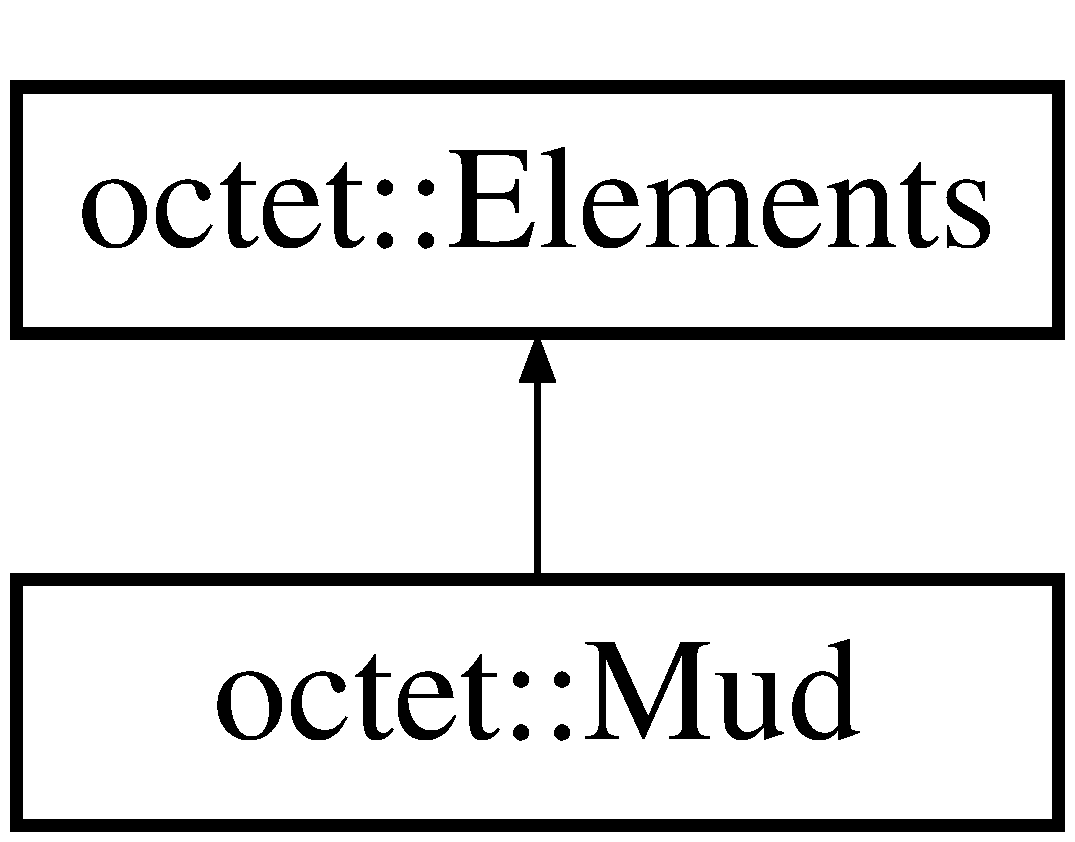
\includegraphics[height=2.000000cm]{structoctet_1_1_mud}
\end{center}
\end{figure}
\subsection*{Public Member Functions}
\begin{DoxyCompactItemize}
\item 
\hyperlink{structoctet_1_1_mud_af1a7da2f8b271943c445bb797b677076}{Mud} (int \hyperlink{structoctet_1_1_elements_a8d2c5872a3c685832f767505c85cf7e3}{index})
\end{DoxyCompactItemize}
\subsection*{Additional Inherited Members}


\subsection{Detailed Description}
The \hyperlink{structoctet_1_1_mud}{Mud} struct derived from the element struc. Only use to init the element This is use to init the element as a mud element. 

\subsection{Constructor \& Destructor Documentation}
\hypertarget{structoctet_1_1_mud_af1a7da2f8b271943c445bb797b677076}{\index{octet\+::\+Mud@{octet\+::\+Mud}!Mud@{Mud}}
\index{Mud@{Mud}!octet\+::\+Mud@{octet\+::\+Mud}}
\subsubsection[{Mud}]{\setlength{\rightskip}{0pt plus 5cm}octet\+::\+Mud\+::\+Mud (
\begin{DoxyParamCaption}
\item[{int}]{index}
\end{DoxyParamCaption}
)\hspace{0.3cm}{\ttfamily [inline]}}}\label{structoctet_1_1_mud_af1a7da2f8b271943c445bb797b677076}


The documentation for this struct was generated from the following file\+:\begin{DoxyCompactItemize}
\item 
\hyperlink{minecraft__wars_8h}{minecraft\+\_\+wars.\+h}\end{DoxyCompactItemize}

\hypertarget{structoctet_1_1_player}{\section{octet\+:\+:Player Struct Reference}
\label{structoctet_1_1_player}\index{octet\+::\+Player@{octet\+::\+Player}}
}


The \hyperlink{structoctet_1_1_player}{Player} struct contains all the relivent info about the player This is the object class for the player.  




{\ttfamily \#include $<$minecraft\+\_\+wars.\+h$>$}

\subsection*{Public Member Functions}
\begin{DoxyCompactItemize}
\item 
\hyperlink{structoctet_1_1_player_a8de855145bcf188d660ff1d9d4246753}{Player} ()
\begin{DoxyCompactList}\small\item\em The constructor for the player struct. \end{DoxyCompactList}\item 
bool \hyperlink{structoctet_1_1_player_a13aa8303245371b0fe4a27dedfb4c407}{Got\+\_\+\+Hit} (float damage)
\begin{DoxyCompactList}\small\item\em The ammont of damage the player has taken from the \hyperlink{structoctet_1_1_a_i}{A\+I} returns false if player dies. \end{DoxyCompactList}\item 
void \hyperlink{structoctet_1_1_player_a81bdc1d052b577d6f903863e1b75d985}{Element\+\_\+\+Picked} (int element\+\_\+number, int element\+\_\+index)
\begin{DoxyCompactList}\small\item\em used to manage the elemets\+\_\+held and the I\+D of those elements when the player picks up an element \end{DoxyCompactList}\item 
int \hyperlink{structoctet_1_1_player_ae4042f98a122ecf6cb43b43ef11452d7}{Element\+\_\+\+Placed} (int element\+\_\+number)
\begin{DoxyCompactList}\small\item\em used to manage the elemets\+\_\+held and the I\+D of those elements when the player places an element \end{DoxyCompactList}\item 
void \hyperlink{structoctet_1_1_player_ab1d777f5bee592f8cb1a733538fe1e5e}{Ammo\+\_\+\+Picked} (int weapon\+\_\+nu, int amount)
\begin{DoxyCompactList}\small\item\em used to manage the ammo when the player picks up ammo for a weapon \end{DoxyCompactList}\item 
bool \hyperlink{structoctet_1_1_player_a3c5f8a869d270b1a91830f2543f43901}{Weapon\+\_\+fired} (int weapon\+\_\+nu)
\begin{DoxyCompactList}\small\item\em used to manage the ammo when the player fires a weapon \end{DoxyCompactList}\end{DoxyCompactItemize}
\subsection*{Public Attributes}
\begin{DoxyCompactItemize}
\item 
float \hyperlink{structoctet_1_1_player_a2bdd50ed81043241cc239cd858e6fabb}{health}
\begin{DoxyCompactList}\small\item\em The current health of the player. \end{DoxyCompactList}\item 
int \hyperlink{structoctet_1_1_player_a52efa1d95f5bdf41f0fe427339b55801}{elements\+\_\+held} \mbox{[}\hyperlink{minecraft__wars_8h_a6e7de24a0c77478471e22ff642696cba}{Nu\+\_\+\+Elements}\mbox{]}
\begin{DoxyCompactList}\small\item\em The current elements held by the player. \end{DoxyCompactList}\item 
dynarray$<$ int $>$ \hyperlink{structoctet_1_1_player_a7d368ab73cce8c40a836e0b14a858c6c}{elements\+\_\+held\+\_\+ids} \mbox{[}\hyperlink{minecraft__wars_8h_a6e7de24a0c77478471e22ff642696cba}{Nu\+\_\+\+Elements}\mbox{]}
\begin{DoxyCompactList}\small\item\em The I\+Ds of the current elements held by the player. \end{DoxyCompactList}\item 
int \hyperlink{structoctet_1_1_player_a2076979db0f255de49747f1cfc0d2c56}{ammo} \mbox{[}\hyperlink{minecraft__wars_8h_acb18bb521c73ece6bfc2790c9bb0a83a}{Nu\+\_\+\+Weapon}\mbox{]}
\begin{DoxyCompactList}\small\item\em The ammon for the weapon held by the player. \end{DoxyCompactList}\item 
float \hyperlink{structoctet_1_1_player_aea38c028487f7b6049478fa68cc9a493}{weapon\+\_\+damage} \mbox{[}\hyperlink{minecraft__wars_8h_acb18bb521c73ece6bfc2790c9bb0a83a}{Nu\+\_\+\+Weapon}\mbox{]}
\begin{DoxyCompactList}\small\item\em The damage for the weapon held by the player. \end{DoxyCompactList}\item 
int \hyperlink{structoctet_1_1_player_a2ec6d4e522ec40035a3ab5a3389147fe}{current\+\_\+element}
\begin{DoxyCompactList}\small\item\em The current element that the player can place. \end{DoxyCompactList}\item 
int \hyperlink{structoctet_1_1_player_a20425ffb04a95dd2403edf613aa3959a}{current\+\_\+weapon}
\begin{DoxyCompactList}\small\item\em The current weapon that the player can use. \end{DoxyCompactList}\item 
int \hyperlink{structoctet_1_1_player_abcbda97162f67c67328c6578e9bafe29}{index}
\begin{DoxyCompactList}\small\item\em The index of the player in game object dynarray. \end{DoxyCompactList}\end{DoxyCompactItemize}


\subsection{Detailed Description}
The \hyperlink{structoctet_1_1_player}{Player} struct contains all the relivent info about the player This is the object class for the player. 

\subsection{Constructor \& Destructor Documentation}
\hypertarget{structoctet_1_1_player_a8de855145bcf188d660ff1d9d4246753}{\index{octet\+::\+Player@{octet\+::\+Player}!Player@{Player}}
\index{Player@{Player}!octet\+::\+Player@{octet\+::\+Player}}
\subsubsection[{Player}]{\setlength{\rightskip}{0pt plus 5cm}octet\+::\+Player\+::\+Player (
\begin{DoxyParamCaption}
{}
\end{DoxyParamCaption}
)\hspace{0.3cm}{\ttfamily [inline]}}}\label{structoctet_1_1_player_a8de855145bcf188d660ff1d9d4246753}


The constructor for the player struct. 



\subsection{Member Function Documentation}
\hypertarget{structoctet_1_1_player_ab1d777f5bee592f8cb1a733538fe1e5e}{\index{octet\+::\+Player@{octet\+::\+Player}!Ammo\+\_\+\+Picked@{Ammo\+\_\+\+Picked}}
\index{Ammo\+\_\+\+Picked@{Ammo\+\_\+\+Picked}!octet\+::\+Player@{octet\+::\+Player}}
\subsubsection[{Ammo\+\_\+\+Picked}]{\setlength{\rightskip}{0pt plus 5cm}void octet\+::\+Player\+::\+Ammo\+\_\+\+Picked (
\begin{DoxyParamCaption}
\item[{int}]{weapon\+\_\+nu, }
\item[{int}]{amount}
\end{DoxyParamCaption}
)\hspace{0.3cm}{\ttfamily [inline]}}}\label{structoctet_1_1_player_ab1d777f5bee592f8cb1a733538fe1e5e}


used to manage the ammo when the player picks up ammo for a weapon 


\begin{DoxyParams}{Parameters}
{\em int} & weapon\+\_\+nu The I\+D for the weapon that the player has picked the ammo for \\
\hline
{\em int} & amount the amount of ammo he has picked \\
\hline
\end{DoxyParams}
\hypertarget{structoctet_1_1_player_a81bdc1d052b577d6f903863e1b75d985}{\index{octet\+::\+Player@{octet\+::\+Player}!Element\+\_\+\+Picked@{Element\+\_\+\+Picked}}
\index{Element\+\_\+\+Picked@{Element\+\_\+\+Picked}!octet\+::\+Player@{octet\+::\+Player}}
\subsubsection[{Element\+\_\+\+Picked}]{\setlength{\rightskip}{0pt plus 5cm}void octet\+::\+Player\+::\+Element\+\_\+\+Picked (
\begin{DoxyParamCaption}
\item[{int}]{element\+\_\+number, }
\item[{int}]{element\+\_\+index}
\end{DoxyParamCaption}
)\hspace{0.3cm}{\ttfamily [inline]}}}\label{structoctet_1_1_player_a81bdc1d052b577d6f903863e1b75d985}


used to manage the elemets\+\_\+held and the I\+D of those elements when the player picks up an element 


\begin{DoxyParams}{Parameters}
{\em int} & element\+\_\+number The I\+D of the element the player picked \\
\hline
{\em int} & element\+\_\+index The Index of that element in the game object dynarray \\
\hline
\end{DoxyParams}
\hypertarget{structoctet_1_1_player_ae4042f98a122ecf6cb43b43ef11452d7}{\index{octet\+::\+Player@{octet\+::\+Player}!Element\+\_\+\+Placed@{Element\+\_\+\+Placed}}
\index{Element\+\_\+\+Placed@{Element\+\_\+\+Placed}!octet\+::\+Player@{octet\+::\+Player}}
\subsubsection[{Element\+\_\+\+Placed}]{\setlength{\rightskip}{0pt plus 5cm}int octet\+::\+Player\+::\+Element\+\_\+\+Placed (
\begin{DoxyParamCaption}
\item[{int}]{element\+\_\+number}
\end{DoxyParamCaption}
)\hspace{0.3cm}{\ttfamily [inline]}}}\label{structoctet_1_1_player_ae4042f98a122ecf6cb43b43ef11452d7}


used to manage the elemets\+\_\+held and the I\+D of those elements when the player places an element 


\begin{DoxyParams}{Parameters}
{\em int} & element\+\_\+number The I\+D of the element the player picked \\
\hline
\end{DoxyParams}
\begin{DoxyReturn}{Returns}
an int the index of the element in the dynarray 
\end{DoxyReturn}
\hypertarget{structoctet_1_1_player_a13aa8303245371b0fe4a27dedfb4c407}{\index{octet\+::\+Player@{octet\+::\+Player}!Got\+\_\+\+Hit@{Got\+\_\+\+Hit}}
\index{Got\+\_\+\+Hit@{Got\+\_\+\+Hit}!octet\+::\+Player@{octet\+::\+Player}}
\subsubsection[{Got\+\_\+\+Hit}]{\setlength{\rightskip}{0pt plus 5cm}bool octet\+::\+Player\+::\+Got\+\_\+\+Hit (
\begin{DoxyParamCaption}
\item[{float}]{damage}
\end{DoxyParamCaption}
)\hspace{0.3cm}{\ttfamily [inline]}}}\label{structoctet_1_1_player_a13aa8303245371b0fe4a27dedfb4c407}


The ammont of damage the player has taken from the \hyperlink{structoctet_1_1_a_i}{A\+I} returns false if player dies. 

\begin{DoxyReturn}{Returns}
a bool true if player is alive false if dead 
\end{DoxyReturn}
\hypertarget{structoctet_1_1_player_a3c5f8a869d270b1a91830f2543f43901}{\index{octet\+::\+Player@{octet\+::\+Player}!Weapon\+\_\+fired@{Weapon\+\_\+fired}}
\index{Weapon\+\_\+fired@{Weapon\+\_\+fired}!octet\+::\+Player@{octet\+::\+Player}}
\subsubsection[{Weapon\+\_\+fired}]{\setlength{\rightskip}{0pt plus 5cm}bool octet\+::\+Player\+::\+Weapon\+\_\+fired (
\begin{DoxyParamCaption}
\item[{int}]{weapon\+\_\+nu}
\end{DoxyParamCaption}
)\hspace{0.3cm}{\ttfamily [inline]}}}\label{structoctet_1_1_player_a3c5f8a869d270b1a91830f2543f43901}


used to manage the ammo when the player fires a weapon 


\begin{DoxyParams}{Parameters}
{\em int} & weapon\+\_\+nu The I\+D for the weapon that the player has picked the ammo for \\
\hline
\end{DoxyParams}
\begin{DoxyReturn}{Returns}
a bool true if the player has ammo to fire that weapon false if he is out of ammo 
\end{DoxyReturn}


\subsection{Member Data Documentation}
\hypertarget{structoctet_1_1_player_a2076979db0f255de49747f1cfc0d2c56}{\index{octet\+::\+Player@{octet\+::\+Player}!ammo@{ammo}}
\index{ammo@{ammo}!octet\+::\+Player@{octet\+::\+Player}}
\subsubsection[{ammo}]{\setlength{\rightskip}{0pt plus 5cm}octet\+::\+Player\+::ammo\mbox{[}{\bf Nu\+\_\+\+Weapon}\mbox{]}}}\label{structoctet_1_1_player_a2076979db0f255de49747f1cfc0d2c56}


The ammon for the weapon held by the player. 

\hypertarget{structoctet_1_1_player_a2ec6d4e522ec40035a3ab5a3389147fe}{\index{octet\+::\+Player@{octet\+::\+Player}!current\+\_\+element@{current\+\_\+element}}
\index{current\+\_\+element@{current\+\_\+element}!octet\+::\+Player@{octet\+::\+Player}}
\subsubsection[{current\+\_\+element}]{\setlength{\rightskip}{0pt plus 5cm}int octet\+::\+Player\+::current\+\_\+element}}\label{structoctet_1_1_player_a2ec6d4e522ec40035a3ab5a3389147fe}


The current element that the player can place. 

\hypertarget{structoctet_1_1_player_a20425ffb04a95dd2403edf613aa3959a}{\index{octet\+::\+Player@{octet\+::\+Player}!current\+\_\+weapon@{current\+\_\+weapon}}
\index{current\+\_\+weapon@{current\+\_\+weapon}!octet\+::\+Player@{octet\+::\+Player}}
\subsubsection[{current\+\_\+weapon}]{\setlength{\rightskip}{0pt plus 5cm}int octet\+::\+Player\+::current\+\_\+weapon}}\label{structoctet_1_1_player_a20425ffb04a95dd2403edf613aa3959a}


The current weapon that the player can use. 

\hypertarget{structoctet_1_1_player_a52efa1d95f5bdf41f0fe427339b55801}{\index{octet\+::\+Player@{octet\+::\+Player}!elements\+\_\+held@{elements\+\_\+held}}
\index{elements\+\_\+held@{elements\+\_\+held}!octet\+::\+Player@{octet\+::\+Player}}
\subsubsection[{elements\+\_\+held}]{\setlength{\rightskip}{0pt plus 5cm}int octet\+::\+Player\+::elements\+\_\+held\mbox{[}{\bf Nu\+\_\+\+Elements}\mbox{]}}}\label{structoctet_1_1_player_a52efa1d95f5bdf41f0fe427339b55801}


The current elements held by the player. 

\hypertarget{structoctet_1_1_player_a7d368ab73cce8c40a836e0b14a858c6c}{\index{octet\+::\+Player@{octet\+::\+Player}!elements\+\_\+held\+\_\+ids@{elements\+\_\+held\+\_\+ids}}
\index{elements\+\_\+held\+\_\+ids@{elements\+\_\+held\+\_\+ids}!octet\+::\+Player@{octet\+::\+Player}}
\subsubsection[{elements\+\_\+held\+\_\+ids}]{\setlength{\rightskip}{0pt plus 5cm}dynarray$<$ int $>$ octet\+::\+Player\+::elements\+\_\+held\+\_\+ids\mbox{[}{\bf Nu\+\_\+\+Elements}\mbox{]}}}\label{structoctet_1_1_player_a7d368ab73cce8c40a836e0b14a858c6c}


The I\+Ds of the current elements held by the player. 

\hypertarget{structoctet_1_1_player_a2bdd50ed81043241cc239cd858e6fabb}{\index{octet\+::\+Player@{octet\+::\+Player}!health@{health}}
\index{health@{health}!octet\+::\+Player@{octet\+::\+Player}}
\subsubsection[{health}]{\setlength{\rightskip}{0pt plus 5cm}float octet\+::\+Player\+::health}}\label{structoctet_1_1_player_a2bdd50ed81043241cc239cd858e6fabb}


The current health of the player. 

\hypertarget{structoctet_1_1_player_abcbda97162f67c67328c6578e9bafe29}{\index{octet\+::\+Player@{octet\+::\+Player}!index@{index}}
\index{index@{index}!octet\+::\+Player@{octet\+::\+Player}}
\subsubsection[{index}]{\setlength{\rightskip}{0pt plus 5cm}int octet\+::\+Player\+::index}}\label{structoctet_1_1_player_abcbda97162f67c67328c6578e9bafe29}


The index of the player in game object dynarray. 

\hypertarget{structoctet_1_1_player_aea38c028487f7b6049478fa68cc9a493}{\index{octet\+::\+Player@{octet\+::\+Player}!weapon\+\_\+damage@{weapon\+\_\+damage}}
\index{weapon\+\_\+damage@{weapon\+\_\+damage}!octet\+::\+Player@{octet\+::\+Player}}
\subsubsection[{weapon\+\_\+damage}]{\setlength{\rightskip}{0pt plus 5cm}float octet\+::\+Player\+::weapon\+\_\+damage\mbox{[}{\bf Nu\+\_\+\+Weapon}\mbox{]}}}\label{structoctet_1_1_player_aea38c028487f7b6049478fa68cc9a493}


The damage for the weapon held by the player. 



The documentation for this struct was generated from the following file\+:\begin{DoxyCompactItemize}
\item 
\hyperlink{minecraft__wars_8h}{minecraft\+\_\+wars.\+h}\end{DoxyCompactItemize}

\hypertarget{structoctet_1_1_stone}{\section{octet\+:\+:Stone Struct Reference}
\label{structoctet_1_1_stone}\index{octet\+::\+Stone@{octet\+::\+Stone}}
}


The \hyperlink{structoctet_1_1_stone}{Stone} struct derived from the element struc. Only use to init the element This is use to init the element as a stone element.  




{\ttfamily \#include $<$minecraft\+\_\+wars.\+h$>$}

Inheritance diagram for octet\+:\+:Stone\+:\begin{figure}[H]
\begin{center}
\leavevmode
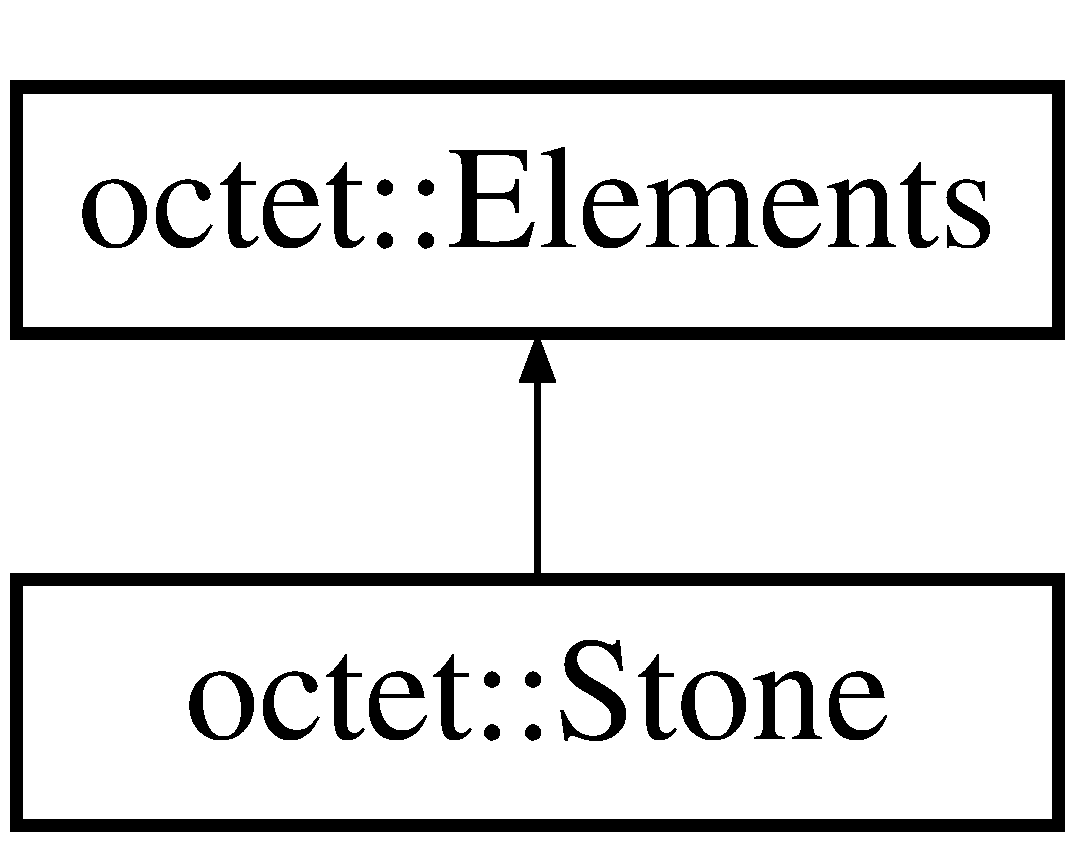
\includegraphics[height=2.000000cm]{structoctet_1_1_stone}
\end{center}
\end{figure}
\subsection*{Public Member Functions}
\begin{DoxyCompactItemize}
\item 
\hyperlink{structoctet_1_1_stone_a434992c11c68d58b8e5758b584d98771}{Stone} (int \hyperlink{structoctet_1_1_elements_a8d2c5872a3c685832f767505c85cf7e3}{index})
\end{DoxyCompactItemize}
\subsection*{Additional Inherited Members}


\subsection{Detailed Description}
The \hyperlink{structoctet_1_1_stone}{Stone} struct derived from the element struc. Only use to init the element This is use to init the element as a stone element. 

The \hyperlink{structoctet_1_1_iron}{Iron} struct derived from the element struc. Only use to init the element This is use to init the element as an iron element. 

\subsection{Constructor \& Destructor Documentation}
\hypertarget{structoctet_1_1_stone_a434992c11c68d58b8e5758b584d98771}{\index{octet\+::\+Stone@{octet\+::\+Stone}!Stone@{Stone}}
\index{Stone@{Stone}!octet\+::\+Stone@{octet\+::\+Stone}}
\subsubsection[{Stone}]{\setlength{\rightskip}{0pt plus 5cm}octet\+::\+Stone\+::\+Stone (
\begin{DoxyParamCaption}
\item[{int}]{index}
\end{DoxyParamCaption}
)\hspace{0.3cm}{\ttfamily [inline]}}}\label{structoctet_1_1_stone_a434992c11c68d58b8e5758b584d98771}


The documentation for this struct was generated from the following file\+:\begin{DoxyCompactItemize}
\item 
\hyperlink{minecraft__wars_8h}{minecraft\+\_\+wars.\+h}\end{DoxyCompactItemize}

\hypertarget{structoctet_1_1_wood}{\section{octet\+:\+:Wood Struct Reference}
\label{structoctet_1_1_wood}\index{octet\+::\+Wood@{octet\+::\+Wood}}
}


The \hyperlink{structoctet_1_1_wood}{Wood} struct derived from the element struc. Only use to init the element This is use to init the element as a wood element.  




{\ttfamily \#include $<$minecraft\+\_\+wars.\+h$>$}

Inheritance diagram for octet\+:\+:Wood\+:\begin{figure}[H]
\begin{center}
\leavevmode
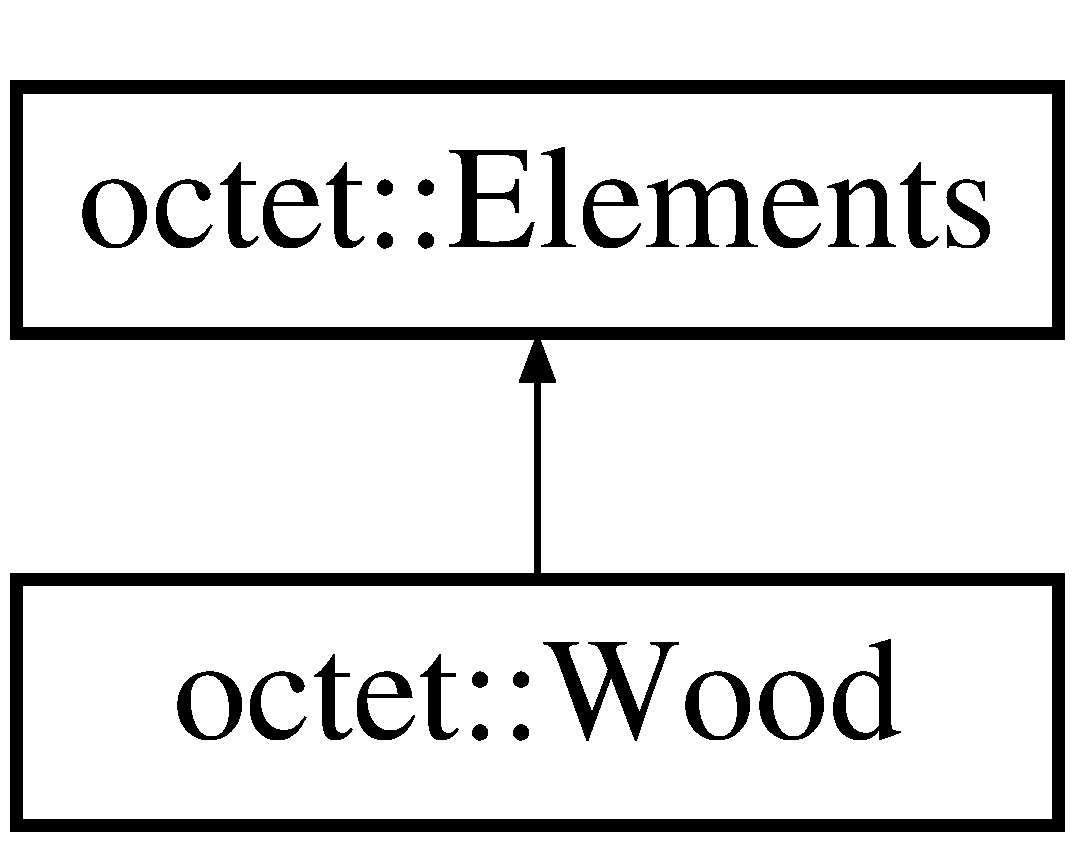
\includegraphics[height=2.000000cm]{structoctet_1_1_wood}
\end{center}
\end{figure}
\subsection*{Public Member Functions}
\begin{DoxyCompactItemize}
\item 
\hyperlink{structoctet_1_1_wood_a227c533366647f139c29085e8bc511dc}{Wood} (int \hyperlink{structoctet_1_1_elements_a8d2c5872a3c685832f767505c85cf7e3}{index})
\end{DoxyCompactItemize}
\subsection*{Additional Inherited Members}


\subsection{Detailed Description}
The \hyperlink{structoctet_1_1_wood}{Wood} struct derived from the element struc. Only use to init the element This is use to init the element as a wood element. 

\subsection{Constructor \& Destructor Documentation}
\hypertarget{structoctet_1_1_wood_a227c533366647f139c29085e8bc511dc}{\index{octet\+::\+Wood@{octet\+::\+Wood}!Wood@{Wood}}
\index{Wood@{Wood}!octet\+::\+Wood@{octet\+::\+Wood}}
\subsubsection[{Wood}]{\setlength{\rightskip}{0pt plus 5cm}octet\+::\+Wood\+::\+Wood (
\begin{DoxyParamCaption}
\item[{int}]{index}
\end{DoxyParamCaption}
)\hspace{0.3cm}{\ttfamily [inline]}}}\label{structoctet_1_1_wood_a227c533366647f139c29085e8bc511dc}


The documentation for this struct was generated from the following file\+:\begin{DoxyCompactItemize}
\item 
\hyperlink{minecraft__wars_8h}{minecraft\+\_\+wars.\+h}\end{DoxyCompactItemize}

\chapter{File Documentation}
\hypertarget{main_8cpp}{\section{main.\+cpp File Reference}
\label{main_8cpp}\index{main.\+cpp@{main.\+cpp}}
}
{\ttfamily \#include \char`\"{}../../octet.\+h\char`\"{}}\\*
{\ttfamily \#include \char`\"{}minecraft\+\_\+wars.\+h\char`\"{}}\\*
\subsection*{Macros}
\begin{DoxyCompactItemize}
\item 
\#define \hyperlink{main_8cpp_a34ab1cc8340de6c0d94ed7d0fa877c98}{O\+C\+T\+E\+T\+\_\+\+B\+U\+L\+L\+E\+T}~1
\end{DoxyCompactItemize}
\subsection*{Functions}
\begin{DoxyCompactItemize}
\item 
int \hyperlink{main_8cpp_a3c04138a5bfe5d72780bb7e82a18e627}{main} (int argc, char $\ast$$\ast$argv)
\begin{DoxyCompactList}\small\item\em Create a box with octet. \end{DoxyCompactList}\end{DoxyCompactItemize}


\subsection{Macro Definition Documentation}
\hypertarget{main_8cpp_a34ab1cc8340de6c0d94ed7d0fa877c98}{\index{main.\+cpp@{main.\+cpp}!O\+C\+T\+E\+T\+\_\+\+B\+U\+L\+L\+E\+T@{O\+C\+T\+E\+T\+\_\+\+B\+U\+L\+L\+E\+T}}
\index{O\+C\+T\+E\+T\+\_\+\+B\+U\+L\+L\+E\+T@{O\+C\+T\+E\+T\+\_\+\+B\+U\+L\+L\+E\+T}!main.\+cpp@{main.\+cpp}}
\subsubsection[{O\+C\+T\+E\+T\+\_\+\+B\+U\+L\+L\+E\+T}]{\setlength{\rightskip}{0pt plus 5cm}\#define O\+C\+T\+E\+T\+\_\+\+B\+U\+L\+L\+E\+T~1}}\label{main_8cpp_a34ab1cc8340de6c0d94ed7d0fa877c98}


\subsection{Function Documentation}
\hypertarget{main_8cpp_a3c04138a5bfe5d72780bb7e82a18e627}{\index{main.\+cpp@{main.\+cpp}!main@{main}}
\index{main@{main}!main.\+cpp@{main.\+cpp}}
\subsubsection[{main}]{\setlength{\rightskip}{0pt plus 5cm}int main (
\begin{DoxyParamCaption}
\item[{int}]{argc, }
\item[{char $\ast$$\ast$}]{argv}
\end{DoxyParamCaption}
)}}\label{main_8cpp_a3c04138a5bfe5d72780bb7e82a18e627}


Create a box with octet. 


\hypertarget{minecraft__wars_8h}{\section{minecraft\+\_\+wars.\+h File Reference}
\label{minecraft__wars_8h}\index{minecraft\+\_\+wars.\+h@{minecraft\+\_\+wars.\+h}}
}
\subsection*{Classes}
\begin{DoxyCompactItemize}
\item 
class \hyperlink{classoctet_1_1_collision_objects}{octet\+::\+Collision\+Objects}
\begin{DoxyCompactList}\small\item\em this class stores the basic common information about the game objects ie I\+D, Rigidbody, and the pointer to the specific object. all game object that are rigid bodies are objects of this class. \end{DoxyCompactList}\item 
struct \hyperlink{structoctet_1_1_player}{octet\+::\+Player}
\begin{DoxyCompactList}\small\item\em The \hyperlink{structoctet_1_1_player}{Player} struct contains all the relivent info about the player This is the object class for the player. \end{DoxyCompactList}\item 
struct \hyperlink{structoctet_1_1_a_i}{octet\+::\+A\+I}
\begin{DoxyCompactList}\small\item\em The \hyperlink{structoctet_1_1_a_i}{A\+I} struct contains all the relivent info about the \hyperlink{structoctet_1_1_a_i}{A\+I} This is the object class for the \hyperlink{structoctet_1_1_a_i}{A\+I}. \end{DoxyCompactList}\item 
struct \hyperlink{structoctet_1_1_elements}{octet\+::\+Elements}
\begin{DoxyCompactList}\small\item\em The base struct for all the elements.\+Use this in the userpointer and call the derived class constructors to init this This is the object class for all the elements. \end{DoxyCompactList}\item 
struct \hyperlink{structoctet_1_1_mud}{octet\+::\+Mud}
\begin{DoxyCompactList}\small\item\em The \hyperlink{structoctet_1_1_mud}{Mud} struct derived from the element struc. Only use to init the element This is use to init the element as a mud element. \end{DoxyCompactList}\item 
struct \hyperlink{structoctet_1_1_wood}{octet\+::\+Wood}
\begin{DoxyCompactList}\small\item\em The \hyperlink{structoctet_1_1_wood}{Wood} struct derived from the element struc. Only use to init the element This is use to init the element as a wood element. \end{DoxyCompactList}\item 
struct \hyperlink{structoctet_1_1_stone}{octet\+::\+Stone}
\begin{DoxyCompactList}\small\item\em The \hyperlink{structoctet_1_1_stone}{Stone} struct derived from the element struc. Only use to init the element This is use to init the element as a stone element. \end{DoxyCompactList}\item 
struct \hyperlink{structoctet_1_1_iron}{octet\+::\+Iron}
\item 
class \hyperlink{classoctet_1_1minecraft__wars}{octet\+::minecraft\+\_\+wars}
\begin{DoxyCompactList}\small\item\em this is the main class of this project. \end{DoxyCompactList}\end{DoxyCompactItemize}
\subsection*{Namespaces}
\begin{DoxyCompactItemize}
\item 
 \hyperlink{namespaceoctet}{octet}
\begin{DoxyCompactList}\small\item\em Minecraft Wars 2014 \+: A simple project in which the player has to collect elements, build a fort, and defend his fort as long as he can. \end{DoxyCompactList}\end{DoxyCompactItemize}
\subsection*{Macros}
\begin{DoxyCompactItemize}
\item 
\#define \hyperlink{minecraft__wars_8h_a6e7de24a0c77478471e22ff642696cba}{Nu\+\_\+\+Elements}~4
\begin{DoxyCompactList}\small\item\em The Number of elements in the game ie \+: Mud, Wood, Stone, Iron. \end{DoxyCompactList}\item 
\#define \hyperlink{minecraft__wars_8h_acb18bb521c73ece6bfc2790c9bb0a83a}{Nu\+\_\+\+Weapon}~1
\begin{DoxyCompactList}\small\item\em The Number of weapons in the game ie \+: gun. \end{DoxyCompactList}\end{DoxyCompactItemize}
\subsection*{Enumerations}
\begin{DoxyCompactItemize}
\item 
enum \hyperlink{namespaceoctet_ae14a40f56acaed04355429b24bf458e7}{octet\+::\+I\+D\+\_\+\+Object} \{ \\*
\hyperlink{namespaceoctet_ae14a40f56acaed04355429b24bf458e7a491b9ccf81c178214d49a98b2d33b042}{octet\+::\+Plane\+\_\+\+I\+D} = -\/1, 
\hyperlink{namespaceoctet_ae14a40f56acaed04355429b24bf458e7a5c20c8692e98f9f94883e6bcc8fd12dc}{octet\+::\+Player\+\_\+\+I\+D} = 0, 
\hyperlink{namespaceoctet_ae14a40f56acaed04355429b24bf458e7ab803c5aaf40caa6eaff50efa4aad3506}{octet\+::\+Element\+\_\+\+I\+D} = 1, 
\hyperlink{namespaceoctet_ae14a40f56acaed04355429b24bf458e7a3d19bfd0716876c3d201134677de2d94}{octet\+::\+A\+I\+\_\+\+I\+D} = 2, 
\\*
\hyperlink{namespaceoctet_ae14a40f56acaed04355429b24bf458e7a58b4b5a7969f17157696f9691a807c16}{octet\+::\+Pickup\+\_\+\+I\+D} = 3
 \}
\begin{DoxyCompactList}\small\item\em This enum contains the I\+Ds for the game objects. Used to check what kind of an object the rigid body is from the user pointer. \end{DoxyCompactList}\item 
enum \hyperlink{namespaceoctet_a25293ed69f50158637344e438fa1ae72}{octet\+::\+I\+D\+\_\+\+Pickup} \{ \hyperlink{namespaceoctet_a25293ed69f50158637344e438fa1ae72a3d0d227c0fe13d73d160e1b8b1ddb531}{octet\+::\+Health\+\_\+\+I\+D} = 0, 
\hyperlink{namespaceoctet_a25293ed69f50158637344e438fa1ae72a0c567823ad645972eb32082eb093f016}{octet\+::\+Ammo\+\_\+\+I\+D} = 1
 \}
\begin{DoxyCompactList}\small\item\em This enum contains the I\+Ds for the items the player can pick. \end{DoxyCompactList}\item 
enum \hyperlink{namespaceoctet_a8a658c1664b86192b093101b410d8e22}{octet\+::\+I\+D\+\_\+\+Element} \{ \hyperlink{namespaceoctet_a8a658c1664b86192b093101b410d8e22a324ef69f1bb1cbe448bac355a6454f8d}{octet\+::\+Mud\+\_\+\+I\+D} = 0, 
\hyperlink{namespaceoctet_a8a658c1664b86192b093101b410d8e22a9df8ab8e26428d27934e8f4006ec4ff0}{octet\+::\+Wood\+\_\+\+I\+D} = 1, 
\hyperlink{namespaceoctet_a8a658c1664b86192b093101b410d8e22a7c55c376037f3e0568e5afdd52712e2f}{octet\+::\+Stone\+\_\+\+I\+D} = 2, 
\hyperlink{namespaceoctet_a8a658c1664b86192b093101b410d8e22a4199137749094f74e555cde8146bbedf}{octet\+::\+Iron\+\_\+\+I\+D} = 3
 \}
\begin{DoxyCompactList}\small\item\em This enum contains the I\+Ds for the elements the game will have. \end{DoxyCompactList}\item 
enum \hyperlink{namespaceoctet_a9b5c767b2f5906d32938347f219f29d8}{octet\+::\+I\+D\+\_\+weapon} \{ \hyperlink{namespaceoctet_a9b5c767b2f5906d32938347f219f29d8aba4bbd933933361c95782aeef88f84b6}{octet\+::\+Gun\+\_\+\+I\+D} = 0
 \}
\begin{DoxyCompactList}\small\item\em This enum contains the I\+Ds for the weapons the game will have. \end{DoxyCompactList}\item 
enum \hyperlink{namespaceoctet_ae8a703c3351a9f48aa7ad96fc57c55b4}{octet\+::\+Hits\+\_\+to\+\_\+extract\+\_\+\+Element} \{ \hyperlink{namespaceoctet_ae8a703c3351a9f48aa7ad96fc57c55b4a750c23f53924dfbcd9fb50ca61e8f480}{octet\+::\+Mud\+\_\+\+Hits} = 2, 
\hyperlink{namespaceoctet_ae8a703c3351a9f48aa7ad96fc57c55b4a7827d8f1739c787a24f280dd43555860}{octet\+::\+Wood\+\_\+\+Hits} = 3, 
\hyperlink{namespaceoctet_ae8a703c3351a9f48aa7ad96fc57c55b4aed66fa47b7558f768b7e5e30cd526e89}{octet\+::\+Stone\+\_\+\+Hits} = 5, 
\hyperlink{namespaceoctet_ae8a703c3351a9f48aa7ad96fc57c55b4a05e2baa4de05be589af50ab12a54ab67}{octet\+::\+Iron\+\_\+\+Hits} = 7
 \}
\begin{DoxyCompactList}\small\item\em This enum contains the number of gather hits required by the player to gather a perticular element. \end{DoxyCompactList}\end{DoxyCompactItemize}
\subsection*{Functions}
\begin{DoxyCompactItemize}
\item 
bool \hyperlink{namespaceoctet_a18649e9a2945ba720f8b1454433bffb9}{octet\+::\+A\+Iisfacingobject} (bt\+Rigid\+Body $\ast$A\+I, bt\+Rigid\+Body $\ast$obj)
\begin{DoxyCompactList}\small\item\em This fucntion is called when the \hyperlink{structoctet_1_1_a_i}{A\+I} collides with an element or the player to check if the \hyperlink{structoctet_1_1_a_i}{A\+I} is facing then to attack. \end{DoxyCompactList}\item 
bool \hyperlink{namespaceoctet_a612adfaf8e4ba9b7d22fec5b9a2672b7}{octet\+::minecraftcollision} (bt\+Manifold\+Point \&cp, const bt\+Collision\+Object\+Wrapper $\ast$obj1, int id1, int index1, const bt\+Collision\+Object\+Wrapper $\ast$obj2, int id2, int index2)
\begin{DoxyCompactList}\small\item\em The collision custom callback fucntion.\+This is called when a collion takes place. \end{DoxyCompactList}\end{DoxyCompactItemize}


\subsection{Macro Definition Documentation}
\hypertarget{minecraft__wars_8h_a6e7de24a0c77478471e22ff642696cba}{\index{minecraft\+\_\+wars.\+h@{minecraft\+\_\+wars.\+h}!Nu\+\_\+\+Elements@{Nu\+\_\+\+Elements}}
\index{Nu\+\_\+\+Elements@{Nu\+\_\+\+Elements}!minecraft\+\_\+wars.\+h@{minecraft\+\_\+wars.\+h}}
\subsubsection[{Nu\+\_\+\+Elements}]{\setlength{\rightskip}{0pt plus 5cm}\#define Nu\+\_\+\+Elements~4}}\label{minecraft__wars_8h_a6e7de24a0c77478471e22ff642696cba}


The Number of elements in the game ie \+: Mud, Wood, Stone, Iron. 

\hypertarget{minecraft__wars_8h_acb18bb521c73ece6bfc2790c9bb0a83a}{\index{minecraft\+\_\+wars.\+h@{minecraft\+\_\+wars.\+h}!Nu\+\_\+\+Weapon@{Nu\+\_\+\+Weapon}}
\index{Nu\+\_\+\+Weapon@{Nu\+\_\+\+Weapon}!minecraft\+\_\+wars.\+h@{minecraft\+\_\+wars.\+h}}
\subsubsection[{Nu\+\_\+\+Weapon}]{\setlength{\rightskip}{0pt plus 5cm}\#define Nu\+\_\+\+Weapon~1}}\label{minecraft__wars_8h_acb18bb521c73ece6bfc2790c9bb0a83a}


The Number of weapons in the game ie \+: gun. 


\hypertarget{_r_e_a_d_m_e_8md}{\section{R\+E\+A\+D\+M\+E.\+md File Reference}
\label{_r_e_a_d_m_e_8md}\index{R\+E\+A\+D\+M\+E.\+md@{R\+E\+A\+D\+M\+E.\+md}}
}

%--- End generated contents ---

% Index
\newpage
\phantomsection
\addcontentsline{toc}{chapter}{Index}
\printindex

\end{document}
